% REMOVE \caption{} to remove in LIST OF FIGURES

\begin{doublespace}
	\begin{center}
		\app{Survey and Assessment Form}
% \subsection*{APPENDIX A} \label{appendixa}
\null\vfill\appendixform{1}{1}\vfill
\null\vfill\appendixform{1}{2}\vfill
\null\vfill\appendixform{1}{3}\vfill
\null\vfill\appendixform{1}{5}\vfill
\null\vfill\appendixform{1}{5}\vfill
\null\vfill\appendixform{1}{6}\vfill
\null\vfill\appendixform{1}{7}\vfill
\null\vfill\appendixform{1}{8}\vfill
\null\vfill\appendixform{1}{9}\vfill
\null\vfill\appendixform{1}{11}\vfill
% \appfig{Assessment Form}
\null\vfill\appendixform{2}{1}\vfill
\null\vfill\appendixform{2}{2}\vfill
\null\vfill\appendixform{2}{3}\vfill
\null\vfill\appendixform{2}{4}\vfill
\null\vfill\appendixform{2}{5}\vfill
% \appfig{Survey Form}

		\clearpage
\app{Evaluation Form}
\null\vfill
\begin{figure}[H]
	 \centering
	 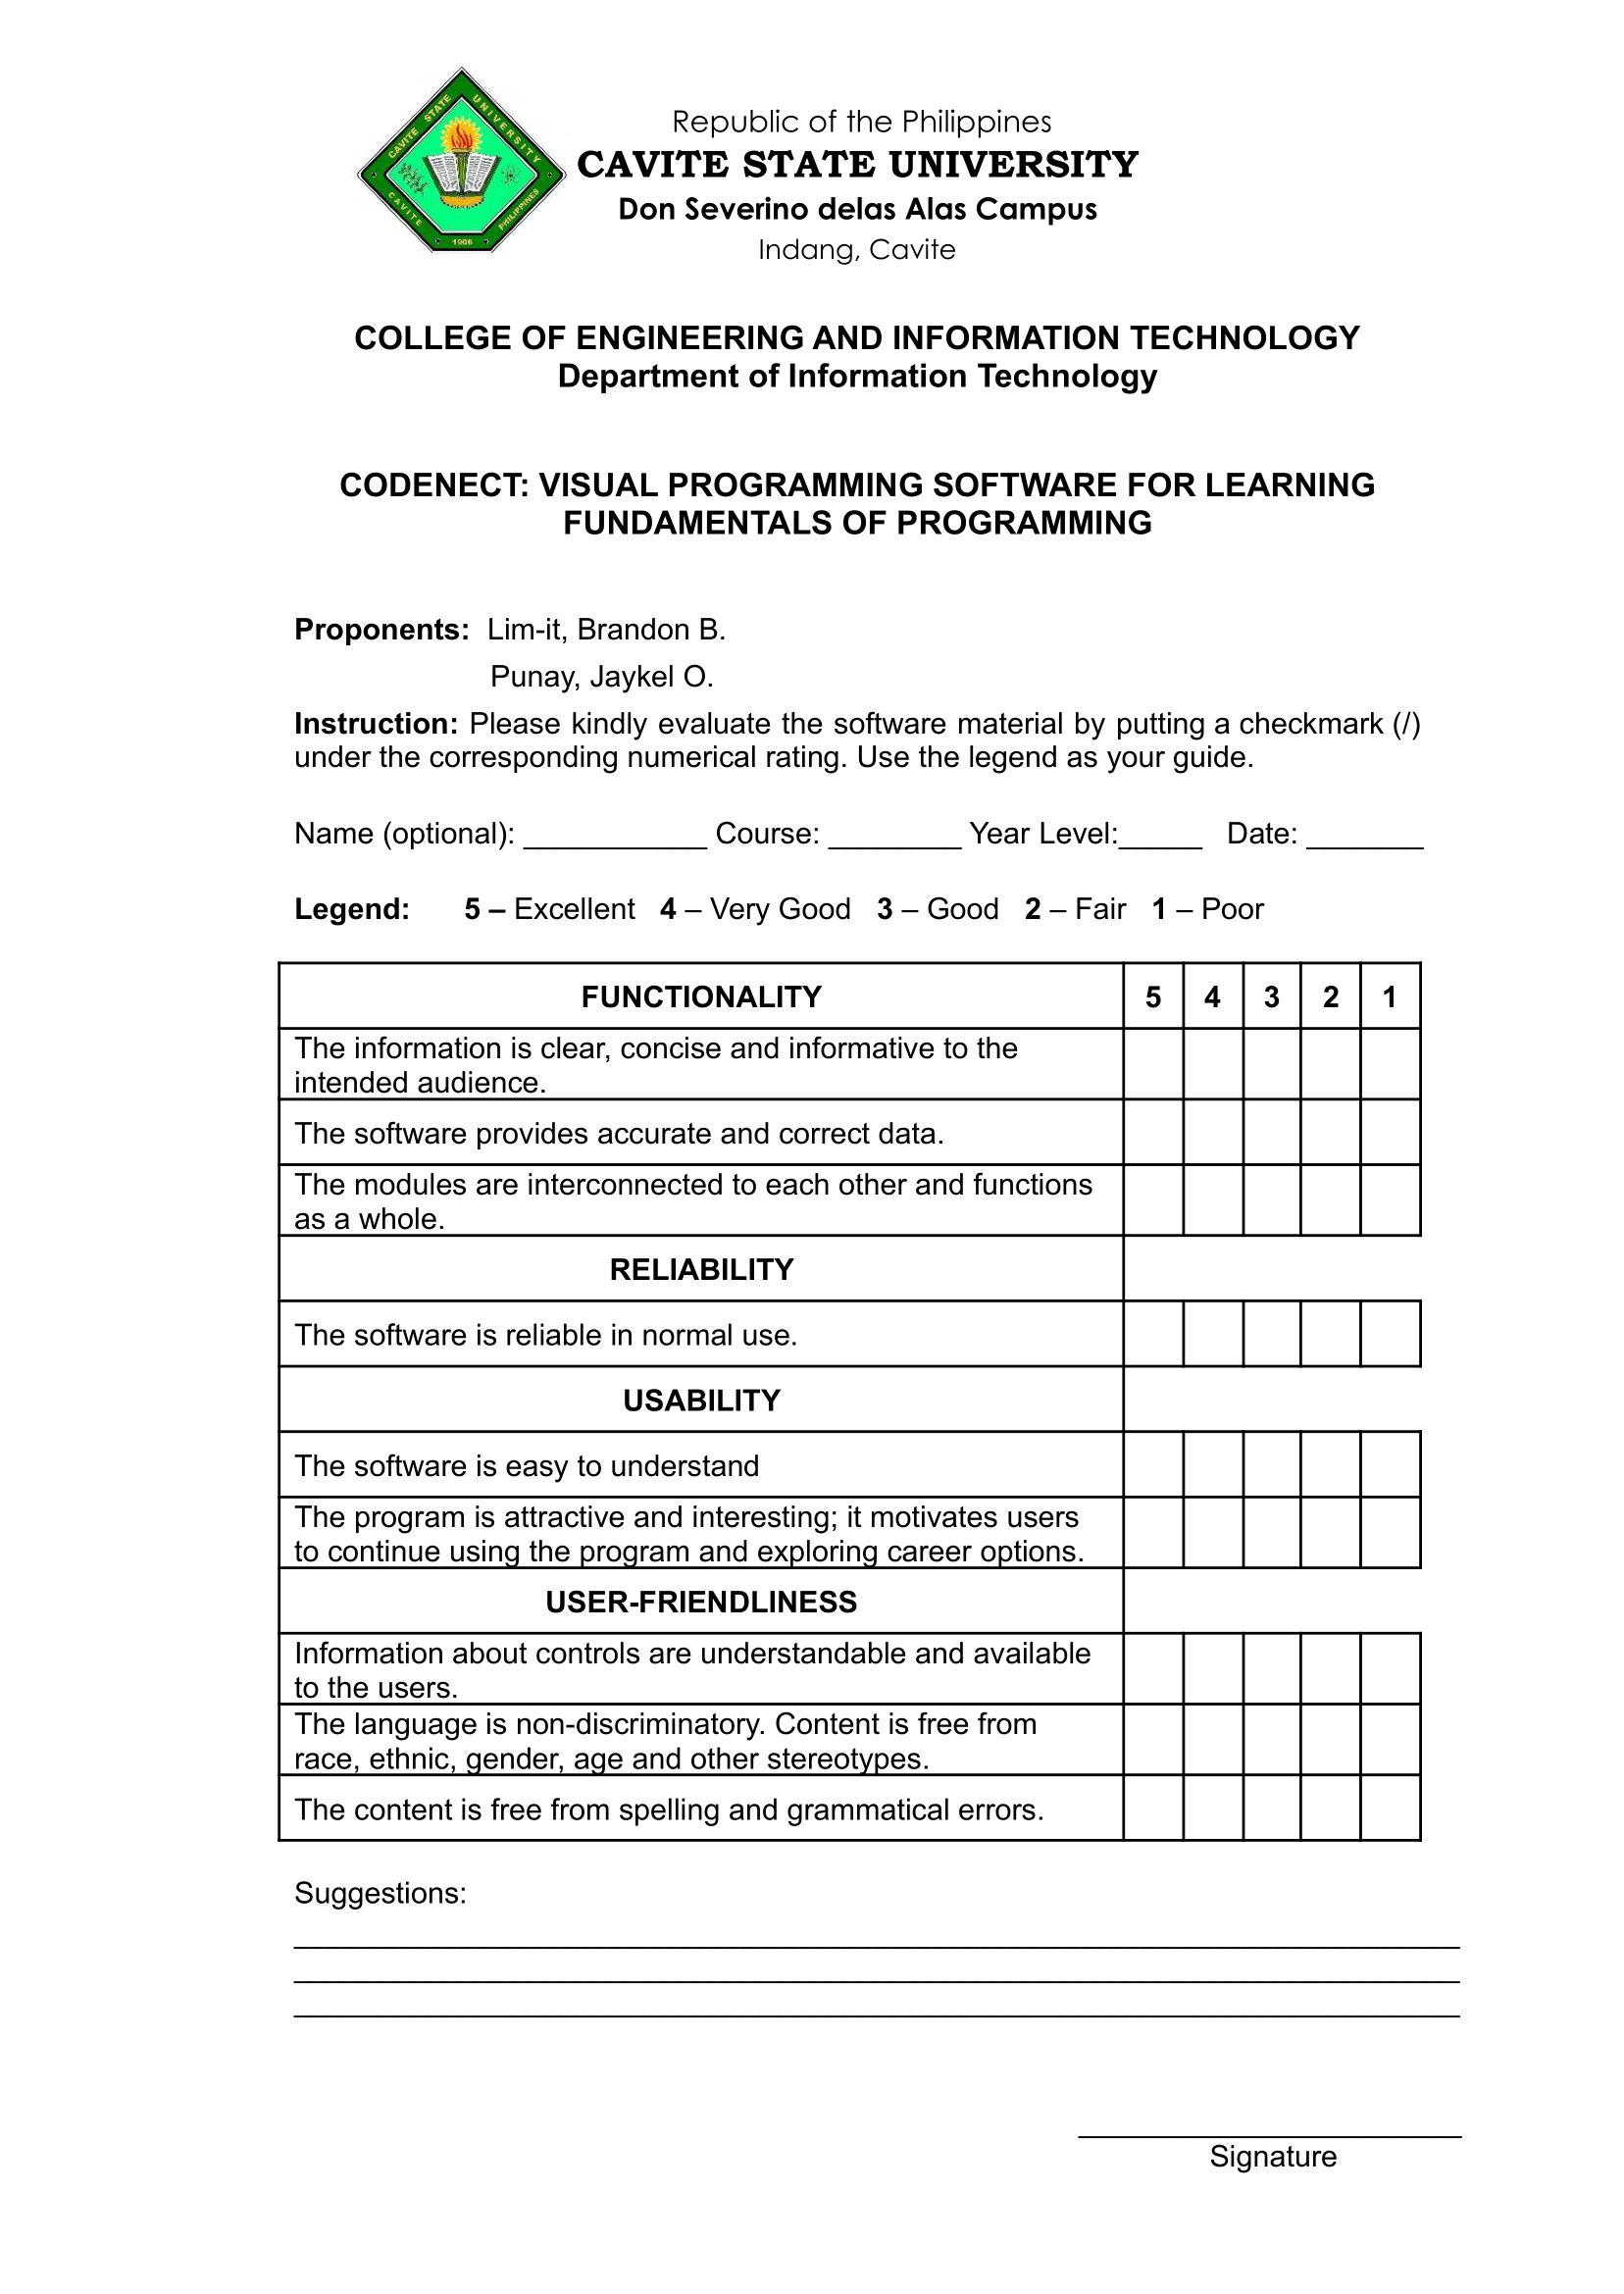
\includegraphics[width=\textwidth]{figures/non_tech_eval_form.png}
	 \caption[]{Non-Technical Evaluation Form}
	 \label{fig:non_tech_eval_form}
\end{figure}

\clearpage
\null\vfill
\begin{figure}[H]
	 \centering
	 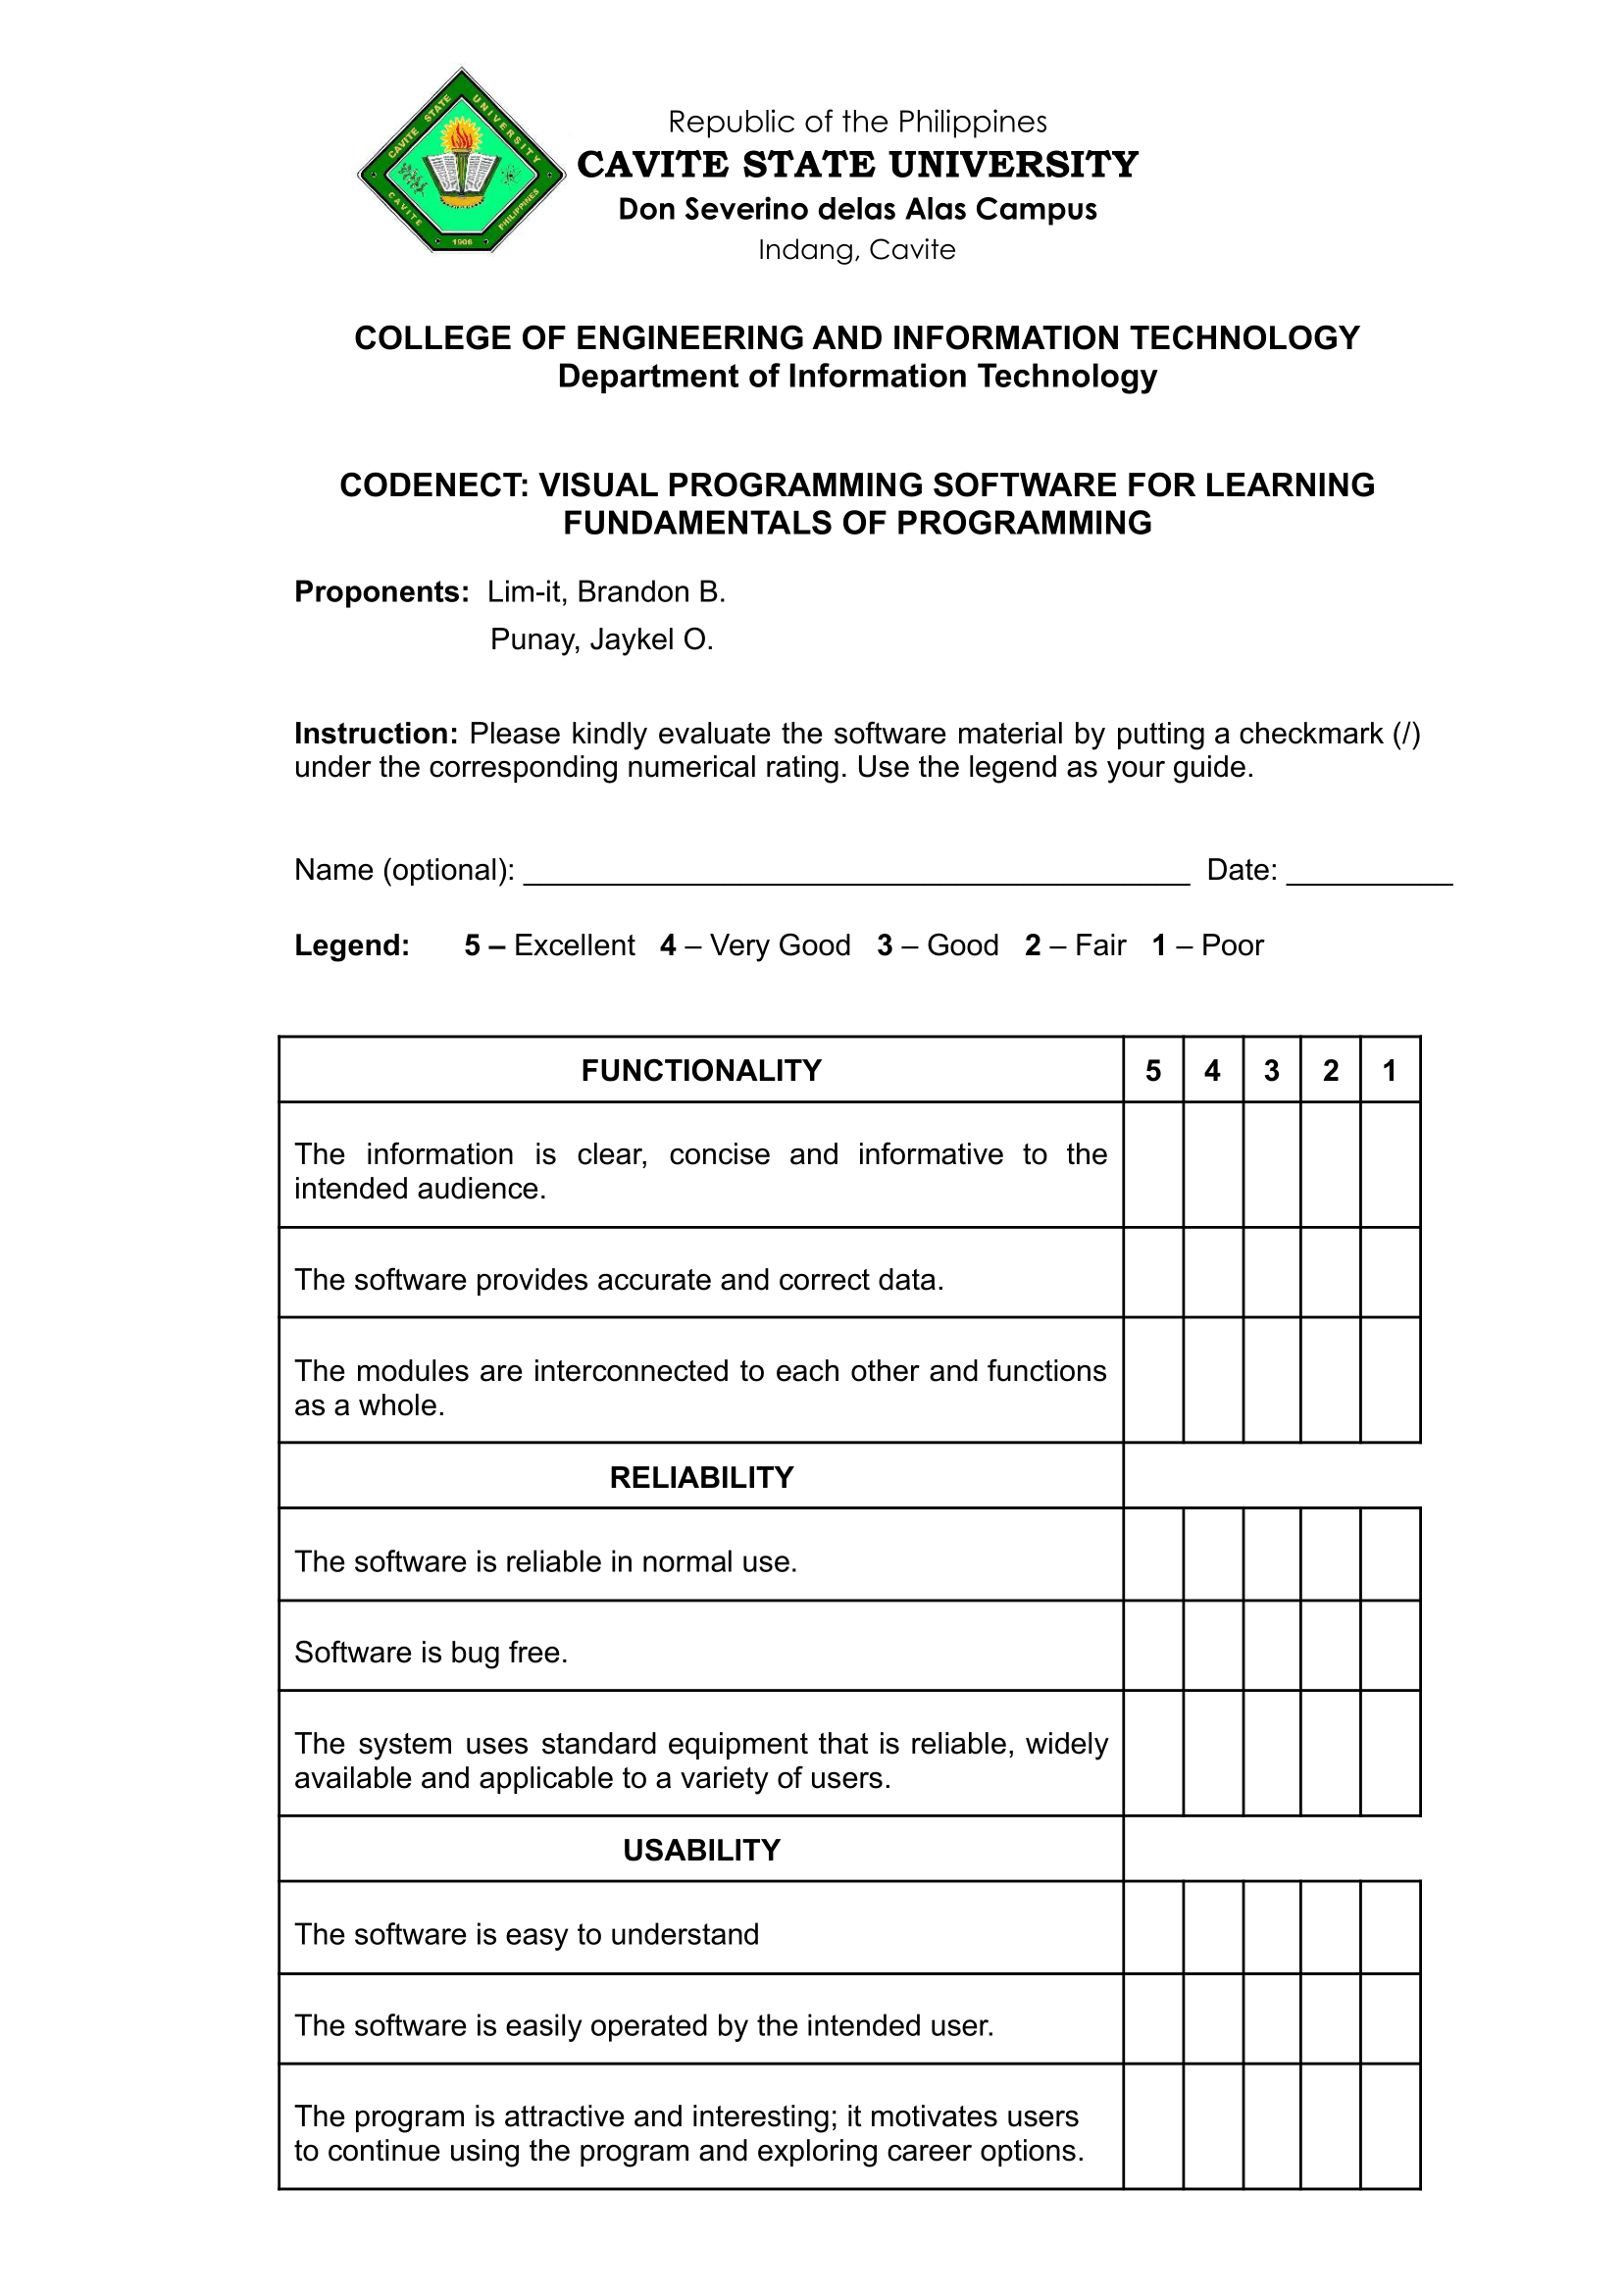
\includegraphics[width=\textwidth]{figures/tech_eval_form.png}
	 \caption[]{Technical Evaluation Form}
	 \label{fig:tech_eval_form}
\end{figure}

\clearpage
\null\vfill
\begin{figure}[H]
	 \centering
	 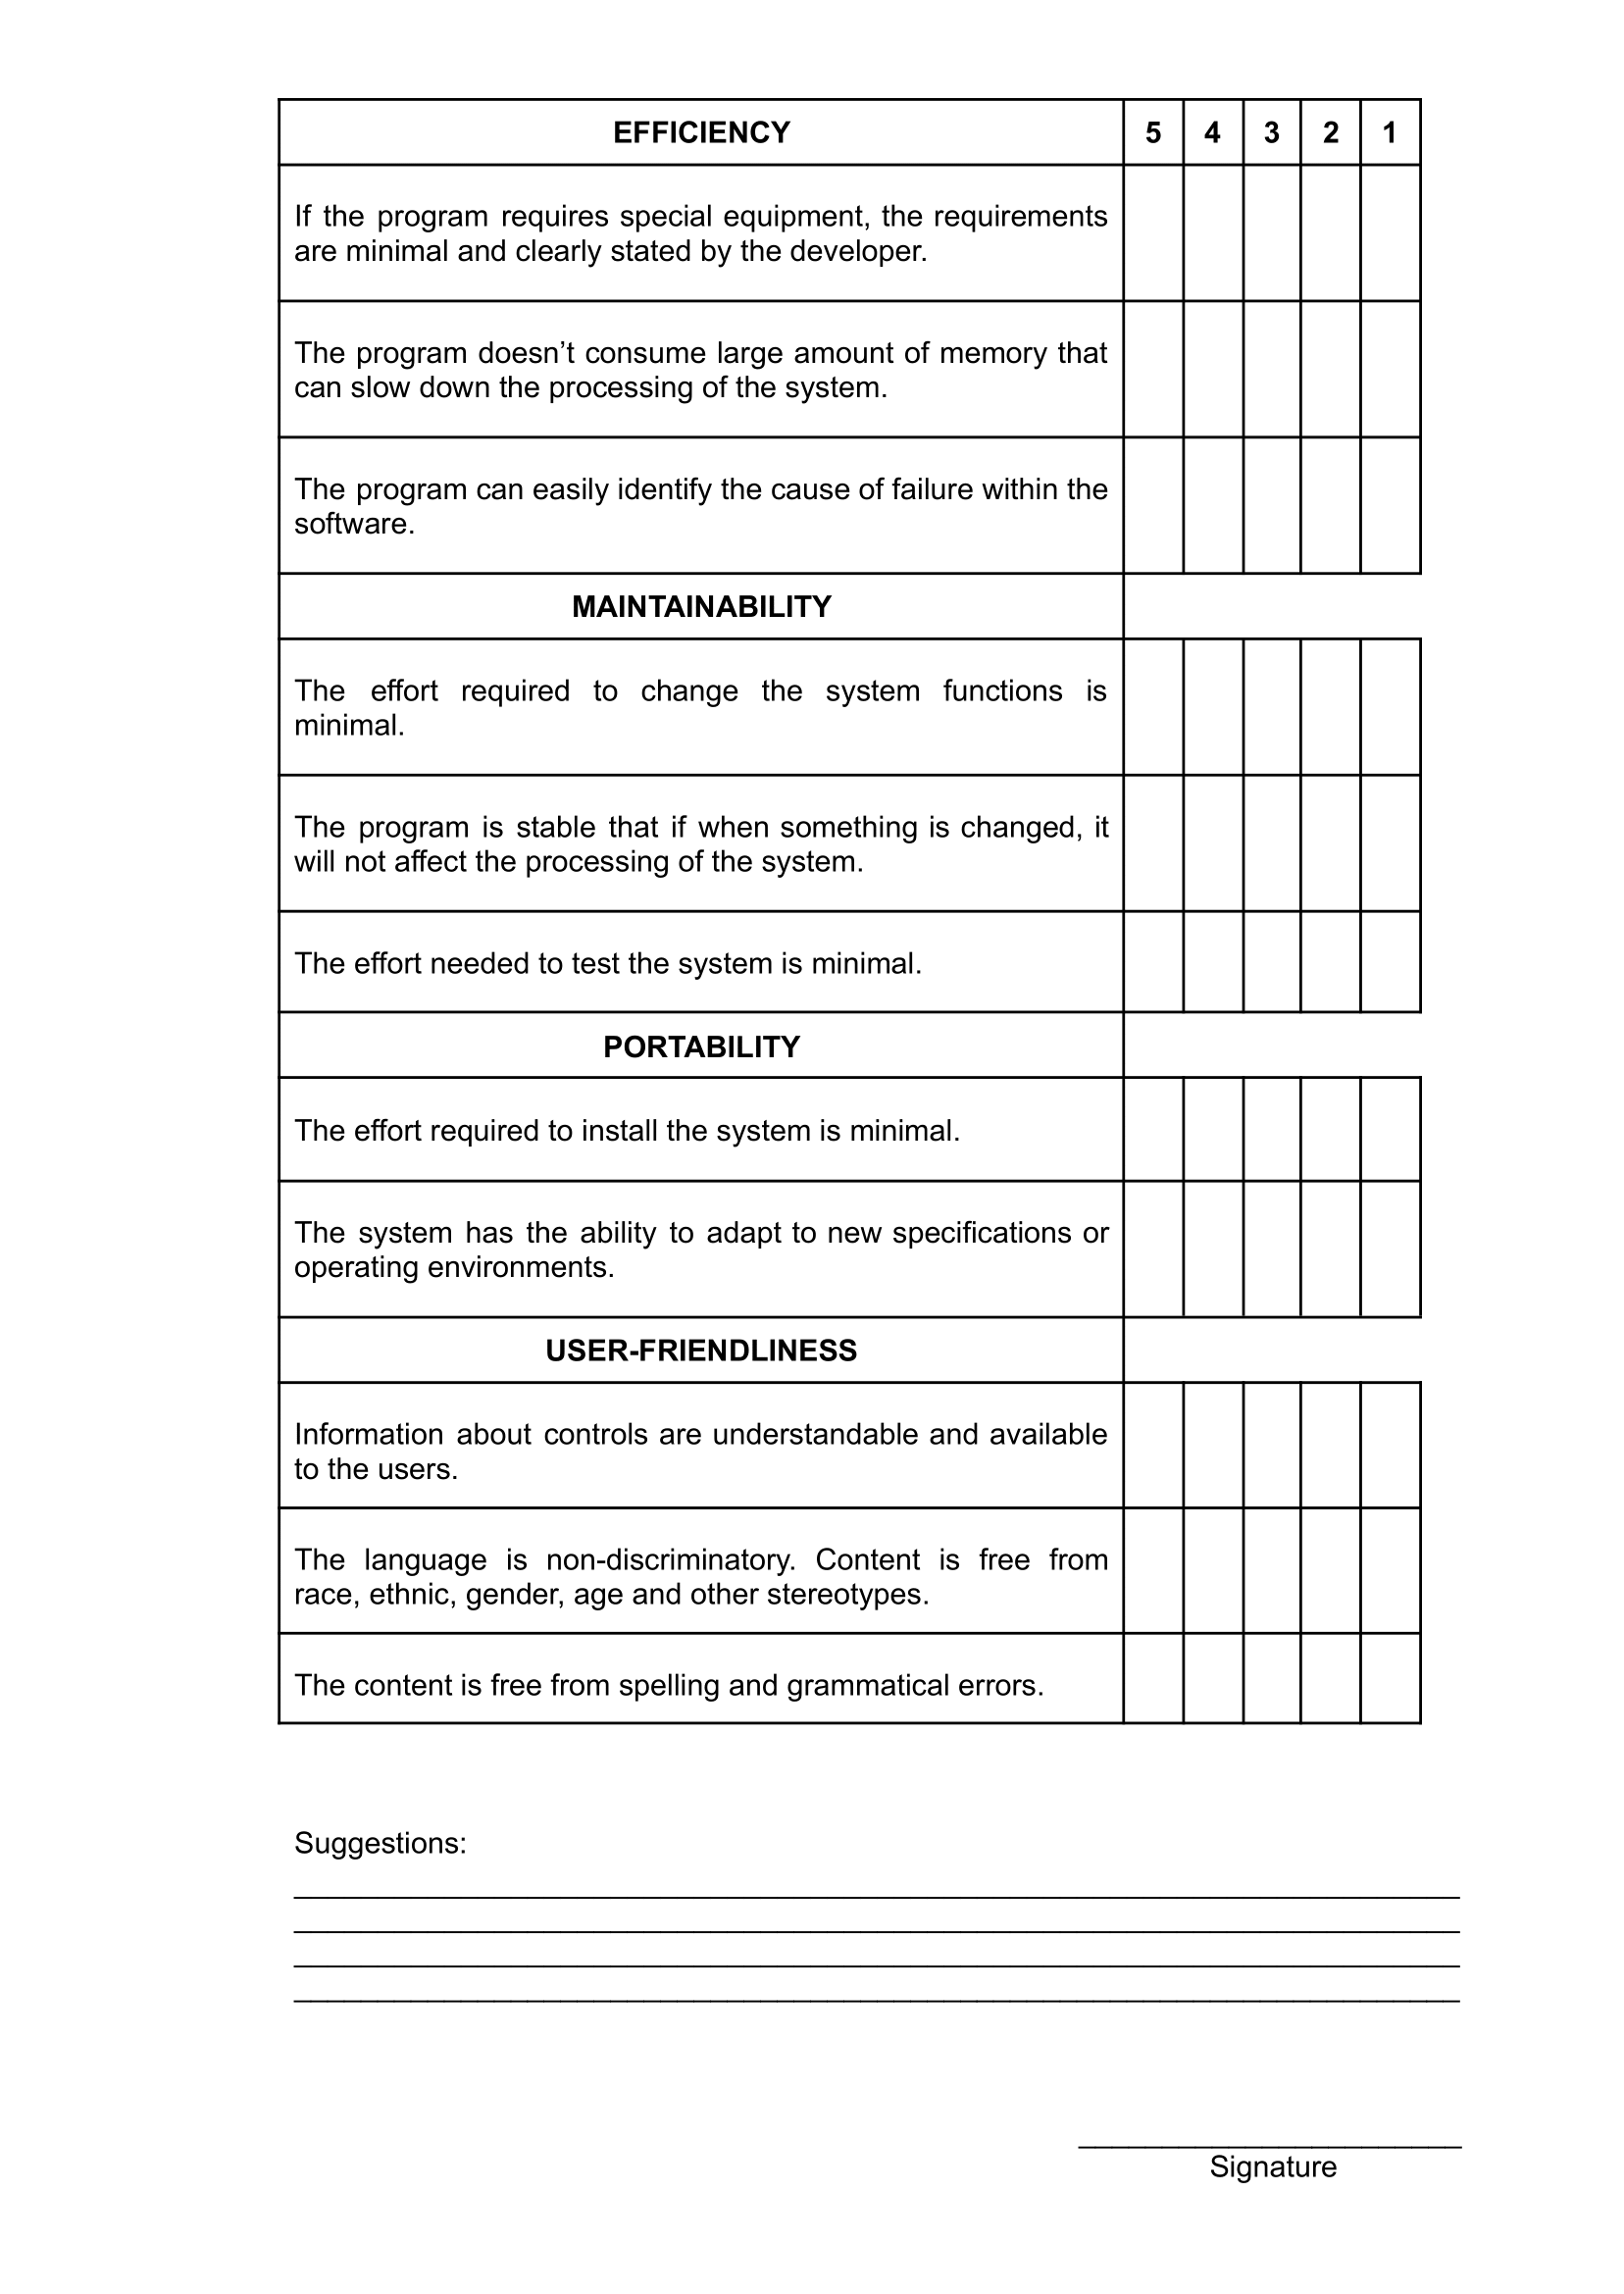
\includegraphics[width=\textwidth]{figures/tech_eval_form_2.png}
	 \label{fig:tech_eval_form2}
\end{figure}

		% \appfig{Graphical Representation of Data}
\renewcommand{\figurename}{Appendix Figure}
\clearpage
\null\vfill
\appendixdata{1}
\appfig{Graphical representation of the course and strand of the respondents}
\label{dataresults1}
\vfill
\appendixdata{2}
\appfig{Graphical representation of the grade/year level of the respondents}
\label{dataresults2}
\vfill

\clearpage
\null\vfill
\appendixdata{3}
\appfig{Graphical representation of the desired technology field of the respondents}
\label{dataresults3}
\vfill
\appendixdata{4}
\appfig{Graphical representation of knowing programming pre-college of the respondents}
\label{dataresults4}
\vfill

\clearpage
\null\vfill
\appendixdata{5}
\appfig{Graphical representation of the years programming of the respondents}
\label{dataresults5}
\vfill
\appendixdata{6}
\appfig{Graphical representation of the languages comfortable with of the respondents}
\label{dataresults6}
\vfill

\clearpage
\null\vfill
\appendixdata{7}
\appfig{Graphical representation of the best learning method of the respondents}
\label{dataresults7}
\vfill
\appendixdata{8}
\appfig{Graphical representation of the hard to learn in programming of the respondents}
\label{dataresults8}
\vfill

\clearpage
\null\vfill
\appendixdata{9}
\appfig{Graphical representation of the text-editing tool used of the respondents}
\label{dataresults9}
\vfill
\appendixdata{10}
\appfig{Graphical representation of the preferred alternative learning method of the respondents}
\label{dataresults10}
\vfill

\clearpage
\null\vfill
\appendixdata{11}
\appfig{Graphical representation of the text editors' usage ease of the respondents}
\label{dataresults11}
\vfill
\appendixdata{12}
\appfig{Graphical representation of the programming fundamentals understanding of the respondents}
\label{dataresults12}
\vfill

\clearpage
\null\vfill
\appendixdata{13}
\appfig{Graphical representation of the programming fundamentals assessment of the respondents}
\label{dataresults13}
\vfill


		% \subsection*{APPENDIX C} \label{ishikawadiagrams}
		% \subsubsection*{Ishikawa Diagrams}
		\clearpage
		\null\vfill
		\appfig{Ishikawa Diagram}
		\begin{figure}[H]
			\centering
			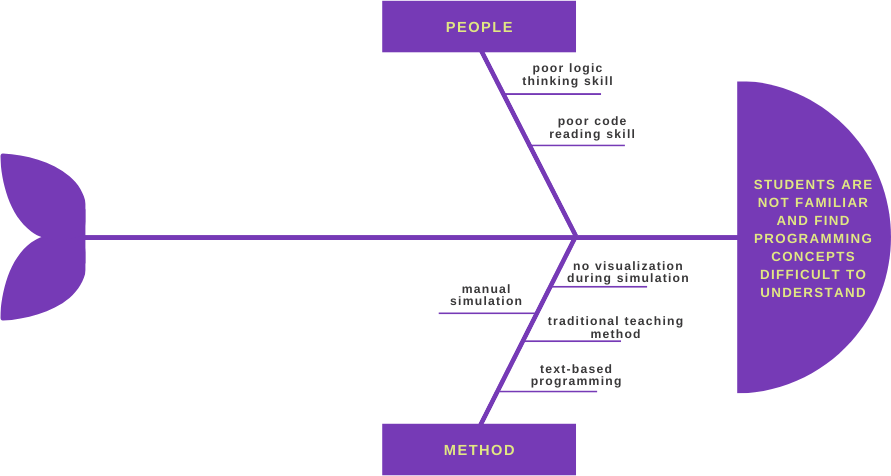
\includegraphics[width=0.8\textheight,angle=90]{figures/fishbone1.png}
			% \caption[Ishikawa Diagram 1]{Fishbone diagram of the students are not familiar and find
			% programming concepts difficult to understand}
			\label{fig:fishbone1}
		\end{figure}
		\appfig{Fishbone diagram of the students not familiar and find programming concepts difficult to understand}
		\label{fishbone1}
		\vfill

		\clearpage
		\null\vfill
		\begin{figure}[H]
			\centering
			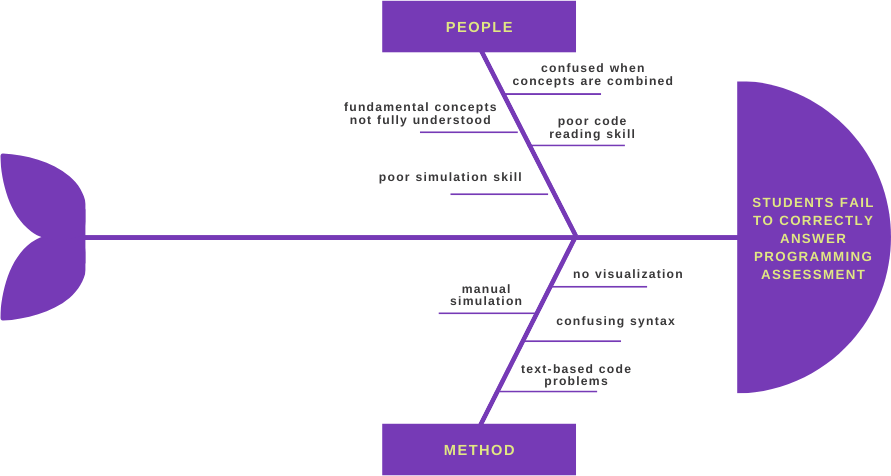
\includegraphics[width=0.8\textheight,angle=90]{figures/fishbone2.png}
			% \caption[Ishikawa Diagram 2]{Fishbone diagram of the students fail to correctly answer programming
			% assessment}
			\label{fig:fishbone2}
		\end{figure}
		\appfig{Fishbone diagram of the students incorrect answer to programming assessment}
		\label{fishbone2}
		\vfill

		\clearpage
		\null\vfill
		\begin{figure}[H]
			\centering
			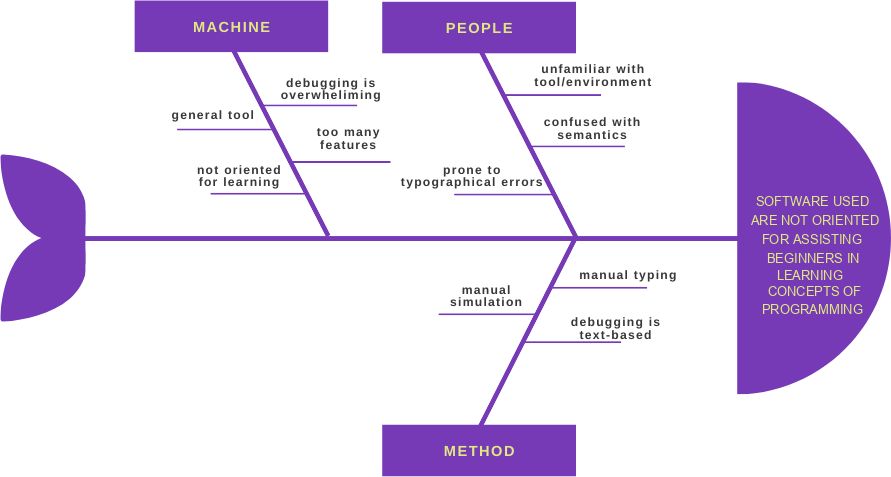
\includegraphics[width=0.8\textheight,angle=90]{figures/fishbone3.png}
			% \caption[Ishikawa Diagram 3]{Fishbone diagram of the tool for programming not effective for
			% learning}
			\label{fig:fishbone3}
		\end{figure}
		\appfig{Fishbone diagram of the tool for programming not effective for learning}
		\label{fishbone3}
		\vfill

		% \appendix
		% \subsection*{APPENDIX D} \label{appendixc}
		% \subsubsection*{Context Diagram (Manual)} \label{contextdiagrammanual}
		\clearpage
		\null\vfill
		% \app{Context Diagram}
		\captionsetup[figure]{list=no}
		\begin{figure}[H]
			\centering
			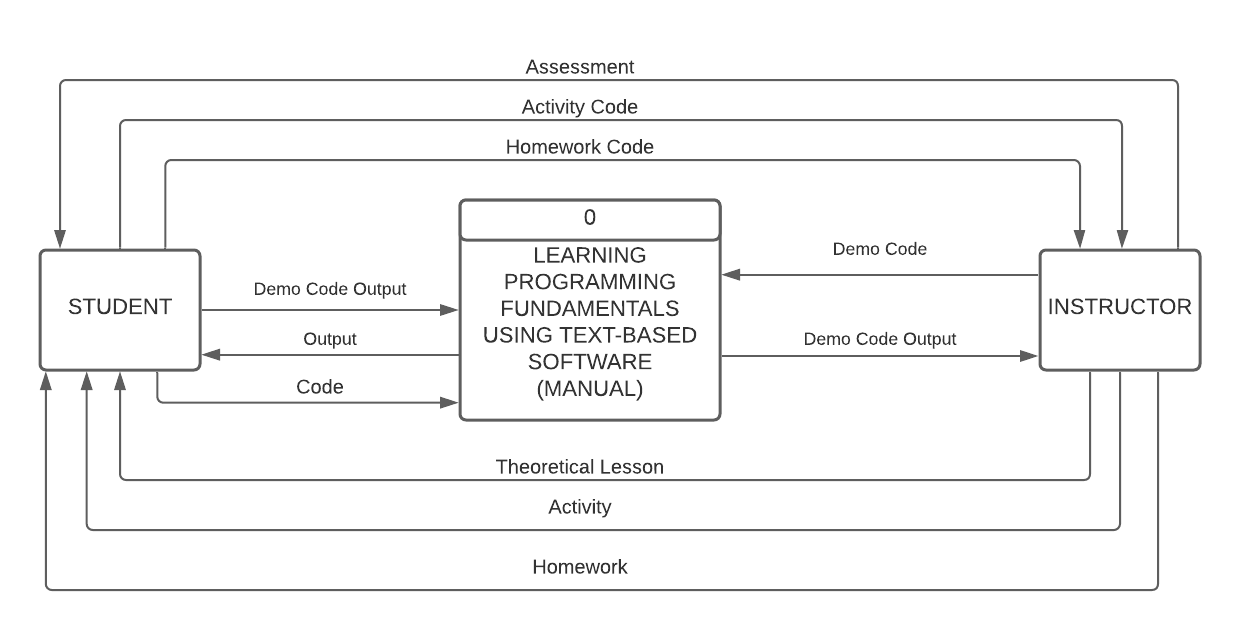
\includegraphics[width=\textwidth]{figures/context_diagram_manual.png}
			\caption{}
			\label{fig:context_diagram_manual}
		\end{figure}
		\appfig{Context Diagram of Existing System}
		\vfill

		% \subsubsection*{Context Diagram} \label{contextdiagram}
		\begin{figure}[H]
			\centering
			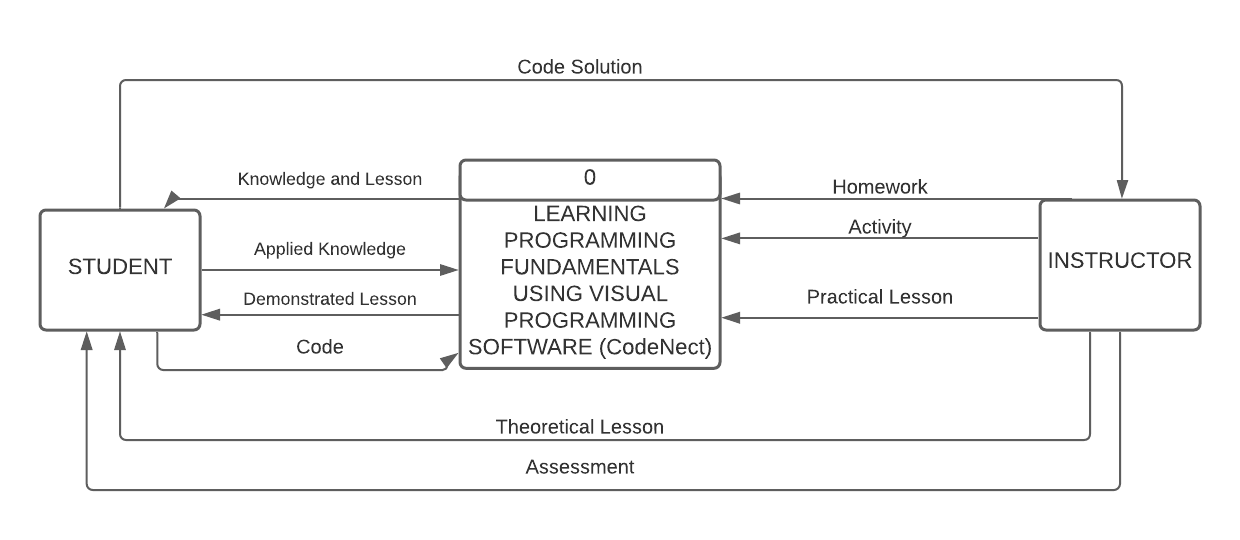
\includegraphics[width=\textwidth]{figures/context_diagram.png}
			\caption{}
			\label{fig:context_diagram}
		\end{figure}
		\appfig{Context Diagram of Proposed System}
		\vfill

		% \subsection*{APPENDIX E} \label{ganttchart}
		% \subsubsection*{Gantt Chart}
		% \begin{figure}[H]
		% 	\centering
		% 	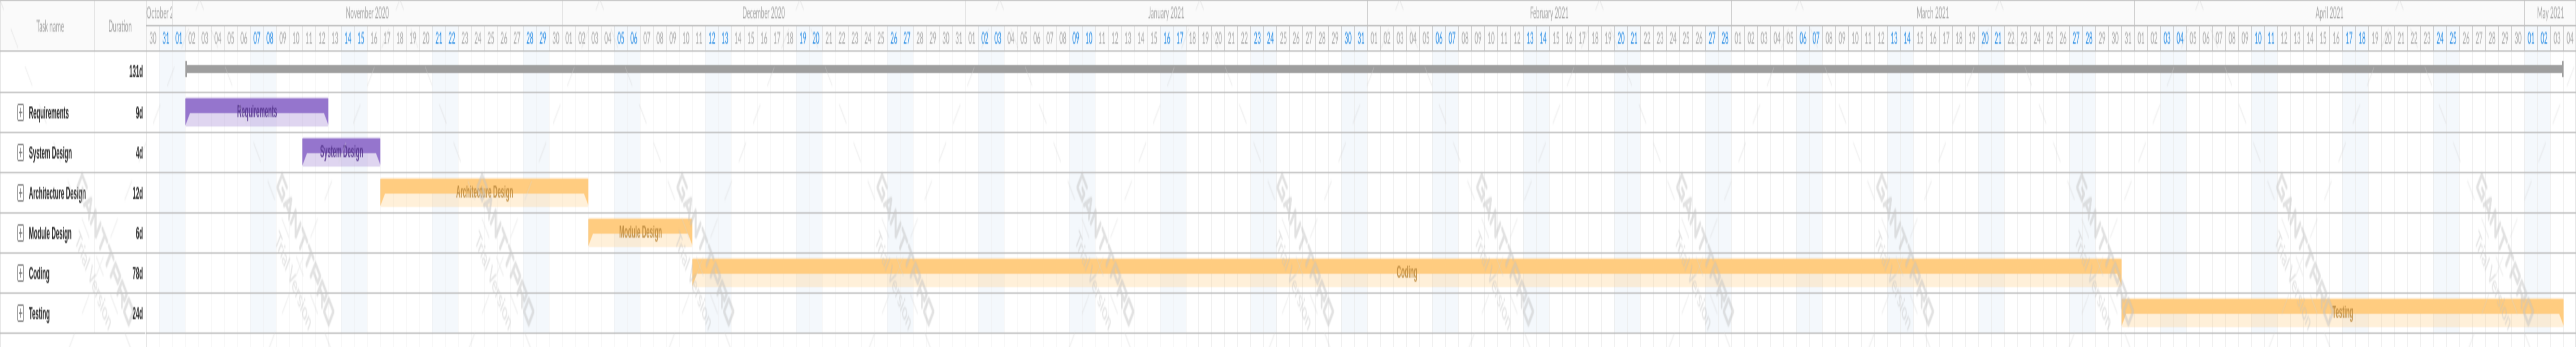
\includegraphics[width=0.8\textheight,angle=90]{figures/gantt_chart.png}
		% 	\caption[Gantt Chart]{Gantt Chart of the Development of CodeNect}
		% 	\label{fig:gantt_chart}
		% \end{figure}

		% \app{Gantt Chart}
		\begin{sidewaysfigure}
			\centering
			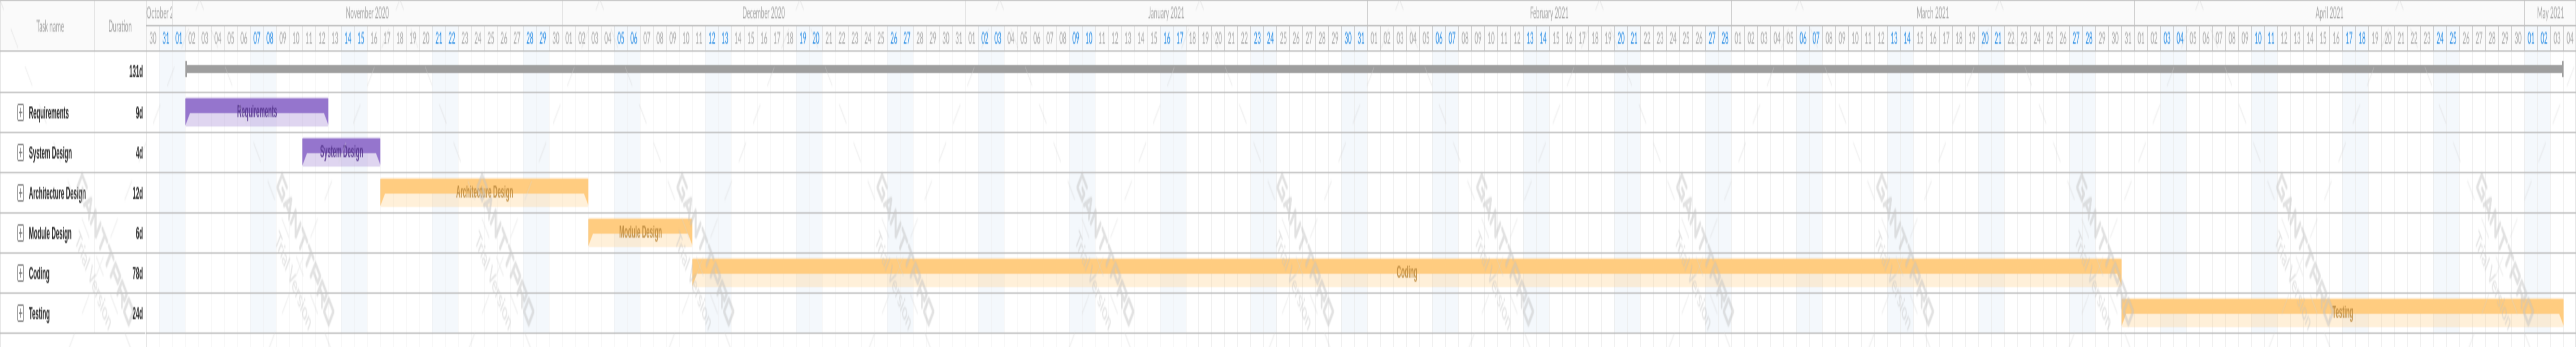
\includegraphics[width=\textwidth,height=\textheight,keepaspectratio]{figures/gantt_chart.png}
			\caption{}
			\label{fig:gantt_chart}
			\appfig{Gantt Chart of the Development of CodeNect}
		\end{sidewaysfigure}
		\vfill

		\clearpage
		\null\vfill
		% \subsection*{APPENDIX F} \label{theoreticalframework}
		% \subsubsection*{Theoretical Framework}
		% \app{Theoretical Framework}
		\begin{figure}[H]
			\centering
			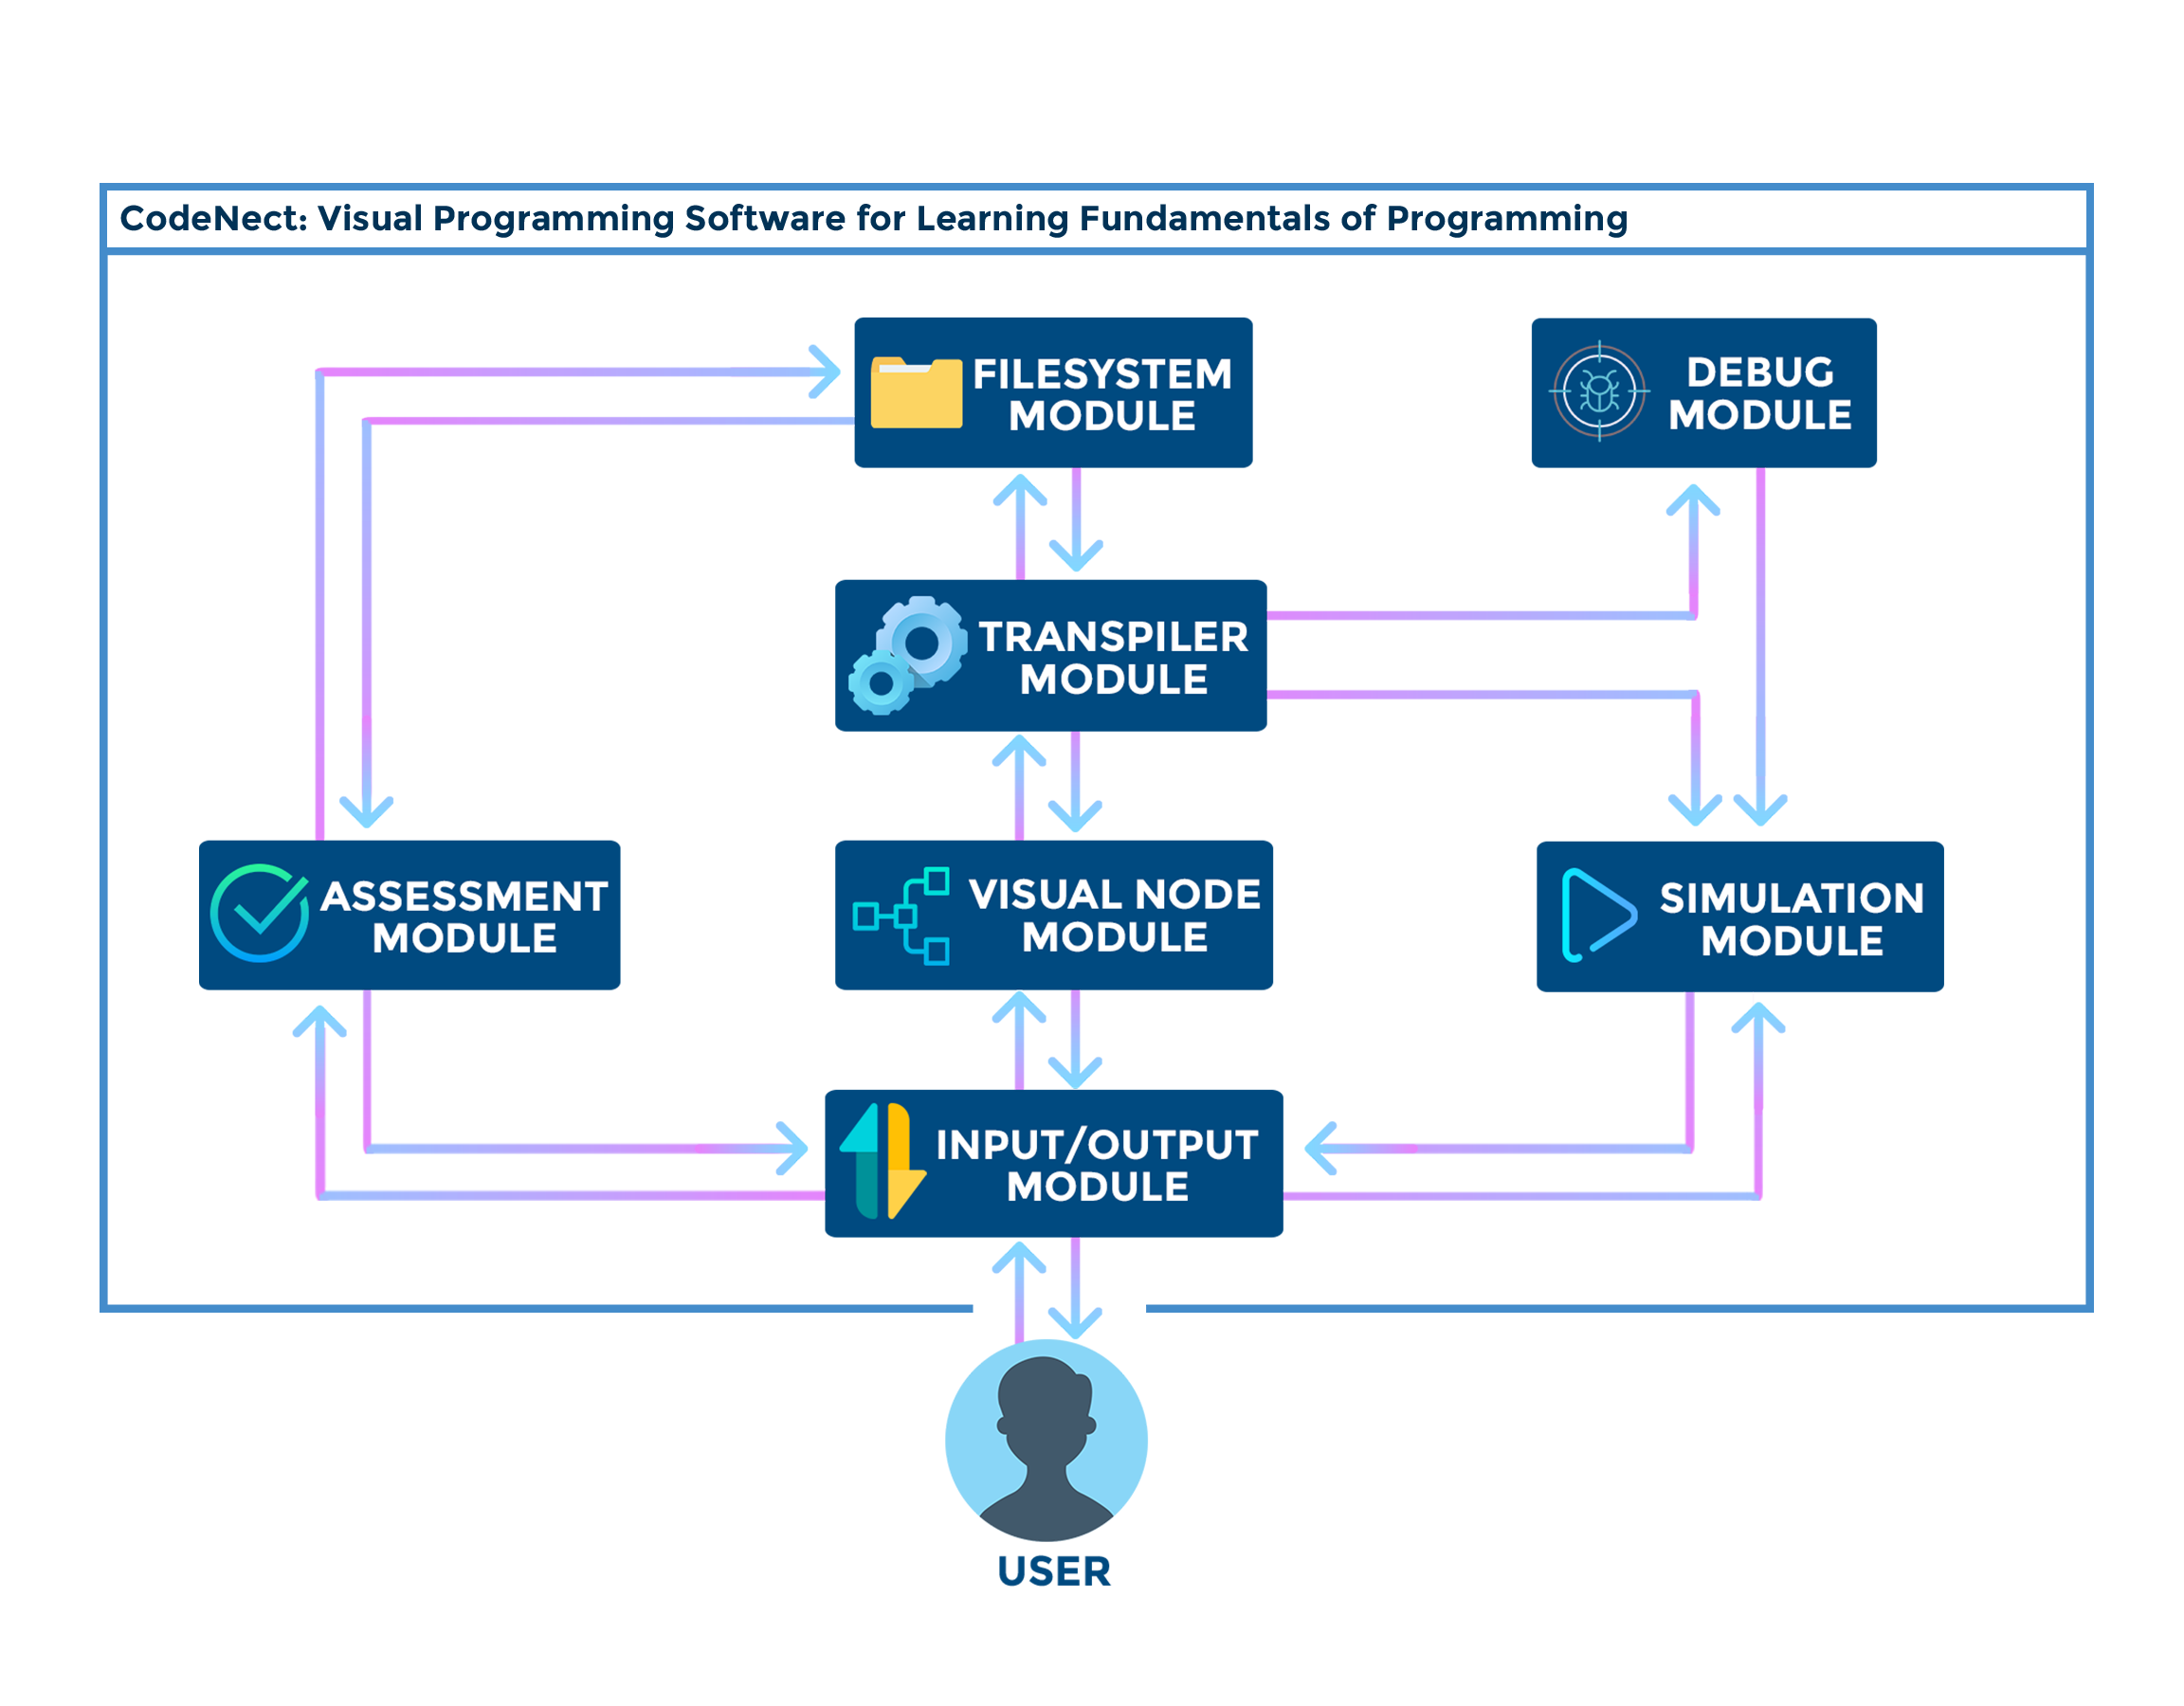
\includegraphics[width=\textwidth]{figures/theoretical_framework.png}
			\caption{}
			\label{fig:theoretical_framework}
		\end{figure}
		\appfig{Theoretical Framework of CodeNect: Visual Programming Software for Learning Fundamentals of Programming}
		\vfill

		\clearpage
\app{Unit Testing}
\textbf{UNIT TESTING SHEET}
\leavevmode\\
\begin{flushleft}
	\textbf{Proponents: LIM-IT, BRANDON B., PUNAY, JAYKEL O.}
	\leavevmode\\
	Date: May, 2021
\end{flushleft}

% Please add the following required packages to your document preamble:
% \usepackage{longtable}
% Note: It may be necessary to compile the document several times to get a multi-page table to line up properly
\begin{longtable}[c]{|l|c|c|}
\hline
\multicolumn{1}{|c|}{\textbf{FUNCTIONALITY}} & \textbf{PASSED/FAILED} & \textbf{REMARKS} \\ \hline
\endfirsthead
%
\endhead
%
\multicolumn{3}{|l|}{\textbf{Visual Nodes Module}}                                       \\ \hline
1. Create Nodes                              & PASSED                 & OK               \\ \hline
2. Edit Nodes                                & PASSED                 & OK               \\ \hline
3. Delete Nodes                              & PASSED                 & OK               \\ \hline
4. Connect Nodes                             & PASSED                 & OK               \\ \hline
5. Process Logic                             & PASSED                 & OK               \\ \hline
\multicolumn{3}{|l|}{\textbf{Filesystem Module}}                                         \\ \hline
1. Create Project                            & PASSED                 & OK               \\ \hline
2. Open/Load Project                         & PASSED                 & OK               \\ \hline
3. Save Project                              & PASSED                 & OK               \\ \hline
4. Linux platform compatibility              & PASSED                 & OK               \\ \hline
5. Windows platform compatibility            & PASSED                 & OK               \\ \hline
\multicolumn{3}{|l|}{\textbf{Input/Output Module}}                                       \\ \hline
1. Keyboard compatibility                    & PASSED                 & OK               \\ \hline
2. Mouse Compatibility                       & PASSED                 & OK               \\ \hline
3. User interaction                          & PASSED                 & OK               \\ \hline
4. Feedback/Response to User                 & PASSED                 & OK               \\ \hline
\multicolumn{3}{|l|}{\textbf{Debug Module}}                                              \\ \hline
1. Detect warning/error                      & PASSED                 & OK               \\ \hline
2. Identify cause of warning/error           & PASSED                 & OK               \\ \hline
3. Find cause of warning/error               & PASSED                 & OK               \\ \hline
4. Display warning/error                     & PASSED                 & OK               \\ \hline
\multicolumn{3}{|l|}{\textbf{Simulation Module}}                                         \\ \hline
1. Forward iterate control                   & PASSED                 & OK               \\ \hline
2. Backward iterate control                  & PASSED                 & OK               \\ \hline
3. Automatic iteration control               & PASSED                 & OK               \\ \hline
4. Timer for iteration control               & PASSED                 & OK               \\ \hline
5. Stop/Reset iteration control              & PASSED                 & OK               \\ \hline
\multicolumn{3}{|l|}{\textbf{Transpiler Module}}                                         \\ \hline
1. Transpile visual code to C language       & PASSED                 & OK               \\ \hline
2. Compile transpiled code                   & PASSED                 & OK               \\ \hline
3. Run compiled code                         & PASSED                 & OK               \\ \hline
4. Linux compatibility                       & PASSED                 & OK               \\ \hline
5. Windows compatibility                     & PASSED                 & OK               \\ \hline
\multicolumn{3}{|l|}{\textbf{Assessment Module}}                                         \\ \hline
1. Display assessment                        & PASSED                 & OK               \\ \hline
2. Submit code for assessment                & PASSED                 & OK               \\ \hline
3. Compare submitted with expected output    & PASSED                 & OK               \\ \hline
4. Calculate score                           & PASSED                 & OK               \\ \hline
5. Show mistakes                             & PASSED                 & OK               \\ \hline
\caption[Unit Testing]{Unit Testing}
\end{longtable}

		\clearpage
\app{Integration Testing}
\textbf{INTEGRATION TESTING SHEET}
\leavevmode\\
\begin{flushleft}
	\textbf{Proponents: LIM-IT, BRANDON B., PUNAY, JAYKEL O.}
	\leavevmode\\
	Date: May 21, 2021
\end{flushleft}

% Please add the following required packages to your document preamble:
% \usepackage{multirow}
% \usepackage{longtable}
% Note: It may be necessary to compile the document several times to get a multi-page table to line up properly
\begin{longtable}[c]{|c|l|c|}
\hline
\textbf{MODULE}                               & \multicolumn{1}{c|}{\textbf{FUNCTIONALITY}} & \textbf{REMARKS} \\ \hline
\endfirsthead
%
\endhead
%
\multirow{5}{*}{\textbf{Visual Nodes Module}} & 1. Create Nodes                             & OK               \\ \cline{2-3} 
                                              & 2. Edit Nodes                               & OK               \\ \cline{2-3} 
                                              & 3. Delete Nodes                             & OK               \\ \cline{2-3} 
                                              & 4. Connect Nodes                            & OK               \\ \cline{2-3} 
                                              & 5. Process Logic                            & OK               \\ \hline
\multirow{5}{*}{\textbf{Filesystem Module}}   & 1. Create Project                           & OK               \\ \cline{2-3} 
                                              & 2. Open/Load Project                        & OK               \\ \cline{2-3} 
                                              & 3. Save Project                             & OK               \\ \cline{2-3} 
                                              & 4. Linux platform compatibility             & OK               \\ \cline{2-3} 
                                              & 5. Windows platform compatibility           & OK               \\ \hline
\multirow{4}{*}{\textbf{Input/Output Module}} & 1. Keyboard compatibility                   & OK               \\ \cline{2-3} 
                                              & 2. Mouse Compatibility                      & OK               \\ \cline{2-3} 
                                              & 3. User interaction                         & OK               \\ \cline{2-3} 
                                              & 4. Feedback/Response to User                & OK               \\ \hline
\multirow{4}{*}{\textbf{Debug Module}}        & 1. Detect warning/error                     & OK               \\ \cline{2-3} 
                                              & 2. Identify cause of warning/error          & OK               \\ \cline{2-3} 
                                              & 3. Find cause of warning/error              & OK               \\ \cline{2-3} 
                                              & 4. Display warning/error                    & OK               \\ \hline
\multirow{5}{*}{\textbf{Simulation Module}}   & 1. Forward iterate control                  & OK               \\ \cline{2-3} 
                                              & 2. Backward iterate control                 & OK               \\ \cline{2-3} 
                                              & 3. Automatic iteration control              & OK               \\ \cline{2-3} 
                                              & 4. Timer for iteration control              & OK               \\ \cline{2-3} 
                                              & 5. Stop/Reset iteration control             & OK               \\ \hline
\multirow{5}{*}{\textbf{Transpiler Module}}   & 1. Transpile visual code to C language      & OK               \\ \cline{2-3} 
                                              & 2. Compile transpiled code                  & OK               \\ \cline{2-3} 
                                              & 3. Run compiled code                        & OK               \\ \cline{2-3} 
                                              & 4. Linux compatibility                      & OK               \\ \cline{2-3} 
                                              & 5. Windows compatibility                    & OK               \\ \hline
\multirow{5}{*}{\textbf{Assessment Module}}   & 1. Display assessment                       & OK               \\ \cline{2-3} 
                                              & 2. Submit code for assessment               & OK               \\ \cline{2-3} 
                                              & 3. Compare submitted with expected output   & OK               \\ \cline{2-3} 
                                              & 4. Calculate score                          & OK               \\ \cline{2-3} 
                                              & 5. Show mistakes                            & OK               \\ \hline
\caption[Integration Testing]{Integration Testing}
\end{longtable}

		\clearpage
\app{Profile of Respondents}
\leavevmode\\

\begin{longtable}[c]{|c|c|}
\hline
\textbf{Respondents} & \textbf{Number} \\ \hline
\endfirsthead
%
\endhead
%
Students (BSIT/BSCS) & 12              \\ \hline
IT Professionals     & 10              \\ \hline
\textbf{Total}       & \textbf{22}     \\ \hline
\end{longtable}

\begin{longtable}[c]{|l|l|l|l|l|}
\hline
\multicolumn{1}{|c|}{\textbf{Name}}    & \multicolumn{1}{c|}{\textbf{E-Mail Address}} & \multicolumn{1}{c|}{\textbf{Designation/Rank}} & \multicolumn{1}{c|}{\textbf{Institution}} & \multicolumn{1}{c|}{\textbf{Educational Attainment}} \\ \hline
\endfirsthead
%
\endhead
%
(not mentioned due to confidentiality) & auahdark687291@gmail.com                     & Software Engineer and Game Developer           & Hasanuddin University                     & Information Systems                                  \\ \hline
(not mentioned due to confidentiality) & thereal.alex.b@gmail.com                     & System Programmer and Lead Programmer          & Syntacore                                 & Computer Science                                     \\ \hline
Fort Bautista                          & febhd0120@gmail.com                          & Web Developer                                  & Snipesoft Ltd                             & Information Technology                               \\ \hline
Michael Gelvez                         & gelvezmichael@yahoo.com                      & Web Developer                                  & Straight Login                            & Information Technology                               \\ \hline
Ronalyn De Guzman Rioflorido           & ronrioflorido2@gmail.com                     & Web Developer and Trading Staff                & Fatec Corporation                         & Information Technology                               \\ \hline
John Eros Puyo                         & johnerospuyo21@gmail.com                     & Instructor                                     & Philippine Christian University           & MIS                                                  \\ \hline
Ralph Waldo Candaza                    & rccandaza@up.edu.ph                          & Web Developer                                  & Stratpoint                                & Computer Science                                     \\ \hline
Jaypee Galang                          & jaypeegalang27@gmail.com                     & Web Developer and Instructor                   & ISDC                                      & Information Technology                               \\ \hline
Cyril Elijah Maurino                   & cyrilelijahaurino@gmail.com                  & Software Developer                             & Controtek Solutions                       & Computer Science                                     \\ \hline
Conrad Reyes                           & conradreyes123@gmail.com                     & Web Developer and Game Developer               & Shopify                                   & Information Technology                               \\ \hline
Jerald Vidallo                         & jerald.vidallo@cvsu.edu.ph                   & IT Student                                     & Cavite State University                   &                                                      \\ \hline
Ron Tseytlin                           & ronts390@gmail.com                           & CS Student                                     & Ben Gurion University                     &                                                      \\ \hline
Angelo Mari Paredes                    & angelomariparedes@gmail.com                  & STEM Student                                   & Luis Y. Ferrer Jr. Senior High School     &                                                      \\ \hline
Ian Virgil Plaus                       & mitoplaus@gmail.com                          & CPE Student                                    & De La Salle University                    &                                                      \\ \hline
Edward Conception                      & edward.concepcion@cvsu.edu.ph                & IT Student                                     & Cavite State University                   &                                                      \\ \hline
Marie Joy Musa                         & mariejoy.musa@cvsu.edu.ph                    & IT Student                                     & Cavite State University                   &                                                      \\ \hline
Marvin Recto                           & marvin.recto@cvsu.edu.ph                     & IT Student                                     & Cavite State University                   &                                                      \\ \hline
Lmarl Saria                            & lmarlsaria21@gmail.com                       & IT Student                                     & Cavite State University                   &                                                      \\ \hline
Ren Antonio                            & reneantonio.dimabogte@cvsu.edu.ph            & IT Student                                     & Cavite State University                   &                                                      \\ \hline
Rhealyn Villar                         & rhealynvillar@gmail.com                      & IT Student                                     & Cavite State University                   &                                                      \\ \hline
Jingkie Lagarde                        & jingkie.lagarde@cvsu.edu.ph                  & IT Student                                     & Cavite State University                   &                                                      \\ \hline
Jaymark Abulencia                      & jaymark.abulencia@cvsu.edu.ph                & IT Student                                     & Cavite State University                   &                                                      \\ \hline
\end{longtable}

		\clearpage
\app{Frequence Distribution Table}
\textbf{Technical}
\leavevmode\\
% FUNCTIONALITY
\begin{longtable}[c]{|l|c|c|c|c|c|c|c|l|c|c|c|}
\hline
\multicolumn{1}{|c|}{\multirow{2}{*}{\textbf{Indicator}}}                                                                  & \multicolumn{2}{c|}{\textbf{Excellent}} & \multicolumn{2}{c|}{\textbf{Very Good}} & \multicolumn{2}{c|}{\textbf{Good}} & \multicolumn{3}{c|}{\textbf{Fair}}                 & \multicolumn{2}{c|}{\textbf{Total}} \\ \cline{2-12} 
\multicolumn{1}{|c|}{}                                                                                                     & \textbf{f}         & \textbf{\%}        & \textbf{f}         & \textbf{\%}        & \textbf{f}      & \textbf{\%}      & \multicolumn{2}{c|}{\textbf{f}} & \textbf{\%}      & \textbf{f}       & \textbf{\%}      \\ \hline
\endfirsthead
%
\endhead
%
\begin{tabular}[c]{@{}l@{}}The information is clear,\\ concise, and informative\\ to the intended\\ audience.\end{tabular} & 4                  & 40\%               & 3                  & 30\%               & 2               & 20\%             & \multicolumn{2}{c|}{1}          & 10\%             & 10               & 100\%            \\ \hline
\begin{tabular}[c]{@{}l@{}}The software provides\\ accurate and correct\\ data.\end{tabular}                               & 5                  & 50\%               & 4                  & 40\%               & 1               & 10\%             & \multicolumn{2}{c|}{}           &                  & 10               & 100\%            \\ \hline
\begin{tabular}[c]{@{}l@{}}The modules areinterconnected with\\ each other and\\ functions as a whole.\end{tabular}        & 7                  & 70\%               & 2                  & 20\%               & 1               & 10\%             & \multicolumn{2}{c|}{}           &                  & 10               & 100\%            \\ \hline
\caption{Frequency Distribution of Scores on Functionality (Technical)}
\label{table:ft_t_functionality}\\
\end{longtable}

% RELIABILITY
\begin{longtable}[c]{|l|c|c|c|c|c|c|c|l|c|c|c|}
\hline
\multicolumn{1}{|c|}{\multirow{2}{*}{\textbf{Indicator}}}                                                                                                   & \multicolumn{2}{c|}{\textbf{Excellent}} & \multicolumn{2}{c|}{\textbf{Very Good}} & \multicolumn{2}{c|}{\textbf{Good}} & \multicolumn{3}{c|}{\textbf{Fair}}                 & \multicolumn{2}{c|}{\textbf{Total}} \\ \cline{2-12} 
\multicolumn{1}{|c|}{}                                                                                                                                      & \textbf{f}         & \textbf{\%}        & \textbf{f}         & \textbf{\%}        & \textbf{f}      & \textbf{\%}      & \multicolumn{2}{c|}{\textbf{f}} & \textbf{\%}      & \textbf{f}       & \textbf{\%}      \\ \hline
\endfirsthead
%
\endhead
%
\begin{tabular}[c]{@{}l@{}}The software is reliable\\ in normal use\end{tabular}                                                                            & 3                  & 30\%               & 5                  & 50\%               & 1               & 10\%             & \multicolumn{2}{c|}{1}          & 10\%             & 10               & 100\%            \\ \hline
Software is bug free.                                                                                                                                       & 2                  & 20\%               & 4                  & 40\%               & 3               & 30\%             & \multicolumn{2}{c|}{1}          & 10\%             & 10               & 100\%            \\ \hline
\begin{tabular}[c]{@{}l@{}}The system uses\\ standard equipment that\\ is reliable, widely\\ available and applicable\\ to a variety of users.\end{tabular} & 4                  & 40\%               & 5                  & 50\%               & 1               & 10\%             & \multicolumn{2}{c|}{}           &                  & 10               & 100\%            \\ \hline
\caption{Frequency Distribution of Scores on Reliability (Technical)}
\label{table:ft_t_reliability}\\
\end{longtable}

% USABLITY
\begin{longtable}[c]{|l|c|c|c|c|c|c|c|l|c|c|c|}
\hline
\multicolumn{1}{|c|}{\multirow{2}{*}{\textbf{Indicator}}}                                                                                                                 & \multicolumn{2}{c|}{\textbf{Excellent}} & \multicolumn{2}{c|}{\textbf{Very Good}} & \multicolumn{2}{c|}{\textbf{Good}} & \multicolumn{3}{c|}{\textbf{Fair}}                 & \multicolumn{2}{c|}{\textbf{Total}} \\ \cline{2-12} 
\multicolumn{1}{|c|}{}                                                                                                                                                    & \textbf{f}         & \textbf{\%}        & \textbf{f}         & \textbf{\%}        & \textbf{f}      & \textbf{\%}      & \multicolumn{2}{c|}{\textbf{f}} & \textbf{\%}      & \textbf{f}       & \textbf{\%}      \\ \hline
\endfirsthead
%
\endhead
%
\begin{tabular}[c]{@{}l@{}}The software is easy to\\ understand.\end{tabular}                                                                                             & 4                  & 40\%               & 3                  & 30\%               & 2               & 20\%             & \multicolumn{2}{c|}{1}          & 10\%             & 10               & 100\%            \\ \hline
\begin{tabular}[c]{@{}l@{}}The software is easily\\ operated by the intended\\ user.\end{tabular}                                                                         & 3                  & 30\%               & 6                  & 60\%               & 1               & 10\%             & \multicolumn{2}{c|}{}           &                  & 10               & 100\%            \\ \hline
\begin{tabular}[c]{@{}l@{}}The program is attractive\\ and interesting; it motivates users to\\ continue using the\\ program and exploring\\ career options.\end{tabular} & 5                  & 50\%               & 3                  & 30\%               & 1               & 10\%             & \multicolumn{2}{c|}{1}           & 10\%                  & 10               & 100\%            \\ \hline
\caption{Frequency Distribution of Scores on Usability (Technical)}
\label{table:ft_t_usability}\\
\end{longtable}

% EFFICIENCY
\begin{longtable}[c]{|l|c|c|c|c|c|c|c|l|c|c|c|}
\hline
\multicolumn{1}{|c|}{\multirow{2}{*}{\textbf{Indicator}}}                                                                                                    & \multicolumn{2}{c|}{\textbf{Excellent}} & \multicolumn{2}{c|}{\textbf{Very Good}} & \multicolumn{2}{c|}{\textbf{Good}} & \multicolumn{3}{c|}{\textbf{Fair}}                 & \multicolumn{2}{c|}{\textbf{Total}} \\ \cline{2-12} 
\multicolumn{1}{|c|}{}                                                                                                                                       & \textbf{f}         & \textbf{\%}        & \textbf{f}         & \textbf{\%}        & \textbf{f}      & \textbf{\%}      & \multicolumn{2}{c|}{\textbf{f}} & \textbf{\%}      & \textbf{f}       & \textbf{\%}      \\ \hline
\endfirsthead
%
\endhead
%
\begin{tabular}[c]{@{}l@{}}If the program requires\\ special equipment, the\\ requirements are minimal\\ and clearly stated by the\\ developer.\end{tabular} & 5                  & 50\%               & 4                  & 40\%               & 1               & 10\%             & \multicolumn{2}{c|}{}           &                  & 10               & 100\%            \\ \hline
\begin{tabular}[c]{@{}l@{}}The program doesn’t\\ consume large amount of\\ memory that can slow\\ down the processing of\\ the system.\end{tabular}          & 6                  & 60\%               & 2                  & 20\%               & 2               & 20\%             & \multicolumn{2}{c|}{}           &                  & 10               & 100\%            \\ \hline
\begin{tabular}[c]{@{}l@{}}The program can easily\\ identify the cause of\\ failure within the\\ software.\end{tabular}                                      & 6                  & 60\%               & 2                  & 20\%               & 2               & 20\%             & \multicolumn{2}{c|}{}           &                  & 10               & 100\%            \\ \hline
\caption{Frequency Distribution of Scores on Efficiency (Technical)}
\label{table:ft_t_efficiency}\\
\end{longtable}

% MAINTAINABILITY
\begin{longtable}[c]{|l|c|c|c|c|c|c|c|l|c|c|c|}
\hline
\multicolumn{1}{|c|}{\multirow{2}{*}{\textbf{Indicator}}}                                                                                                 & \multicolumn{2}{c|}{\textbf{Excellent}} & \multicolumn{2}{c|}{\textbf{Very Good}} & \multicolumn{2}{c|}{\textbf{Good}} & \multicolumn{3}{c|}{\textbf{Fair}}                 & \multicolumn{2}{c|}{\textbf{Total}} \\ \cline{2-12} 
\multicolumn{1}{|c|}{}                                                                                                                                    & \textbf{f}         & \textbf{\%}        & \textbf{f}         & \textbf{\%}        & \textbf{f}      & \textbf{\%}      & \multicolumn{2}{c|}{\textbf{f}} & \textbf{\%}      & \textbf{f}       & \textbf{\%}      \\ \hline
\endfirsthead
%
\endhead
%
\begin{tabular}[c]{@{}l@{}}The effort required to\\ change the system\\ functions is minimal.\end{tabular}                                                & 5                  & 50\%               & 3                  & 30\%               & 2               & 20\%             & \multicolumn{2}{c|}{}           &                  & 10               & 100\%            \\ \hline
\begin{tabular}[c]{@{}l@{}}The program is stable\\ that if when something is\\ changed, it will not affect\\ the processing of the\\ system.\end{tabular} & 5                  & 50\%               & 3                  & 30\%               & 2               & 20\%             & \multicolumn{2}{c|}{}           &                  & 10               & 100\%            \\ \hline
\begin{tabular}[c]{@{}l@{}}The effort needed to test\\ the system is minimal.\end{tabular}                                                                & 4                  & 40\%               & 5                  & 50\%               & 1               & 10\%             & \multicolumn{2}{c|}{}           &                  & 10               & 100\%            \\ \hline
\caption{Frequency Distribution of Scores on Maintainability (Technical)}
\label{table:ft_t_maintainability}\\
\end{longtable}

% PORTABILITY
\begin{longtable}[c]{|l|c|c|c|c|c|c|c|l|c|c|c|}
\hline
\multicolumn{1}{|c|}{\multirow{2}{*}{\textbf{Indicator}}}                                                                          & \multicolumn{2}{c|}{\textbf{Excellent}} & \multicolumn{2}{c|}{\textbf{Very Good}} & \multicolumn{2}{c|}{\textbf{Good}} & \multicolumn{3}{c|}{\textbf{Fair}}                 & \multicolumn{2}{c|}{\textbf{Total}} \\ \cline{2-12} 
\multicolumn{1}{|c|}{}                                                                                                             & \textbf{f}         & \textbf{\%}        & \textbf{f}         & \textbf{\%}        & \textbf{f}      & \textbf{\%}      & \multicolumn{2}{c|}{\textbf{f}} & \textbf{\%}      & \textbf{f}       & \textbf{\%}      \\ \hline
\endfirsthead
%
\endhead
%
\begin{tabular}[c]{@{}l@{}}The effort required to\\ install the system is\\ minimal.\end{tabular}                                  & 8                  & 80\%               & 1                  & 10\%               & 1               & 10\%             & \multicolumn{2}{c|}{}           &                  & 10               & 100\%            \\ \hline
\begin{tabular}[c]{@{}l@{}}The system has the\\ ability to adapt to new\\ specifications or\\ operating environments.\end{tabular} & 6                  & 60\%               & 2                  & 20\%               & 2               & 20\%             & \multicolumn{2}{c|}{}           &                  & 10               & 100\%            \\ \hline
\caption{Frequency Distribution of Scores on Portability (Technical)}
\label{table:ft_t_portability}\\
\end{longtable}

% USER-FRIENDLINESS
\begin{longtable}[c]{|l|c|c|c|c|c|c|c|l|c|c|c|}
\hline
\multicolumn{1}{|c|}{\multirow{2}{*}{\textbf{Indicator}}}                                                                                                      & \multicolumn{2}{c|}{\textbf{Excellent}} & \multicolumn{2}{c|}{\textbf{Very Good}} & \multicolumn{2}{c|}{\textbf{Good}} & \multicolumn{3}{c|}{\textbf{Fair}}                 & \multicolumn{2}{c|}{\textbf{Total}} \\ \cline{2-12} 
\multicolumn{1}{|c|}{}                                                                                                                                         & \textbf{f}         & \textbf{\%}        & \textbf{f}         & \textbf{\%}        & \textbf{f}      & \textbf{\%}      & \multicolumn{2}{c|}{\textbf{f}} & \textbf{\%}      & \textbf{f}       & \textbf{\%}      \\ \hline
\endfirsthead
%
\endhead
%
\begin{tabular}[c]{@{}l@{}}Information about\\ controls are\\ understandable\\ and available to\\ the users.\end{tabular}                                      & 4                  & 40\%               & 3                  & 30\%               & 3               & 30\%             & \multicolumn{2}{c|}{}           &                  & 10               & 100\%            \\ \hline
\begin{tabular}[c]{@{}l@{}}The language is\\ non-\\ discriminatory.\\ Content is free\\ from race, ethnic,\\ gender, age and\\ other stereotypes.\end{tabular} & 9                  & 90\%               & 1                  & 10\%               &                 &                  & \multicolumn{2}{c|}{}           &                  & 10               & 100\%            \\ \hline
\begin{tabular}[c]{@{}l@{}}The content is\\ free from spelling\\ and grammatical\\ errors.\end{tabular}                                                        & 5                  & 50\%               & 3                  & 30\%               & 2               & 20\%             & \multicolumn{2}{c|}{}           &                  & 10               & 100\%            \\ \hline
\caption{Frequency Distribution of Scores on User-Friendliness (Technical)}
\label{table:ft_t_uf}\\
\end{longtable}

		\clearpage
\textbf{Non-Technical}
\leavevmode\\
% FUNCTIONALITY
\begin{longtable}[c]{|l|c|c|c|c|c|c|c|l|c|c|c|}
\hline
\multicolumn{1}{|c|}{\multirow{2}{*}{\textbf{Indicator}}}                                                                    & \multicolumn{2}{c|}{\textbf{Excellent}} & \multicolumn{2}{c|}{\textbf{Very Good}} & \multicolumn{2}{c|}{\textbf{Good}} & \multicolumn{3}{c|}{\textbf{Fair}}                 & \multicolumn{2}{c|}{\textbf{Total}} \\ \cline{2-12} 
\multicolumn{1}{|c|}{}                                                                                                       & \textbf{f}         & \textbf{\%}        & \textbf{f}         & \textbf{\%}        & \textbf{f}      & \textbf{\%}      & \multicolumn{2}{c|}{\textbf{f}} & \textbf{\%}      & \textbf{f}       & \textbf{\%}      \\ \hline
\endfirsthead
%
\endhead
%
\begin{tabular}[c]{@{}l@{}}The information is\\ clear, concise,\\ and informative to\\ the intended\\ audience.\end{tabular} & 8                  & 66.67\%            & 4                  & 33.33\%            &                 &                  & \multicolumn{2}{c|}{}           &                  & 12               & 100\%            \\ \hline
\begin{tabular}[c]{@{}l@{}}The software\\ provides accurate\\ and correct data.\end{tabular}                                 & 10                 & 83.33\%            & 2                  & 16.67\%            &                 &                  & \multicolumn{2}{c|}{}           &                  & 12               & 100\%            \\ \hline
\begin{tabular}[c]{@{}l@{}}The modules are\\ interconnected\\ with each other\\ and functions as\\ a whole.\end{tabular}     & 8                  & 66.67\%            & 3                  & 25\%               & 1               & 8.33\%           & \multicolumn{2}{c|}{}           &                  & 12               & 100\%            \\ \hline
\caption{Frequency Distribution of Scores on Functionality (Non-Technical)}
\label{table:ft_nt_functionality}\\
\end{longtable}

% RELIABILITY
\begin{longtable}[c]{|c|c|c|c|c|c|c|c|l|c|c|c|}
\hline
\multirow{2}{*}{\textbf{Indicator}}                                                                & \multicolumn{2}{c|}{\textbf{Excellent}} & \multicolumn{2}{c|}{\textbf{Very Good}} & \multicolumn{2}{c|}{\textbf{Good}} & \multicolumn{3}{c|}{\textbf{Fair}}                 & \multicolumn{2}{c|}{\textbf{Total}} \\ \cline{2-12} 
                                                                                                   & \textbf{f}         & \textbf{\%}        & \textbf{f}         & \textbf{\%}        & \textbf{f}      & \textbf{\%}      & \multicolumn{2}{c|}{\textbf{f}} & \textbf{\%}      & \textbf{f}       & \textbf{\%}      \\ \hline
\endfirsthead
%
\endhead
%
\multicolumn{1}{|l|}{\begin{tabular}[c]{@{}l@{}}The software is reliable\\ in normal\end{tabular}} & 6                  & 50\%               & 5                  & 41.67\%            & 1               & 8.33\%           & \multicolumn{2}{c|}{}           &                  & 12               & 100\%            \\ \hline
\caption{Frequency Distribution of Scores on Reliability (Non-Technical)}
\label{table:ft_nt_reliability}\\
\end{longtable}

% USABLITY
\begin{longtable}[c]{|l|c|c|c|c|c|c|c|l|c|c|c|}
\hline
\multicolumn{1}{|c|}{\multirow{2}{*}{\textbf{Indicator}}}                                                                                                                   & \multicolumn{2}{c|}{\textbf{Excellent}} & \multicolumn{2}{c|}{\textbf{Very Good}} & \multicolumn{2}{c|}{\textbf{Good}} & \multicolumn{3}{c|}{\textbf{Fair}}                 & \multicolumn{2}{c|}{\textbf{Total}} \\ \cline{2-12} 
\multicolumn{1}{|c|}{}                                                                                                                                                      & \textbf{f}         & \textbf{\%}        & \textbf{f}         & \textbf{\%}        & \textbf{f}      & \textbf{\%}      & \multicolumn{2}{c|}{\textbf{f}} & \textbf{\%}      & \textbf{f}       & \textbf{\%}      \\ \hline
\endfirsthead
%
\endhead
%
\begin{tabular}[c]{@{}l@{}}The software is easy to\\ understand.\end{tabular}                                                                                               & 6                  & 50\%               & 5                  & 41.67\%            & 1               & 8.33\%           & \multicolumn{2}{c|}{}           &                  & 12               & 100\%            \\ \hline
\begin{tabular}[c]{@{}l@{}}The program is attractive\\ and interesting; it\\ motivates users to\\ continue using the\\ program and exploring\\ career options.\end{tabular} & 6                  & 50\%               & 4                  & 33.33\%            & 2               & 16.67            & \multicolumn{2}{c|}{}           &                  & 12               & 100\%            \\ \hline
\caption{Frequency Distribution of Scores on Usability (Non-Technical)}
\label{table:ft_nt_usability}\\
\end{longtable}

% USER-FRIENDLINESS
\begin{longtable}[c]{|l|c|c|c|c|c|c|c|l|c|c|c|}
\hline
\multicolumn{1}{|c|}{\multirow{2}{*}{\textbf{Indicator}}}                                                                                                  & \multicolumn{2}{c|}{\textbf{Excellent}}               & \multicolumn{2}{c|}{\textbf{Very Good}}            & \multicolumn{2}{c|}{\textbf{Good}}                    & \multicolumn{3}{c|}{\textbf{Fair}}                        & \multicolumn{2}{c|}{\textbf{Total}} \\ \cline{2-12} 
\multicolumn{1}{|c|}{}                                                                                                                                     & \textbf{f}             & \textbf{\%}                  & \textbf{f}             & \textbf{\%}               & \textbf{f}             & \textbf{\%}                  & \multicolumn{2}{c|}{\textbf{f}} & \textbf{\%}             & \textbf{f}       & \textbf{\%}      \\ \hline
\endfirsthead
%
\endhead
%
\begin{tabular}[c]{@{}l@{}}Information about control\\ is understandable and\\ available to the users.\end{tabular}                                        & 4                      & 33.33\%                      & 7                      & 58.33\%                   & 1                      & 8.33\%                       & \multicolumn{2}{c|}{}           &                         & 12               & 100\%            \\ \hline
\begin{tabular}[c]{@{}l@{}}The language is non-\\ discriminatory. Content is\\ free from race, ethnic,\\ gender, age and other\\ stereotypes.\end{tabular} & 10                     & 83.33\%                      & 2                      & 16.67\%                   &                        &                              & \multicolumn{2}{c|}{}           &                         & 12               & 100\%            \\ \hline
\begin{tabular}[c]{@{}l@{}}The content is free from\\ spelling and grammatical\\ errors.\end{tabular}                                                      & \multicolumn{1}{l|}{5} & \multicolumn{1}{l|}{41.67\%} & \multicolumn{1}{l|}{3} & \multicolumn{1}{l|}{25\%} & \multicolumn{1}{l|}{2} & \multicolumn{1}{l|}{16.67\%} & \multicolumn{2}{l|}{}           & \multicolumn{1}{l|}{}   & 12               & 100\%            \\ \hline
\caption{Frequency Distribution of Scores on User-Friendliness (Non-Technical)}
\label{table:ft_nt_uf}\\
\end{longtable}

		\clearpage
\app{Software Evaluation}

% TECH EVALUATORS
\begin{figure}[H]
	 \centering
	 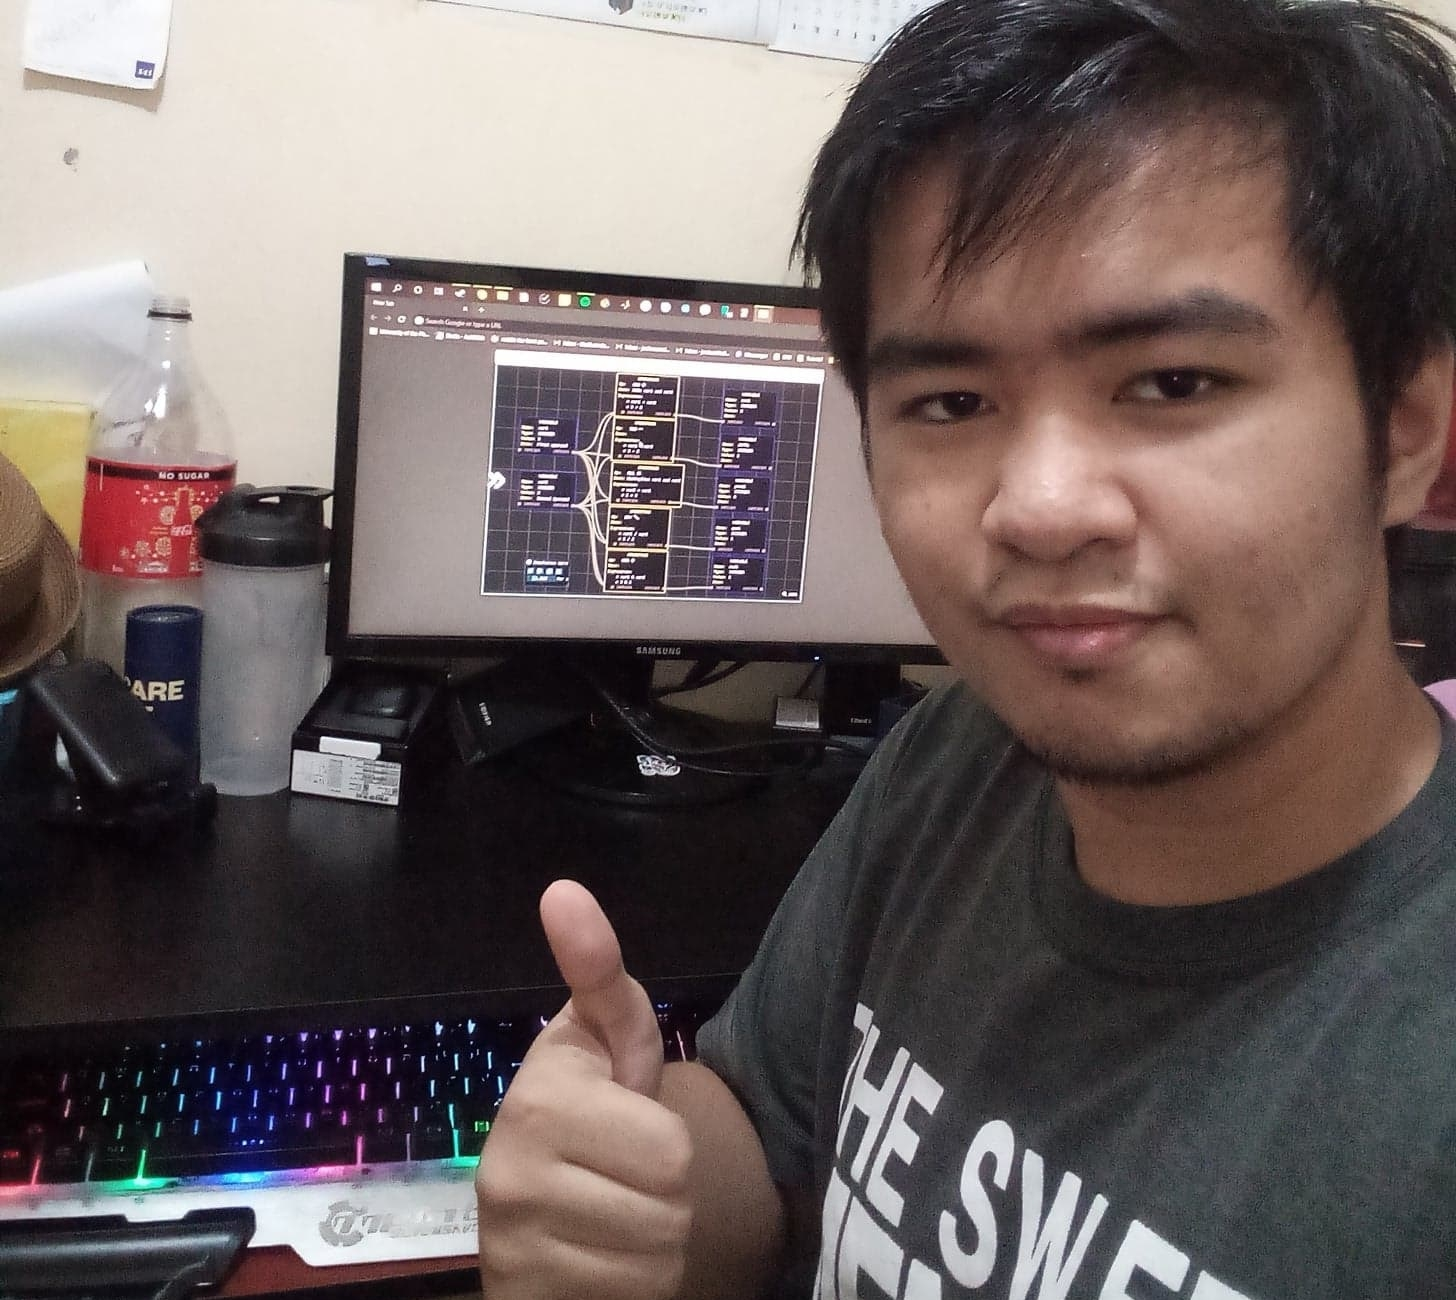
\includegraphics[width=\textwidth]{evaluators/tech/f_rwc.jpg}
\end{figure}
\begin{figure}[H]
	 \centering
	 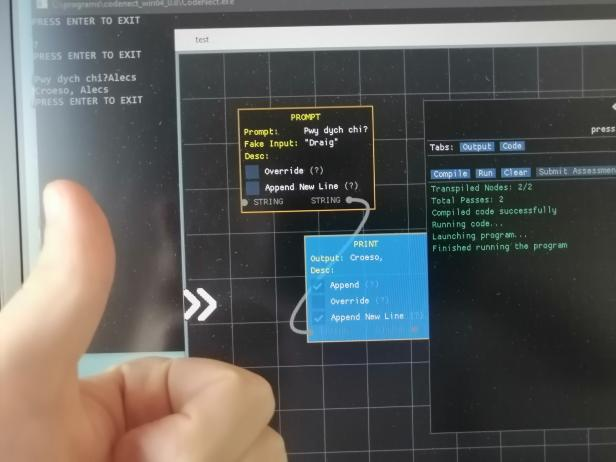
\includegraphics[width=\textwidth]{evaluators/tech/d_a13.jpg}
\end{figure}
\begin{figure}[H]
	 \centering
	 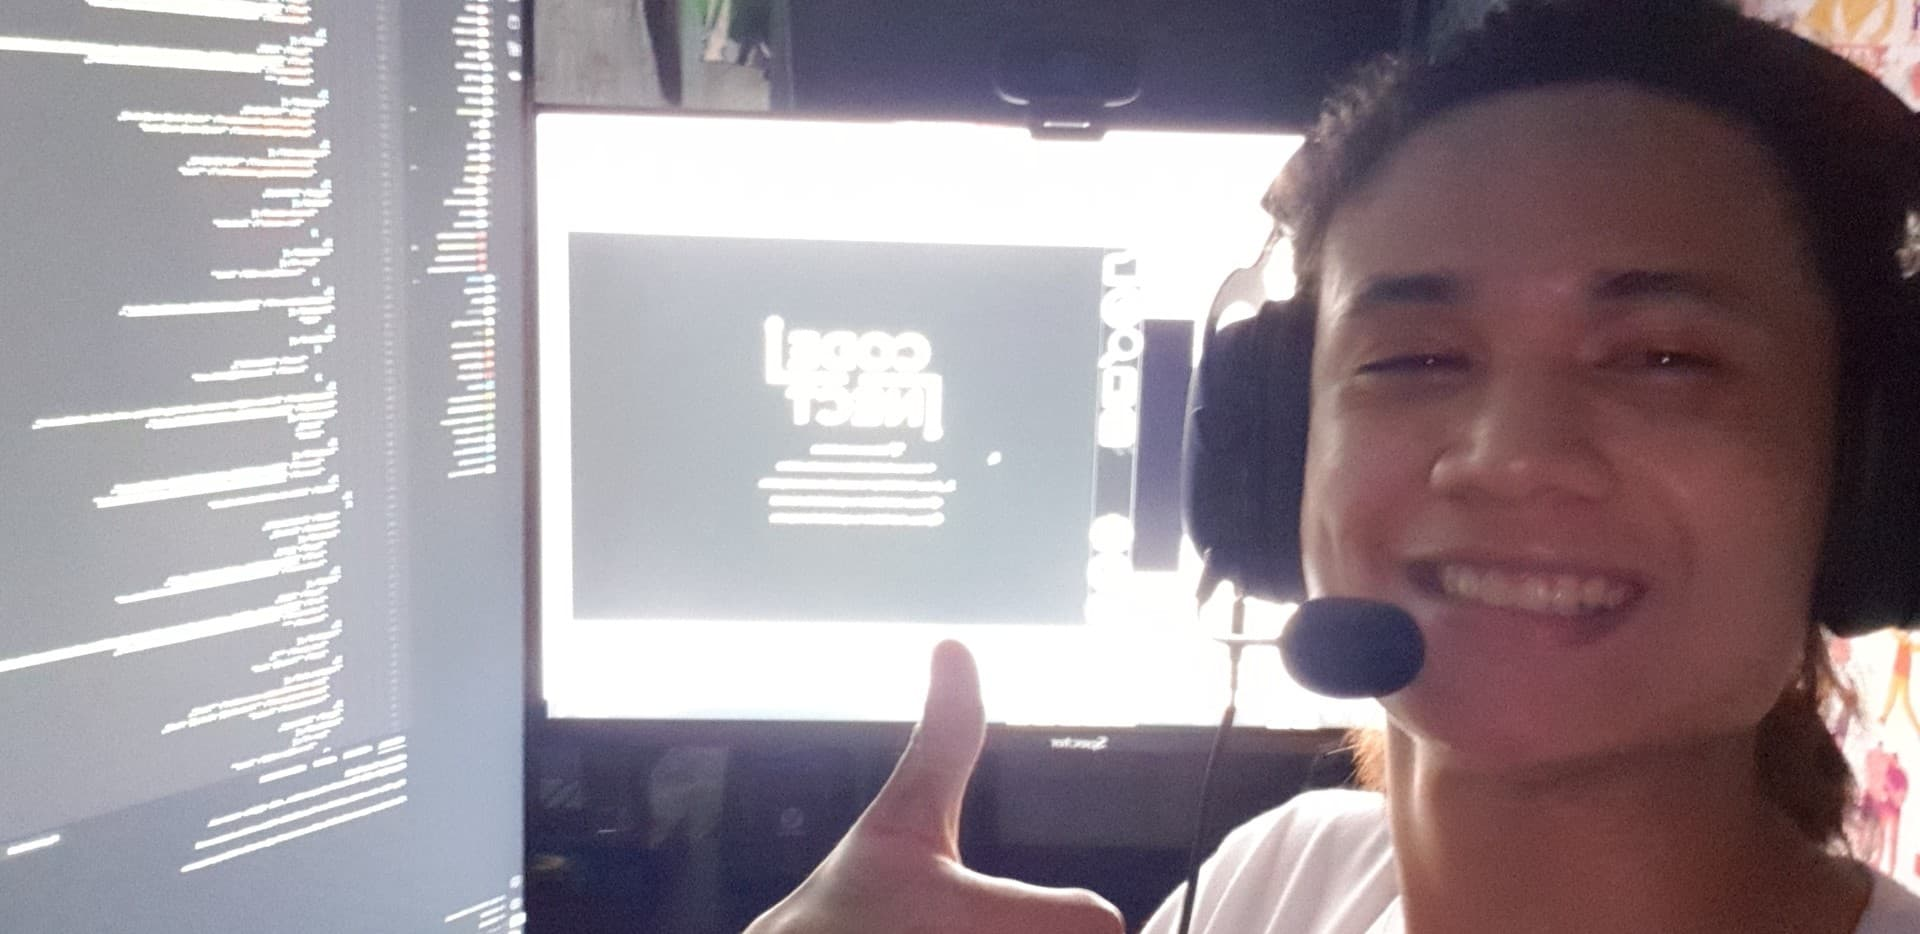
\includegraphics[width=\textwidth]{evaluators/tech/f_un.jpg}
\end{figure}
\begin{figure}[H]
	 \centering
	 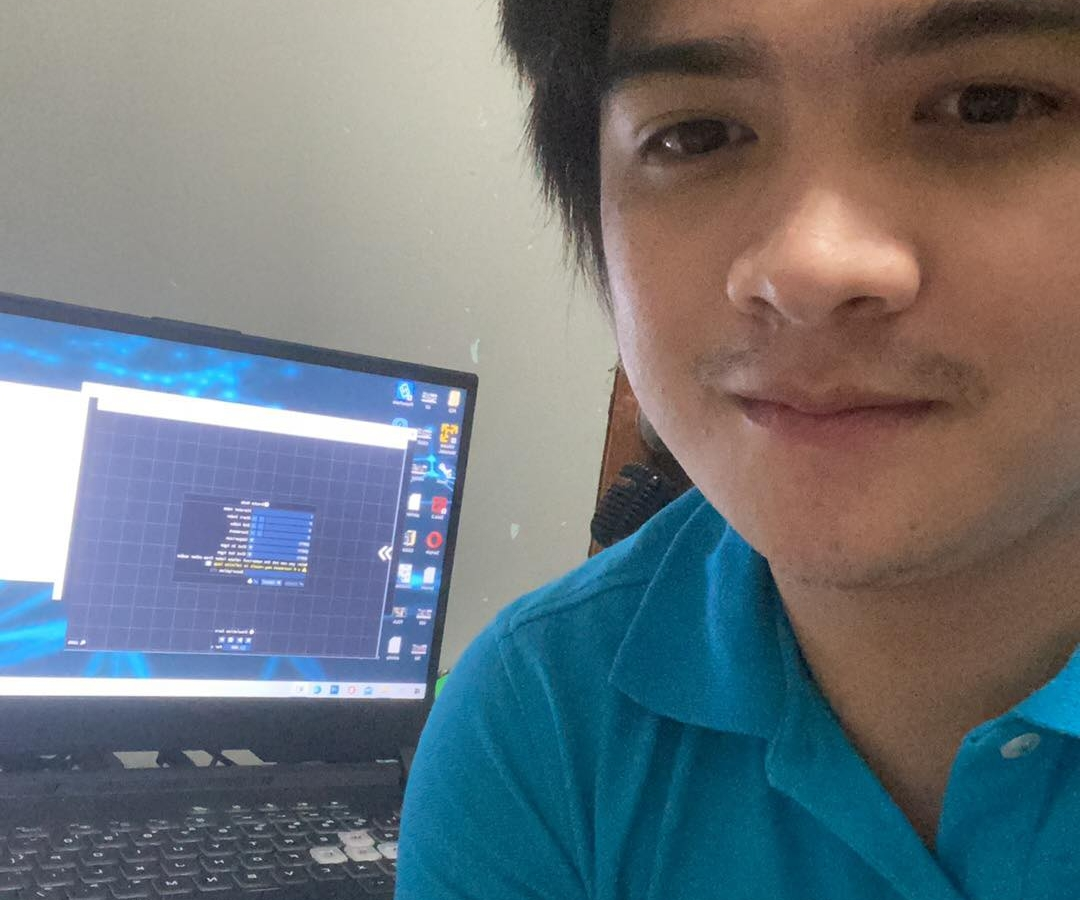
\includegraphics[width=\textwidth]{evaluators/tech/f_un2.jpg}
\end{figure}
\begin{figure}[H]
	 \centering
	 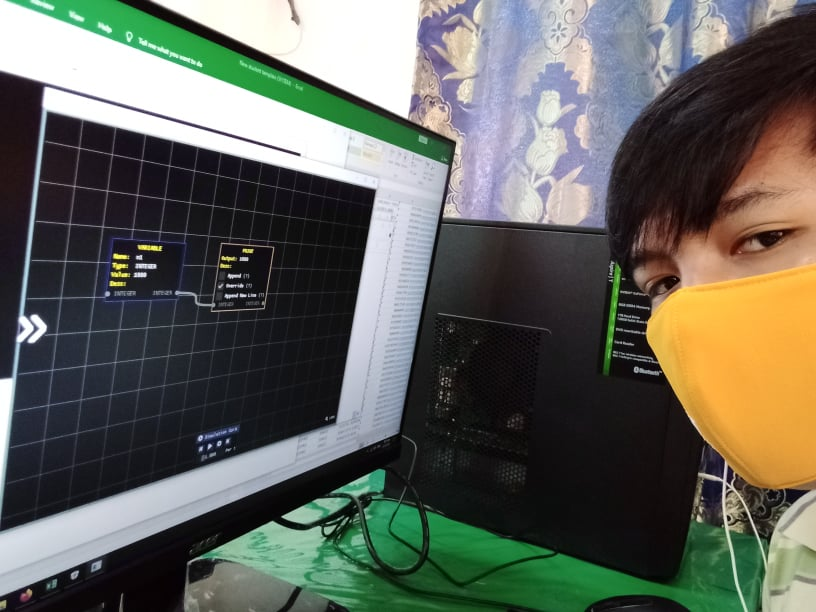
\includegraphics[width=\textwidth]{evaluators/tech/f_ls.jpg}
\end{figure}
\begin{figure}[H]
	 \centering
	 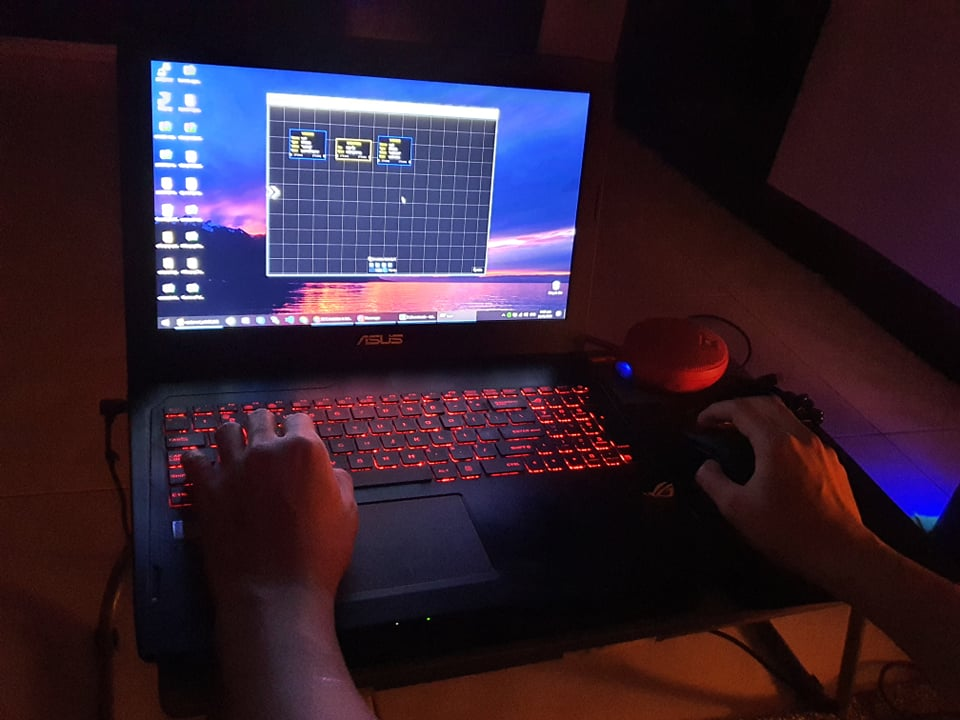
\includegraphics[width=\textwidth]{evaluators/tech/f_jb.jpg}
	 \caption[]{IT/CS Professionals Software Evaluation Pictures}
\end{figure}

% NON-TECH EVALUATORS
\clearpage
\begin{figure}[H]
	 \centering
	 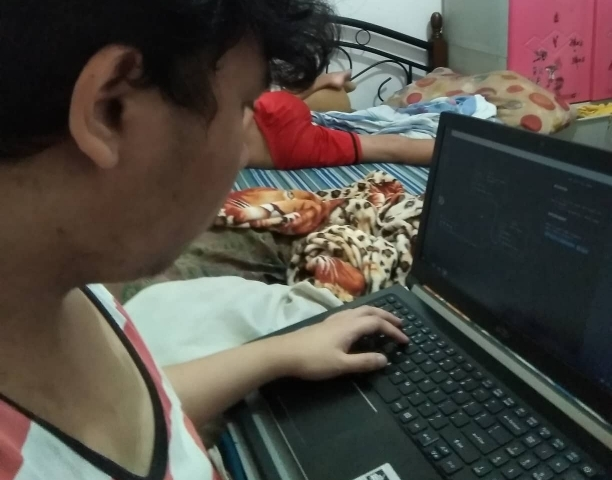
\includegraphics[width=\textwidth]{evaluators/non_tech/f_ec.jpg}
\end{figure}
\begin{figure}[H]
	 \centering
	 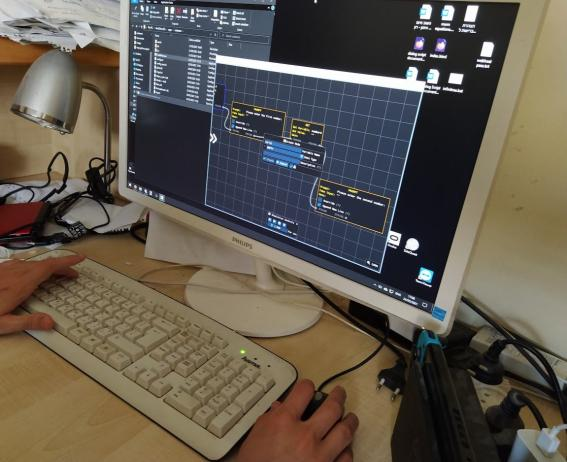
\includegraphics[width=\textwidth]{evaluators/non_tech/d_sr.jpg}
\end{figure}
\begin{figure}[H]
	 \centering
	 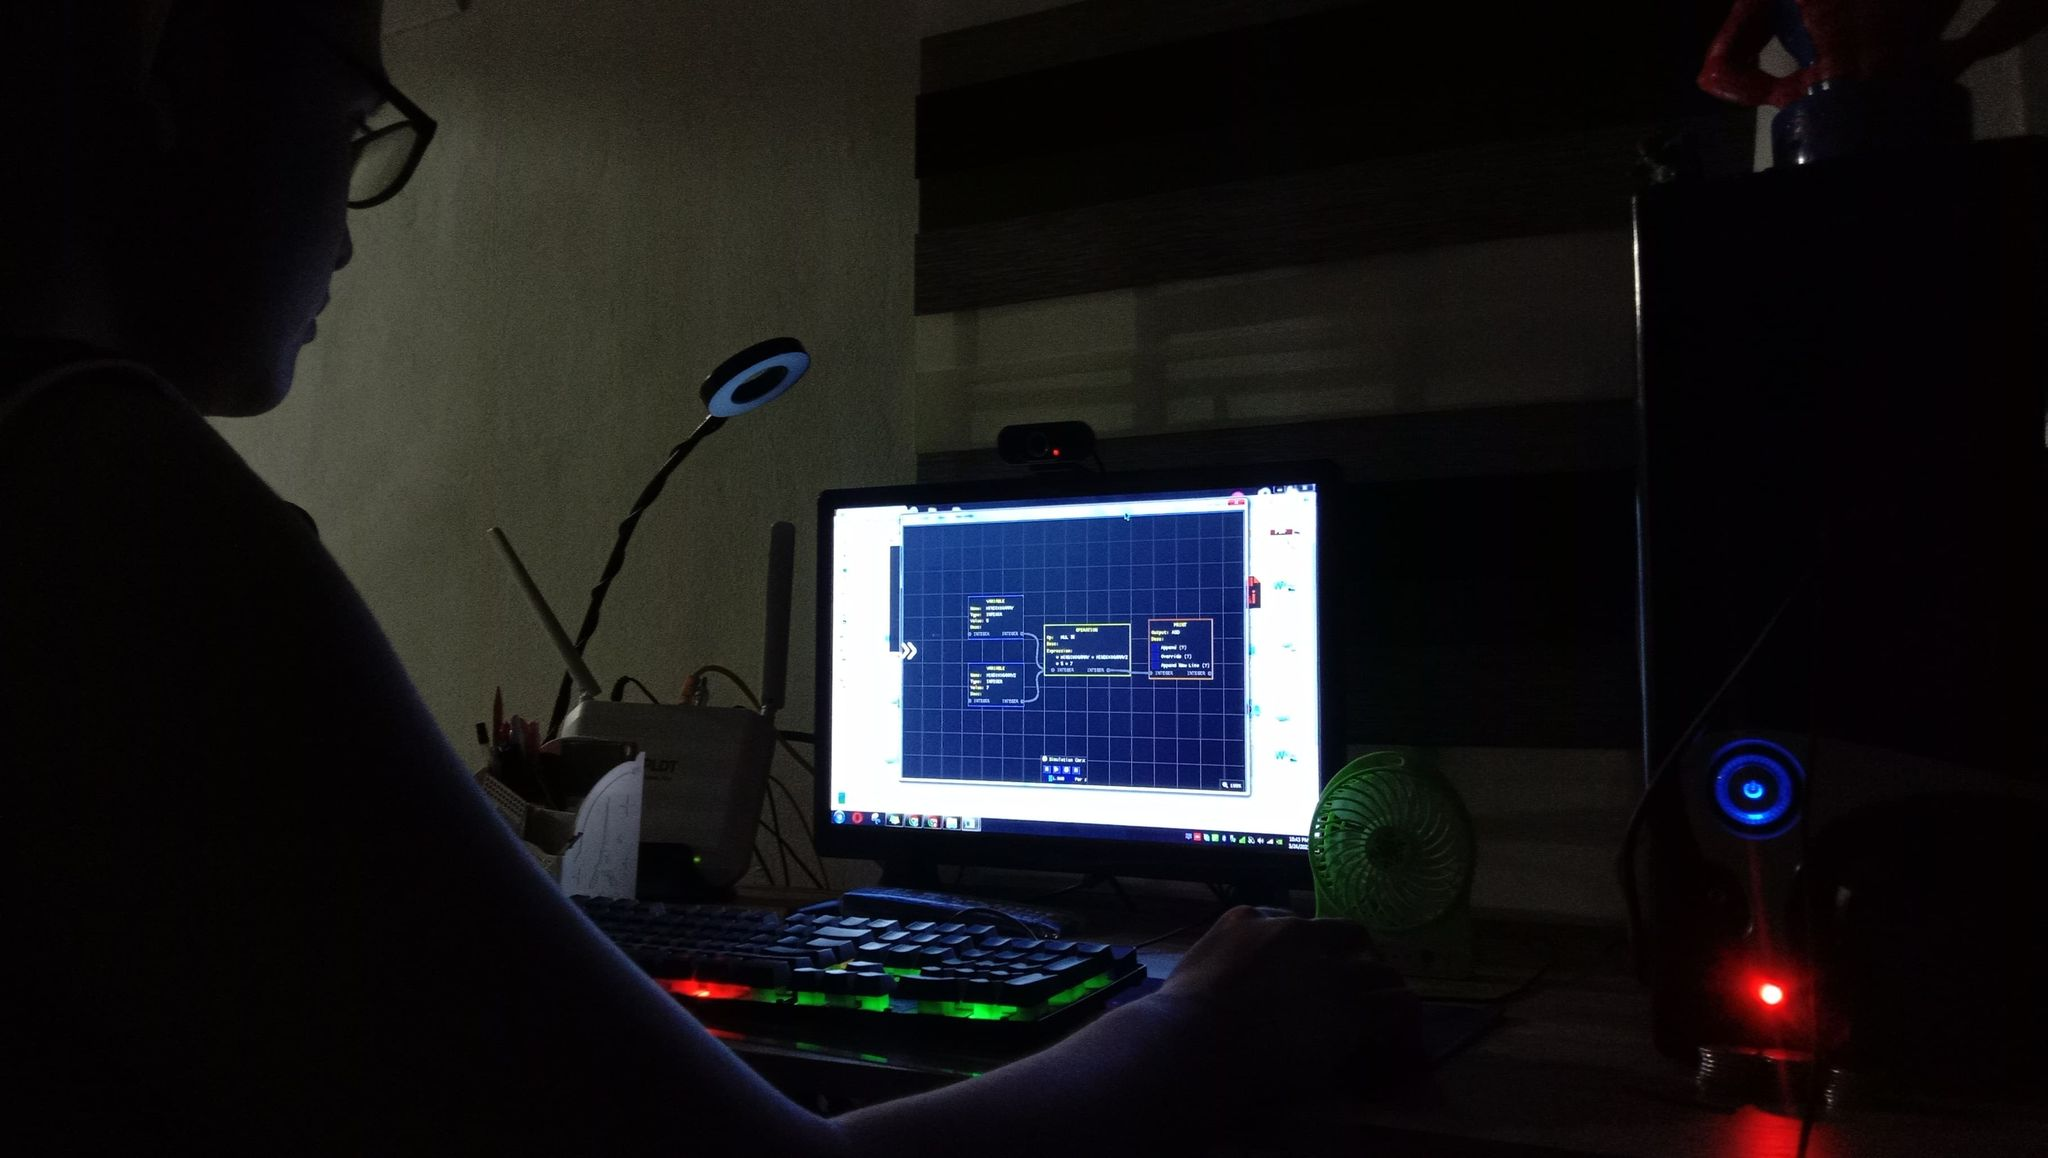
\includegraphics[width=\textwidth]{evaluators/non_tech/f_am.jpg}
\end{figure}
\begin{figure}[H]
	 \centering
	 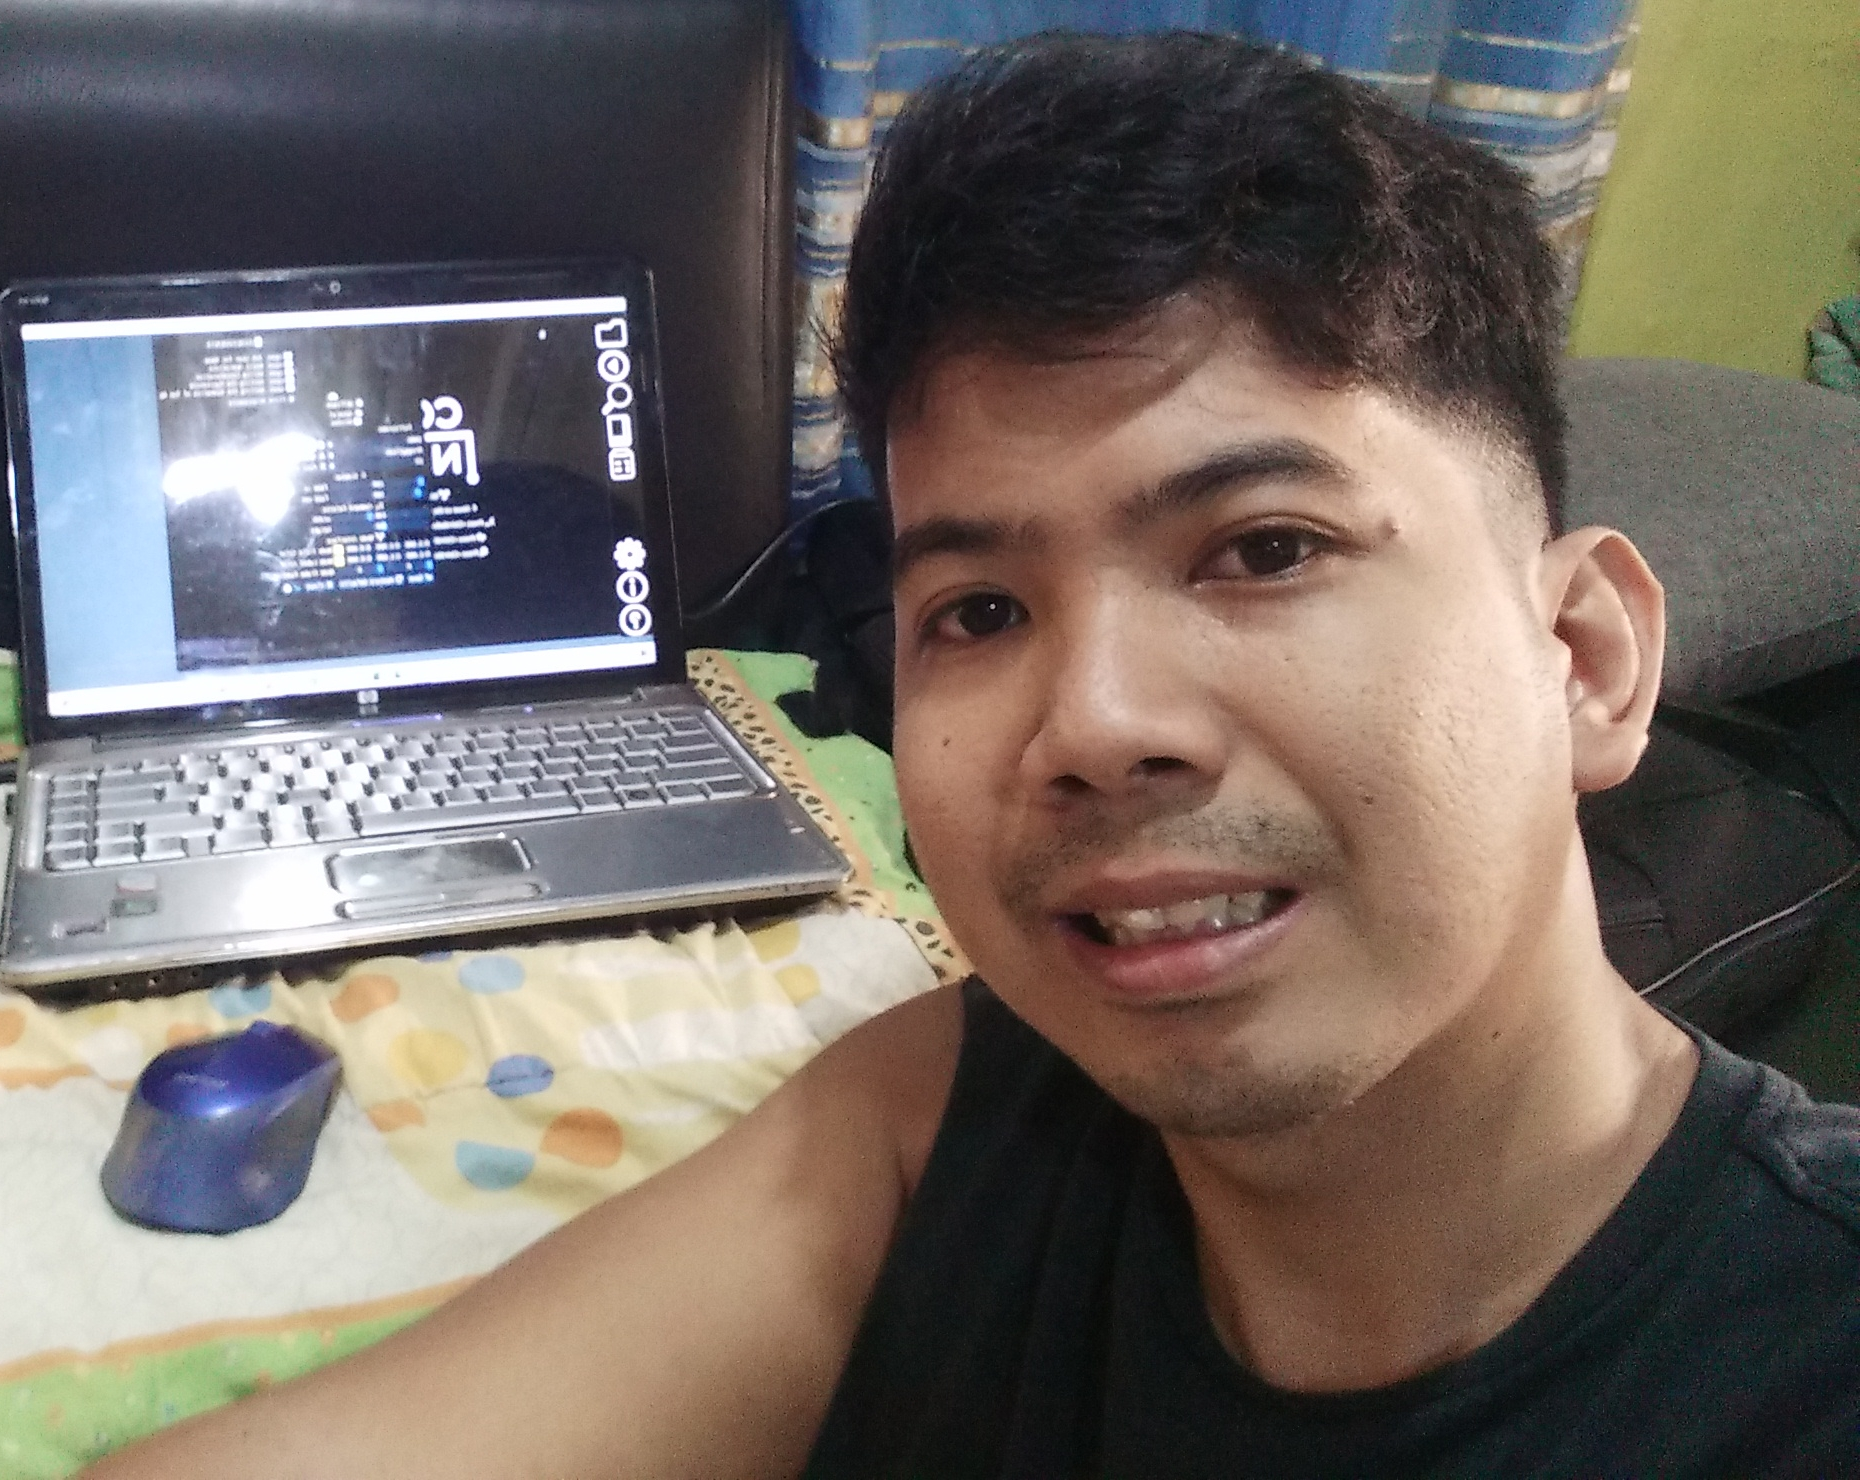
\includegraphics[width=\textwidth]{evaluators/non_tech/f_mr.jpg}
\end{figure}
\begin{figure}[H]
	 \centering
	 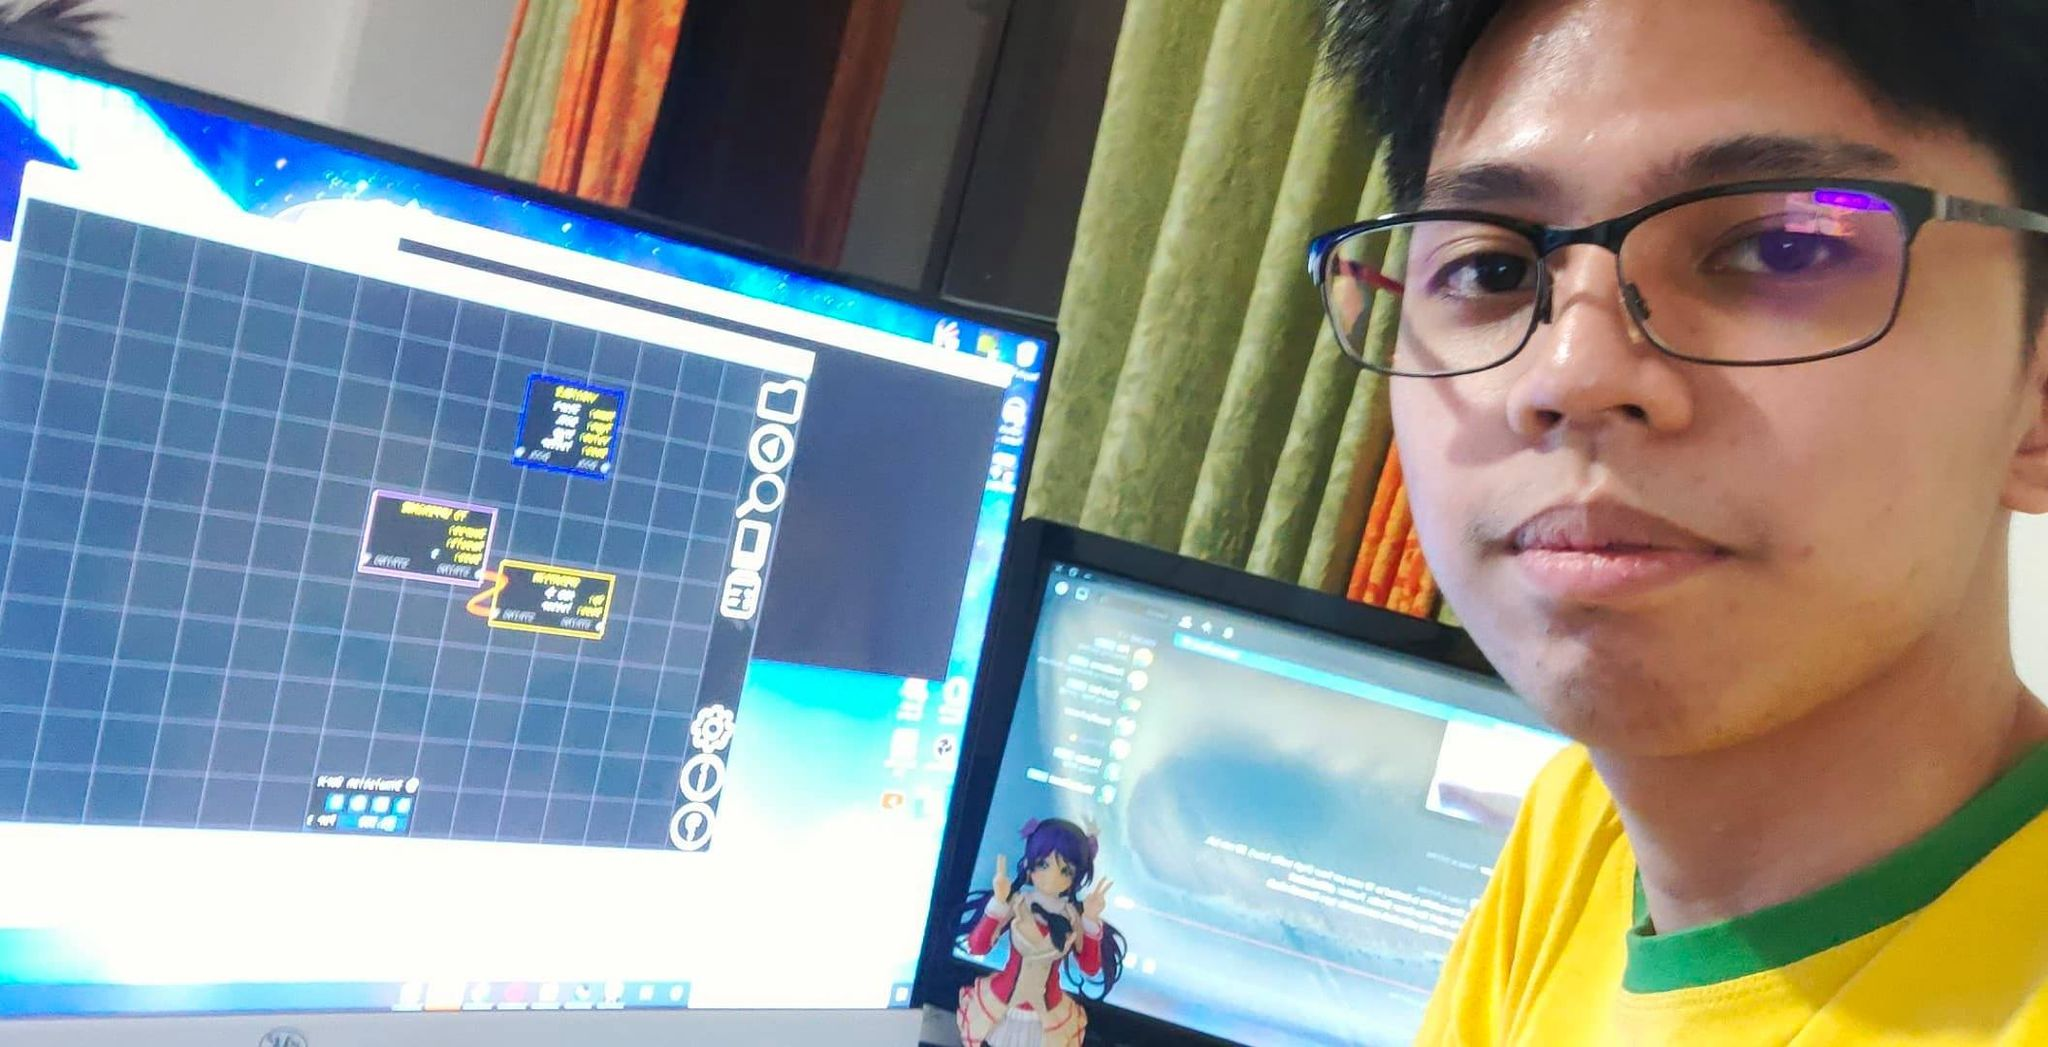
\includegraphics[width=\textwidth]{evaluators/non_tech/f_ip.jpg}
	 \caption[]{IT/CS Students Software Evaluation Pictures}
\end{figure}

		\clearpage
\app{Relevant Source Code}

\begin{figure}[H]
	 \centering
	 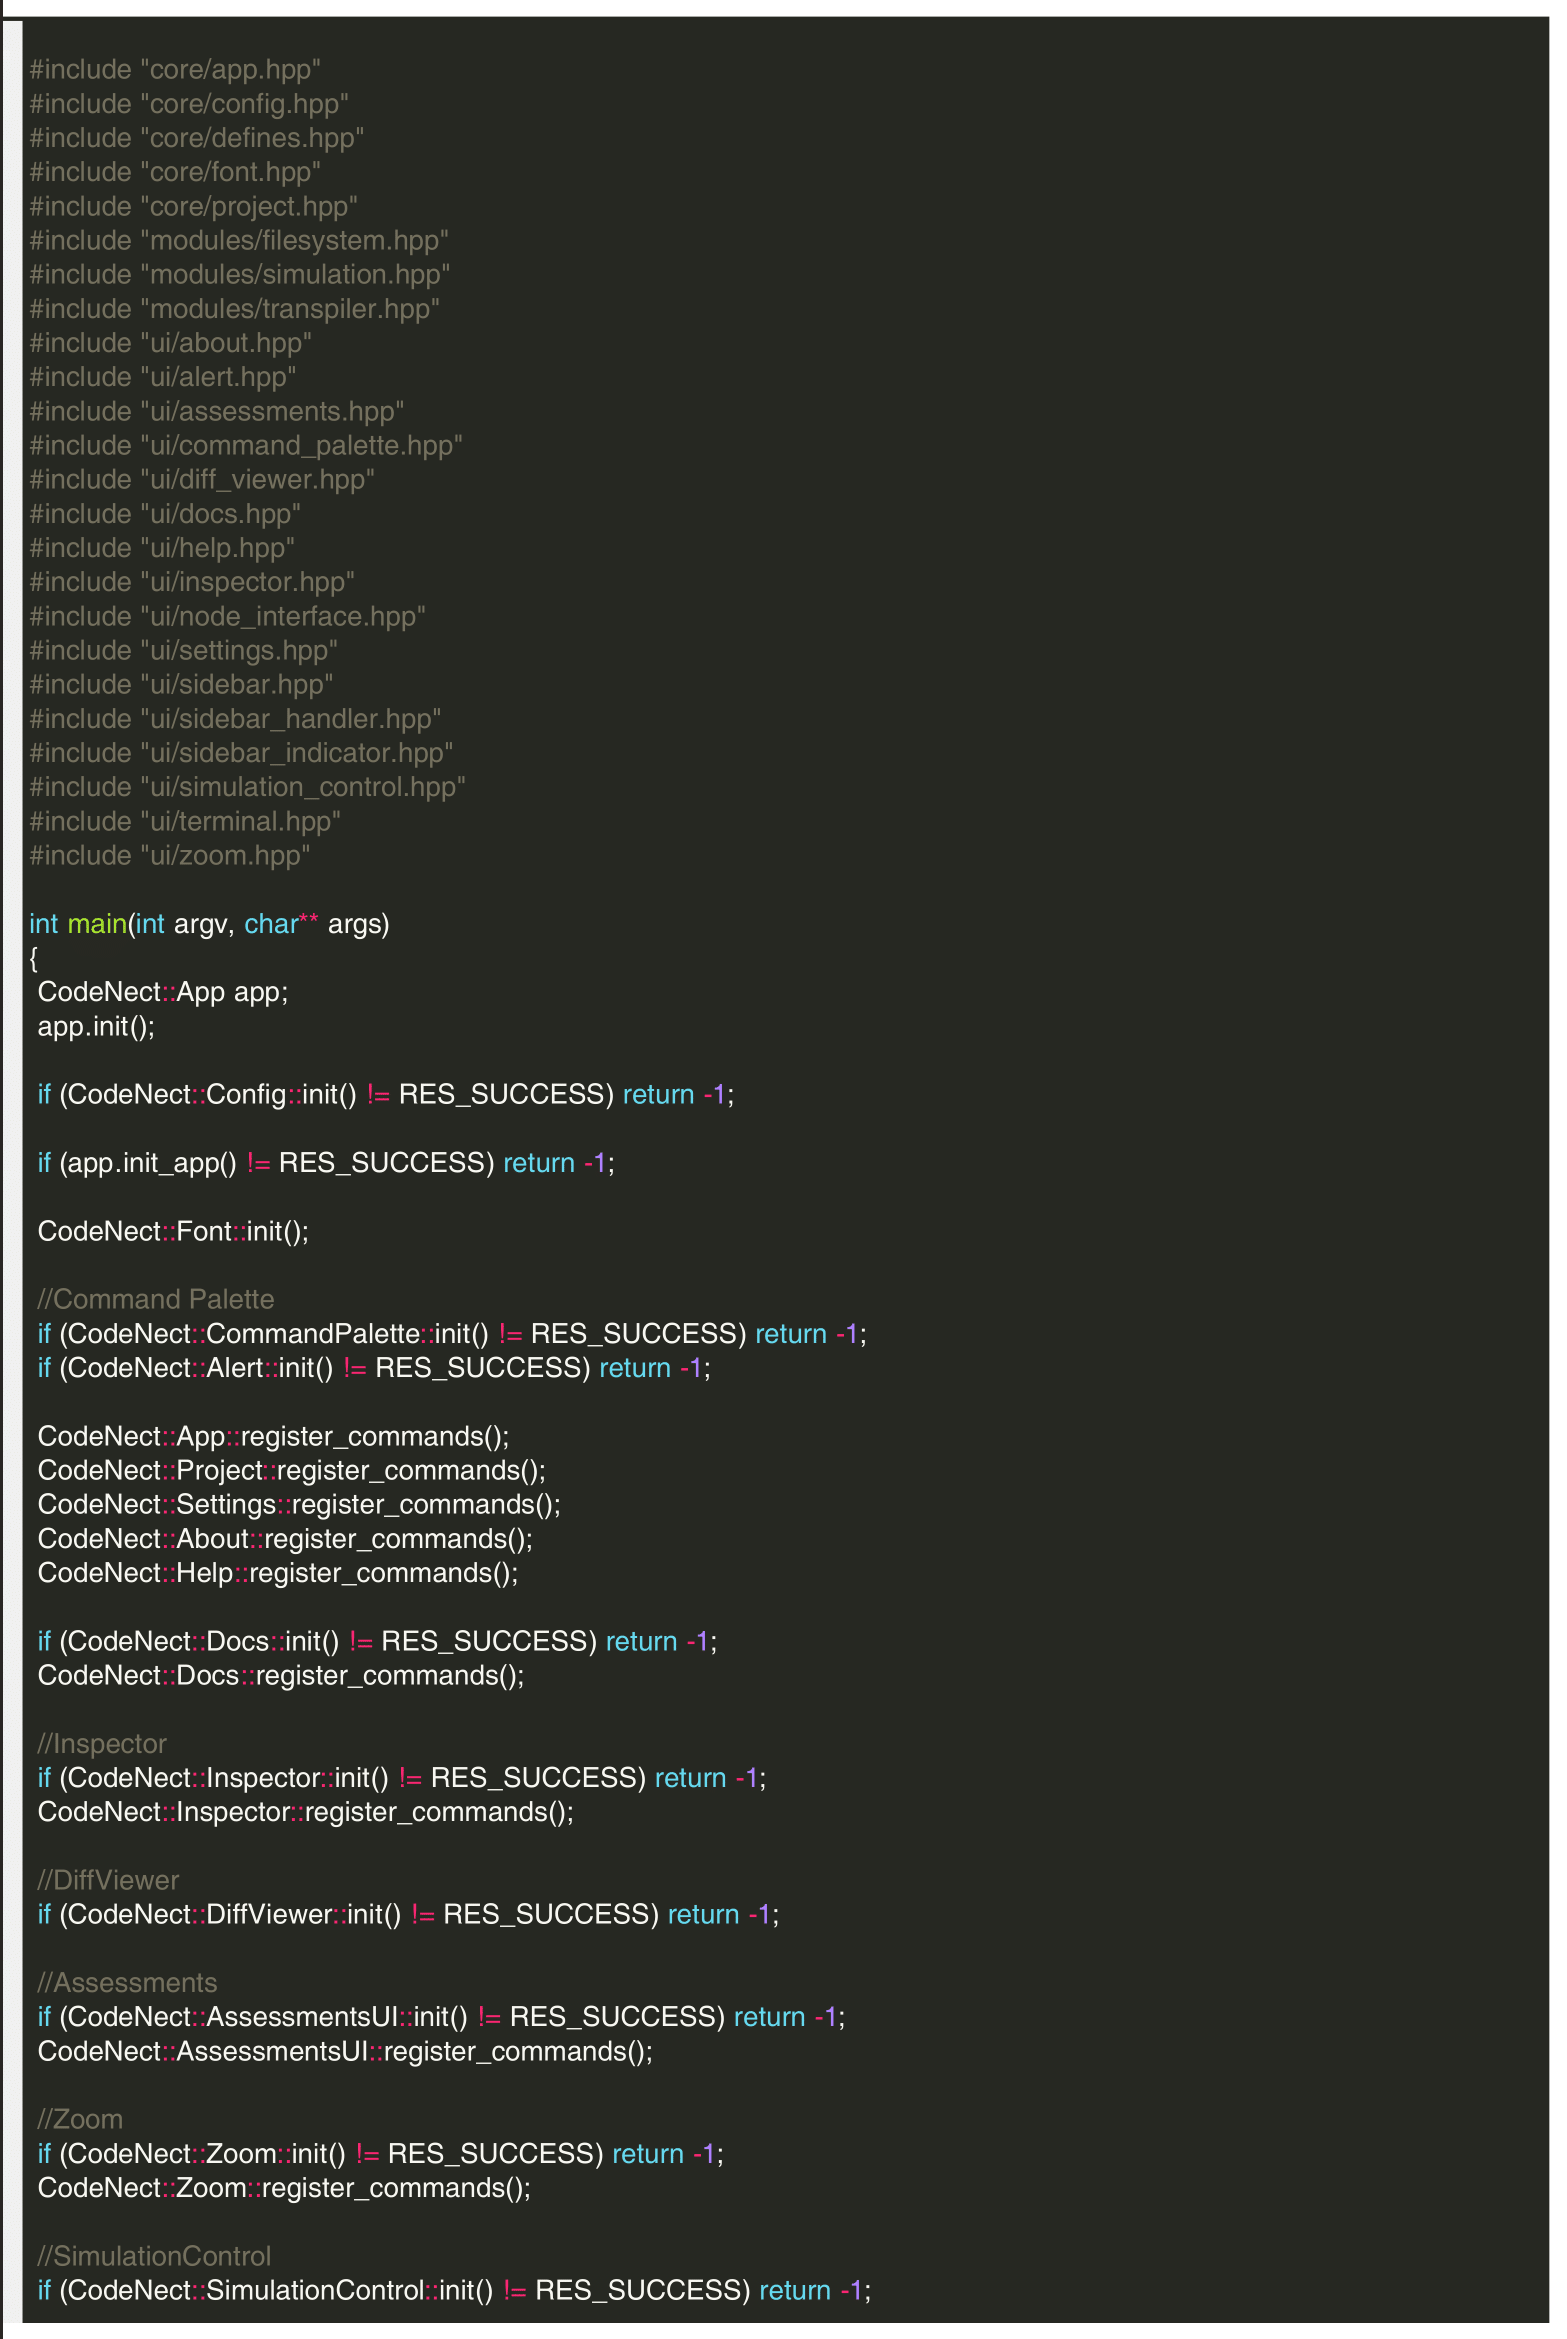
\includegraphics[width=\textwidth]{figures/code/main-1.png}
\end{figure}
\begin{figure}[H]
	 \centering
	 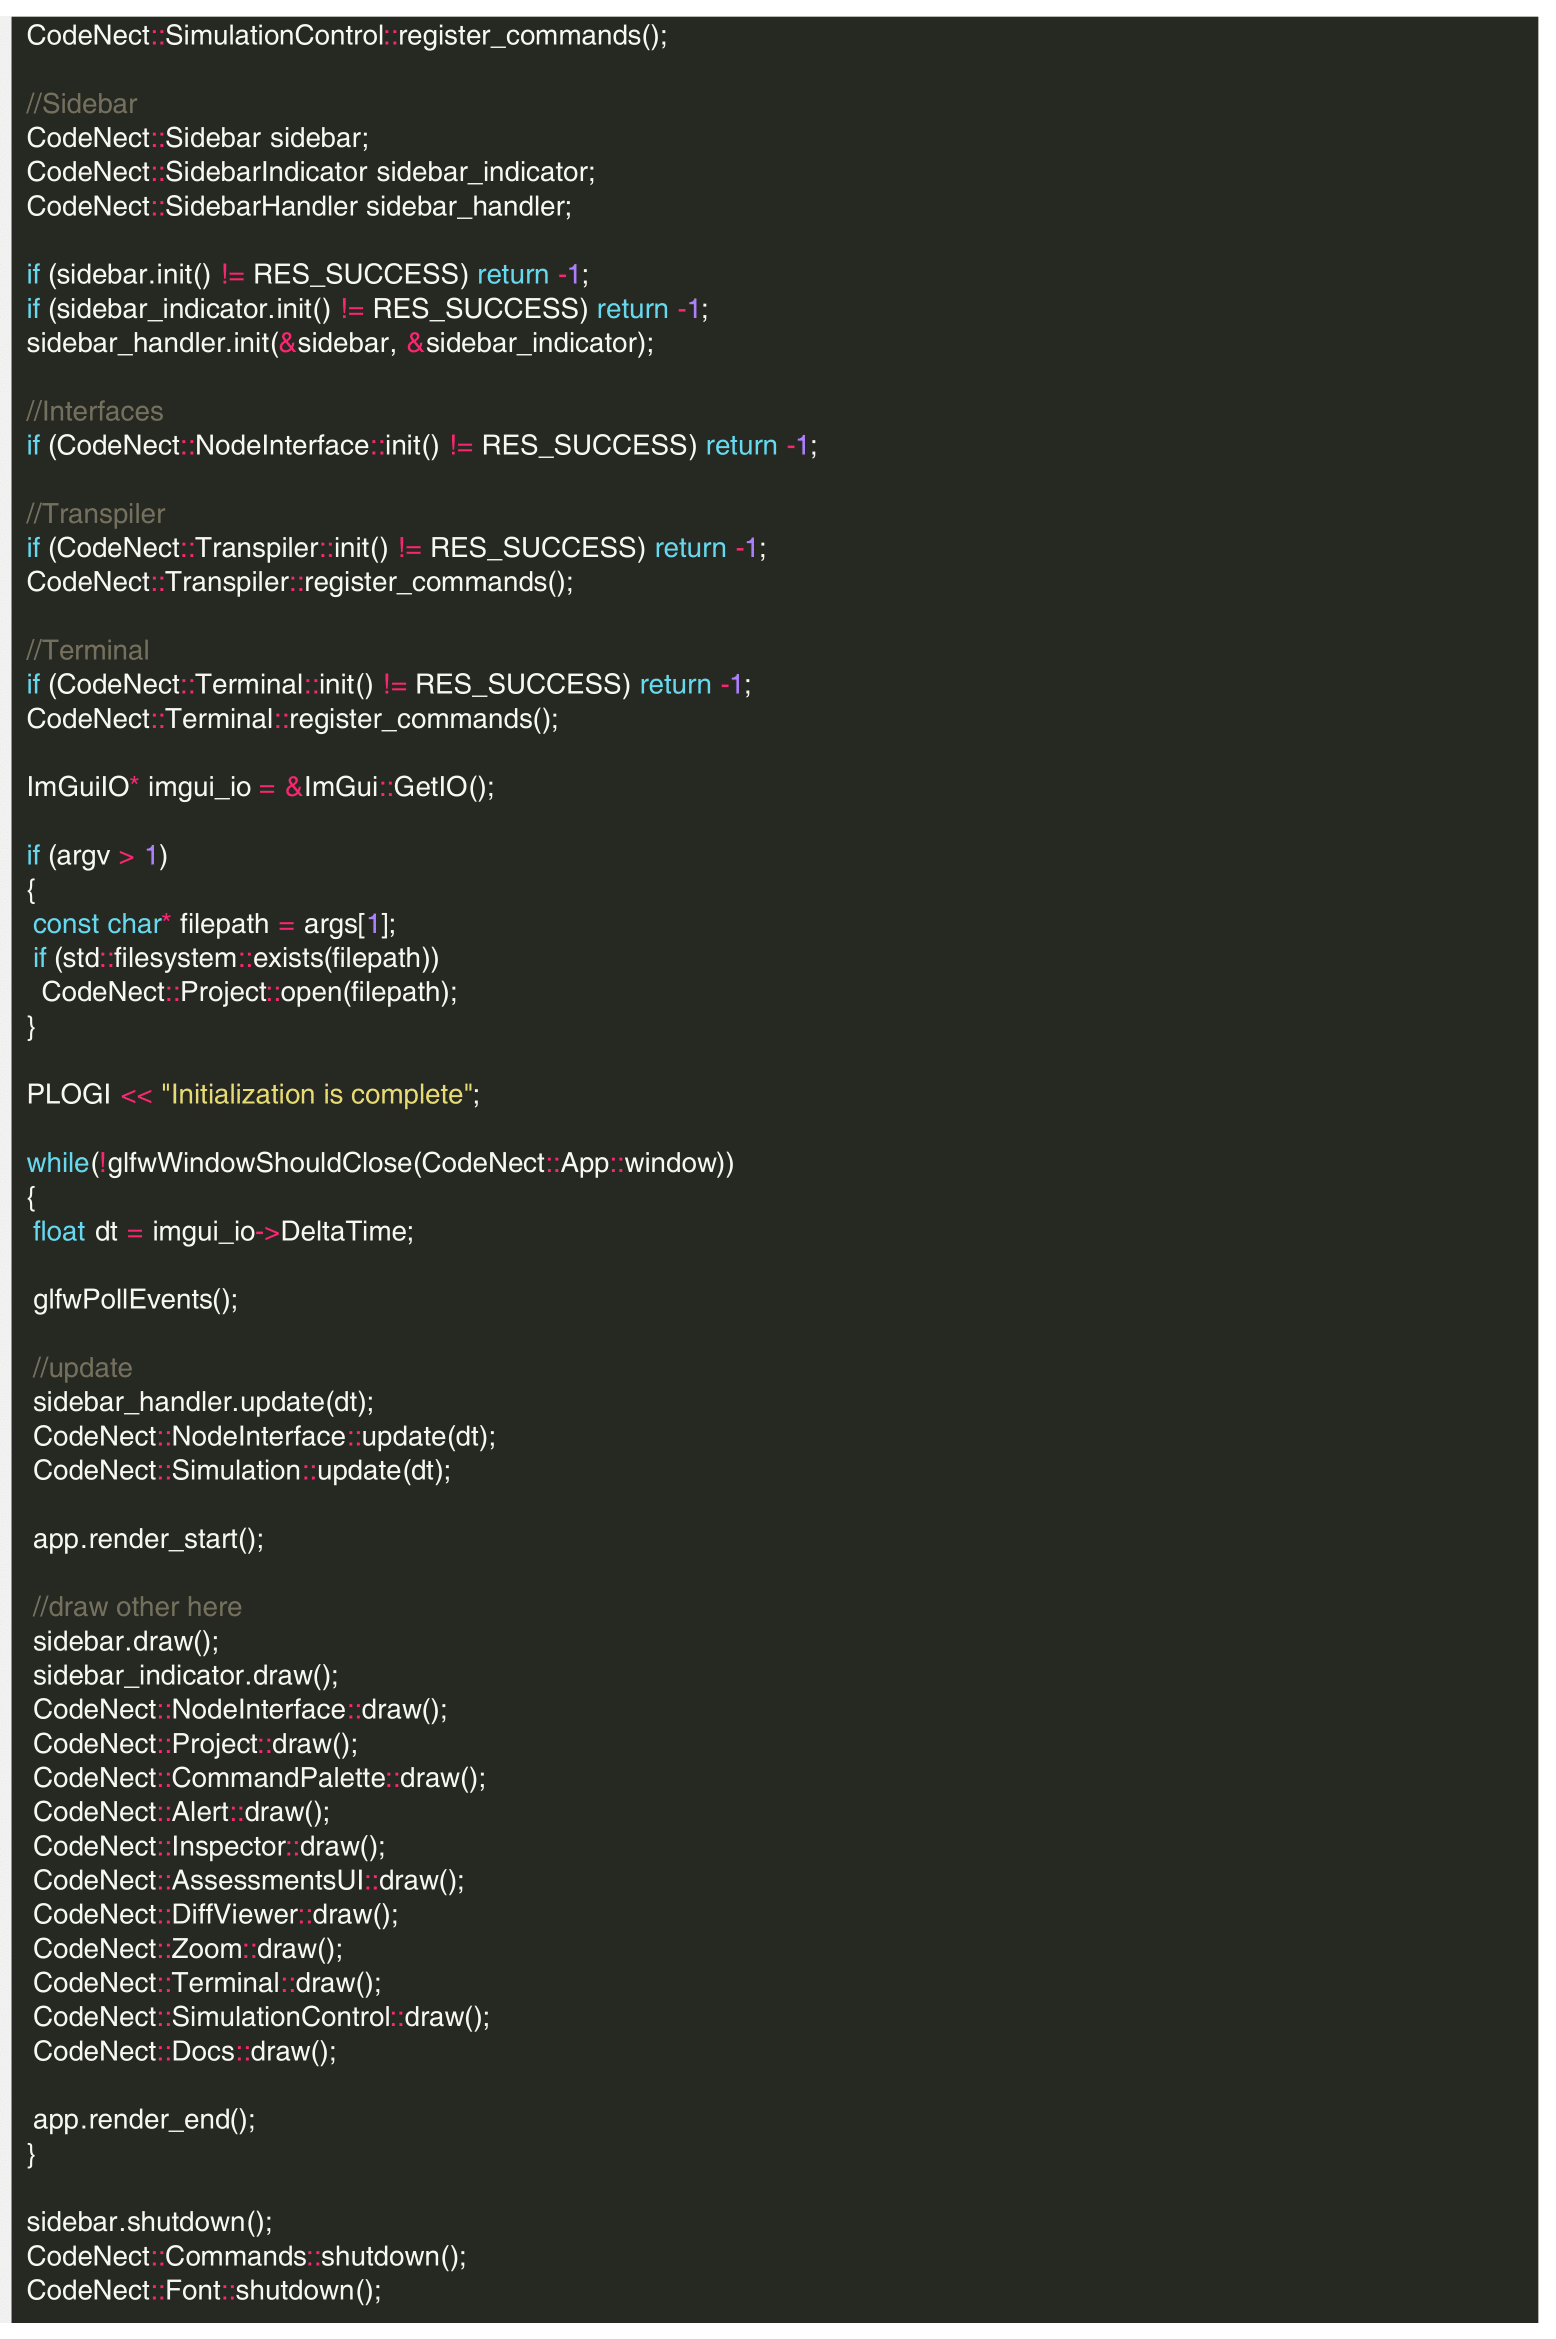
\includegraphics[width=\textwidth]{figures/code/main-2.png}
\end{figure}
\begin{figure}[H]
	 \centering
	 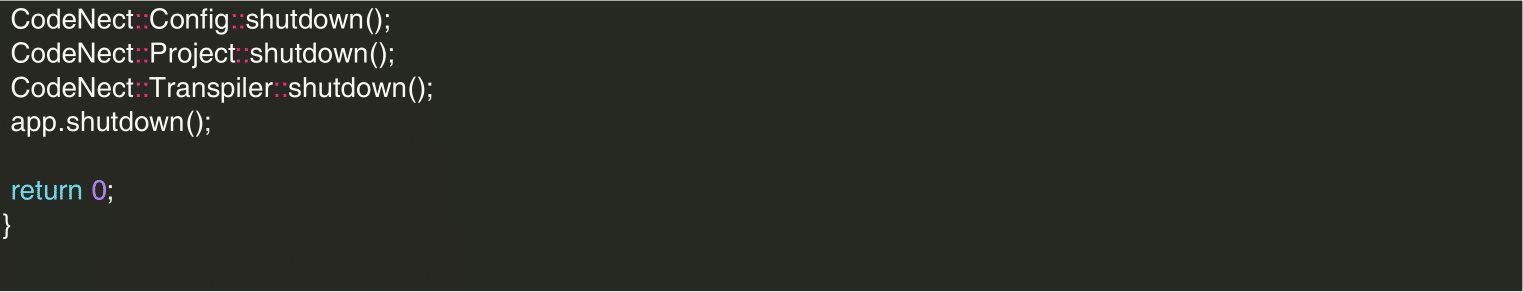
\includegraphics[width=\textwidth]{figures/code/main-3.png}
\end{figure}

\begin{figure}[H]
	 \centering
	 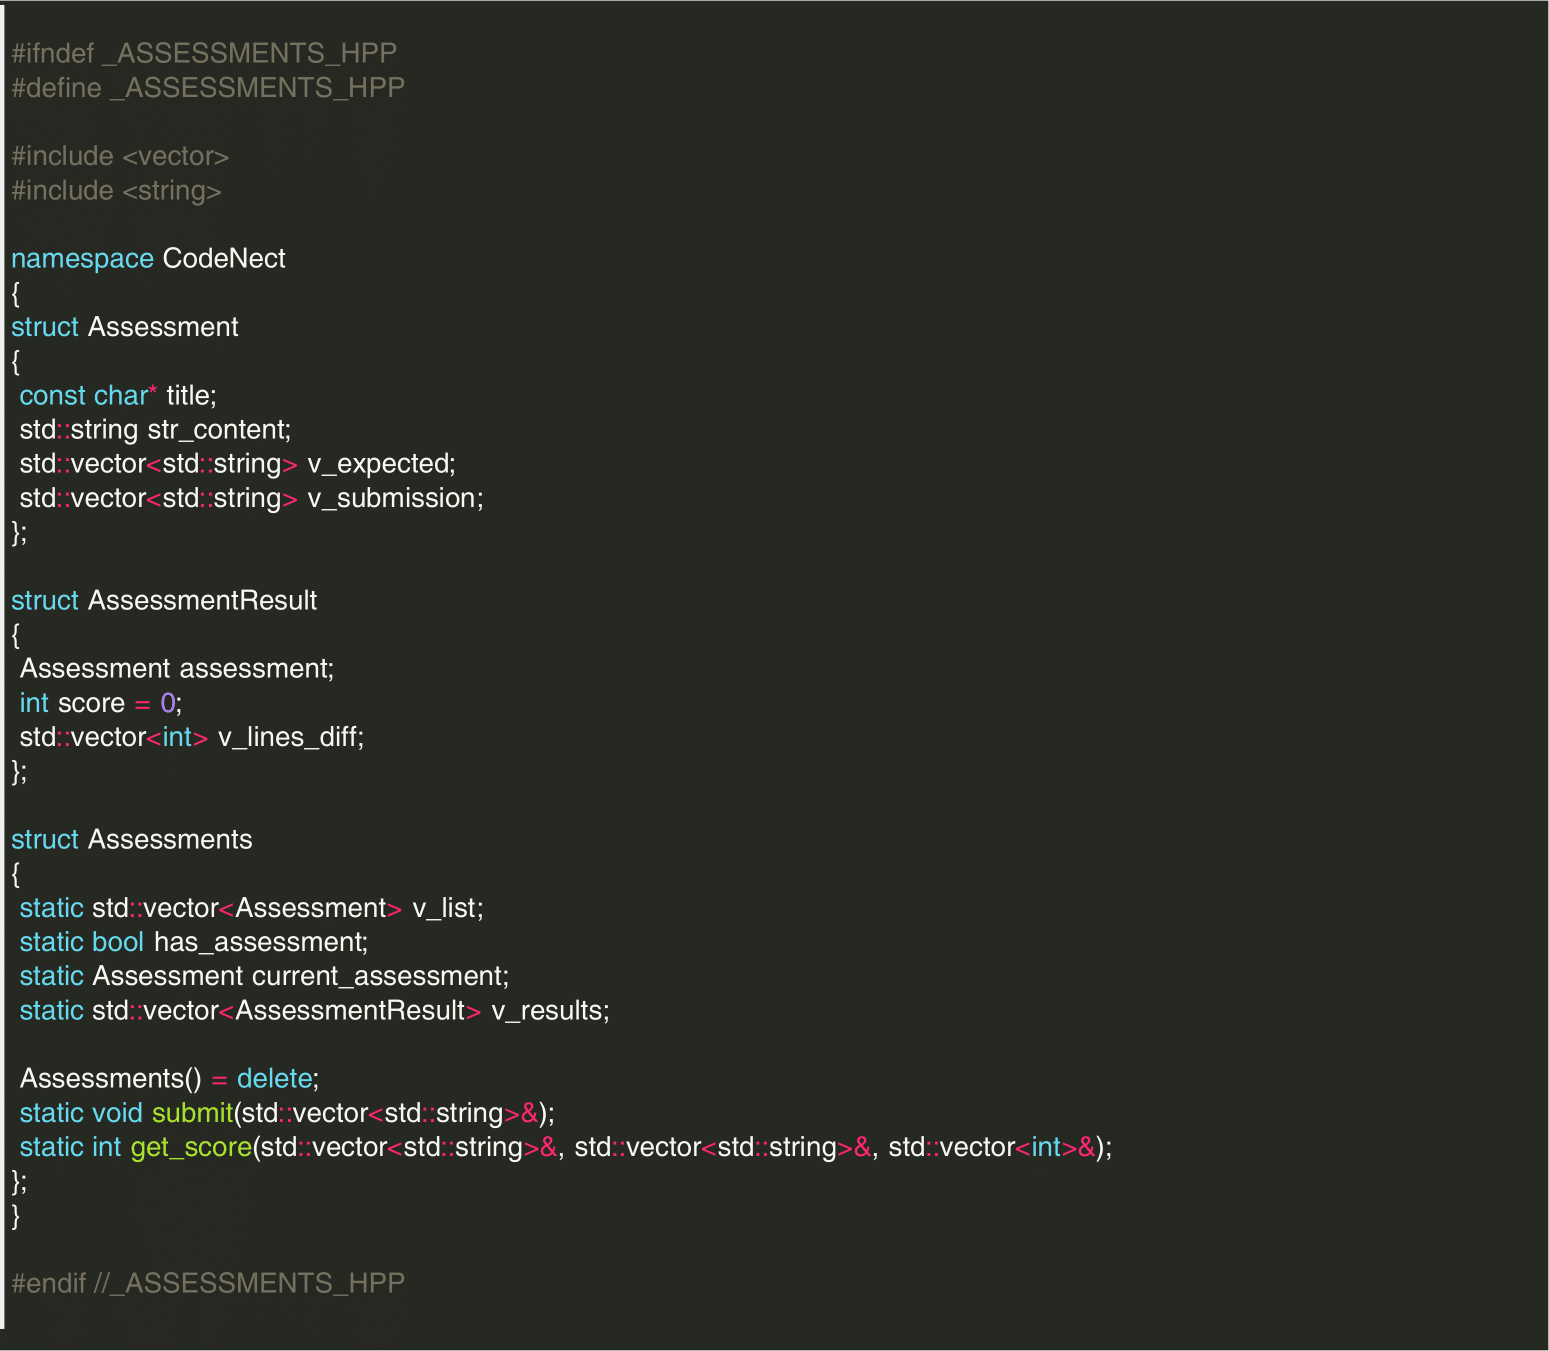
\includegraphics[width=\textwidth]{figures/code/assessments.png}
\end{figure}
\begin{figure}[H]
	 \centering
	 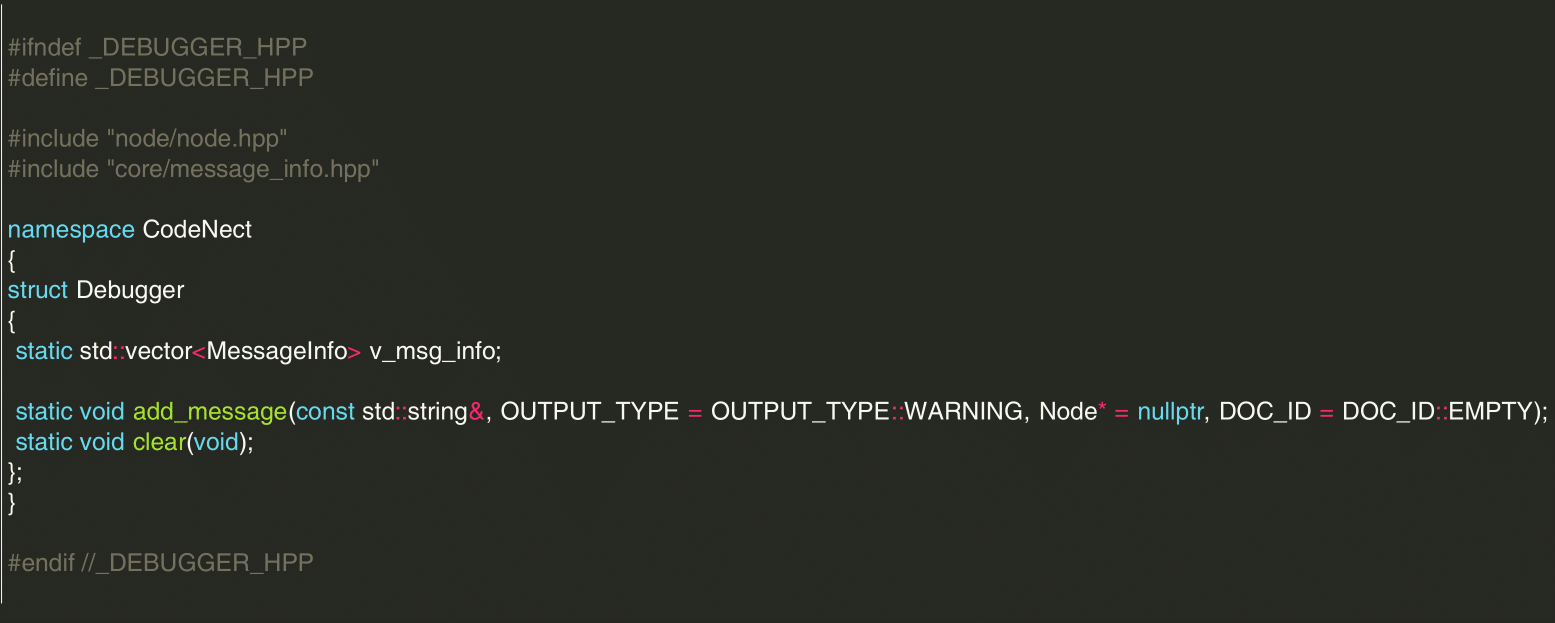
\includegraphics[width=\textwidth]{figures/code/debugger.png}
\end{figure}
\begin{figure}[H]
	 \centering
	 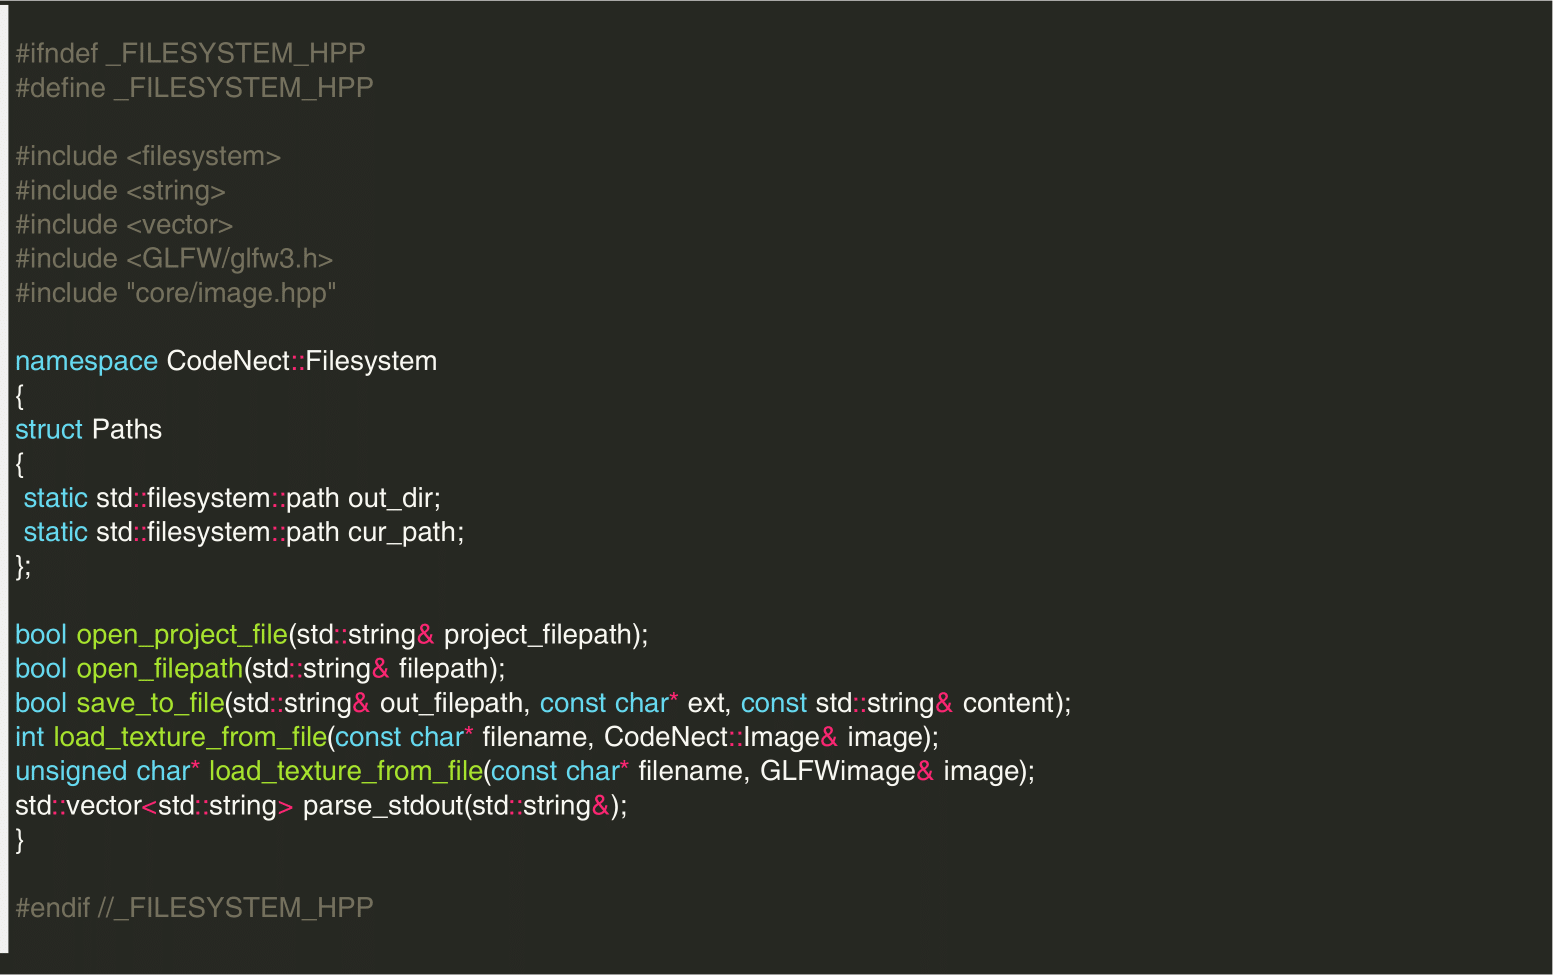
\includegraphics[width=\textwidth]{figures/code/filesystem.png}
\end{figure}
\begin{figure}[H]
	 \centering
	 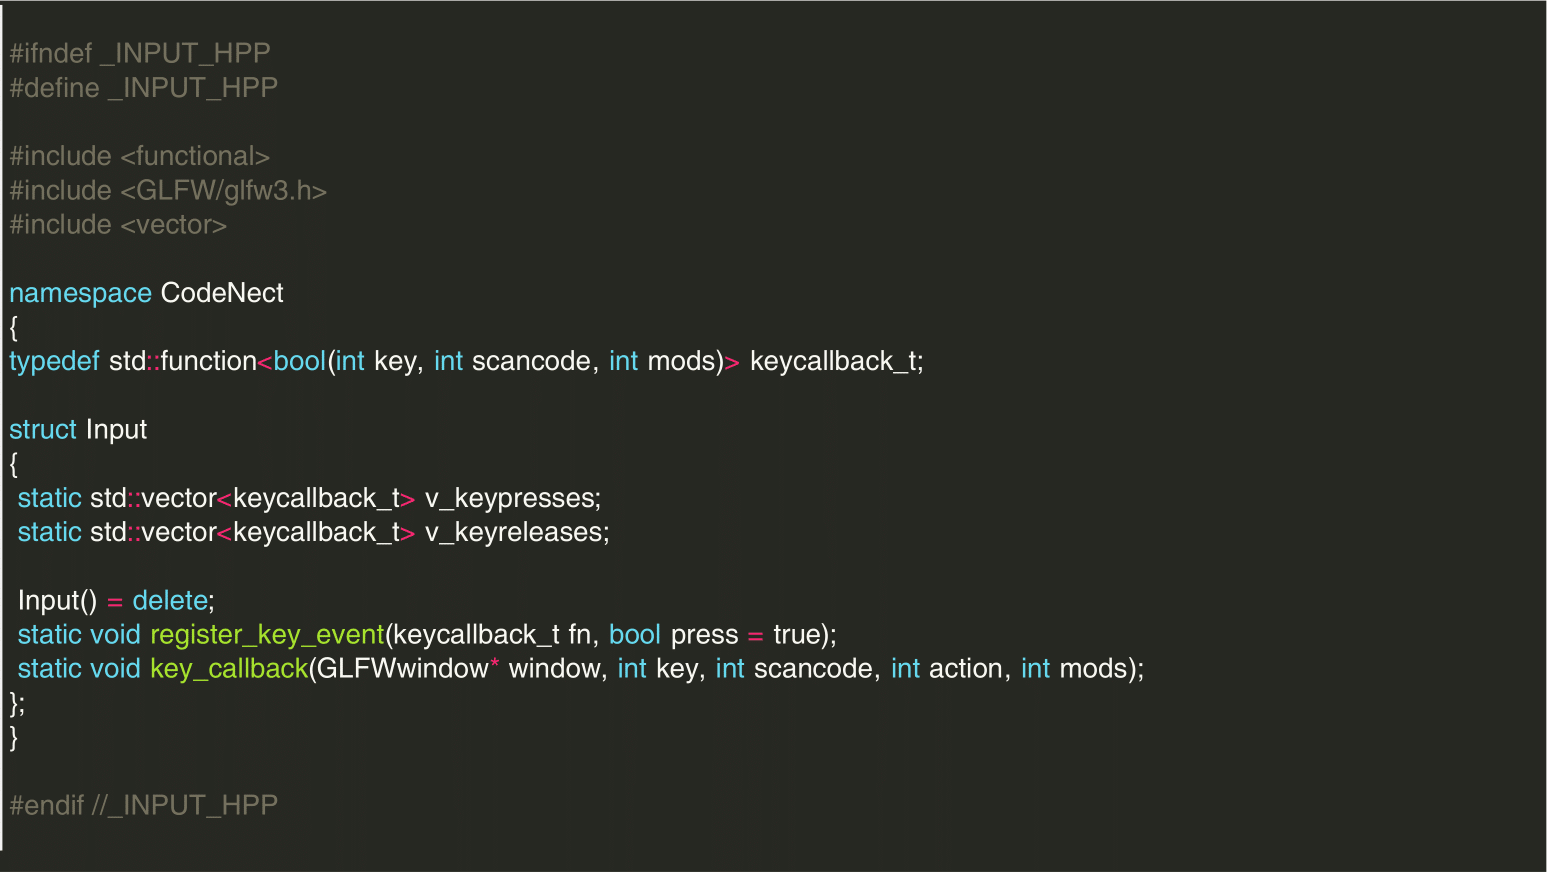
\includegraphics[width=\textwidth]{figures/code/input.png}
\end{figure}
\begin{figure}[H]
	 \centering
	 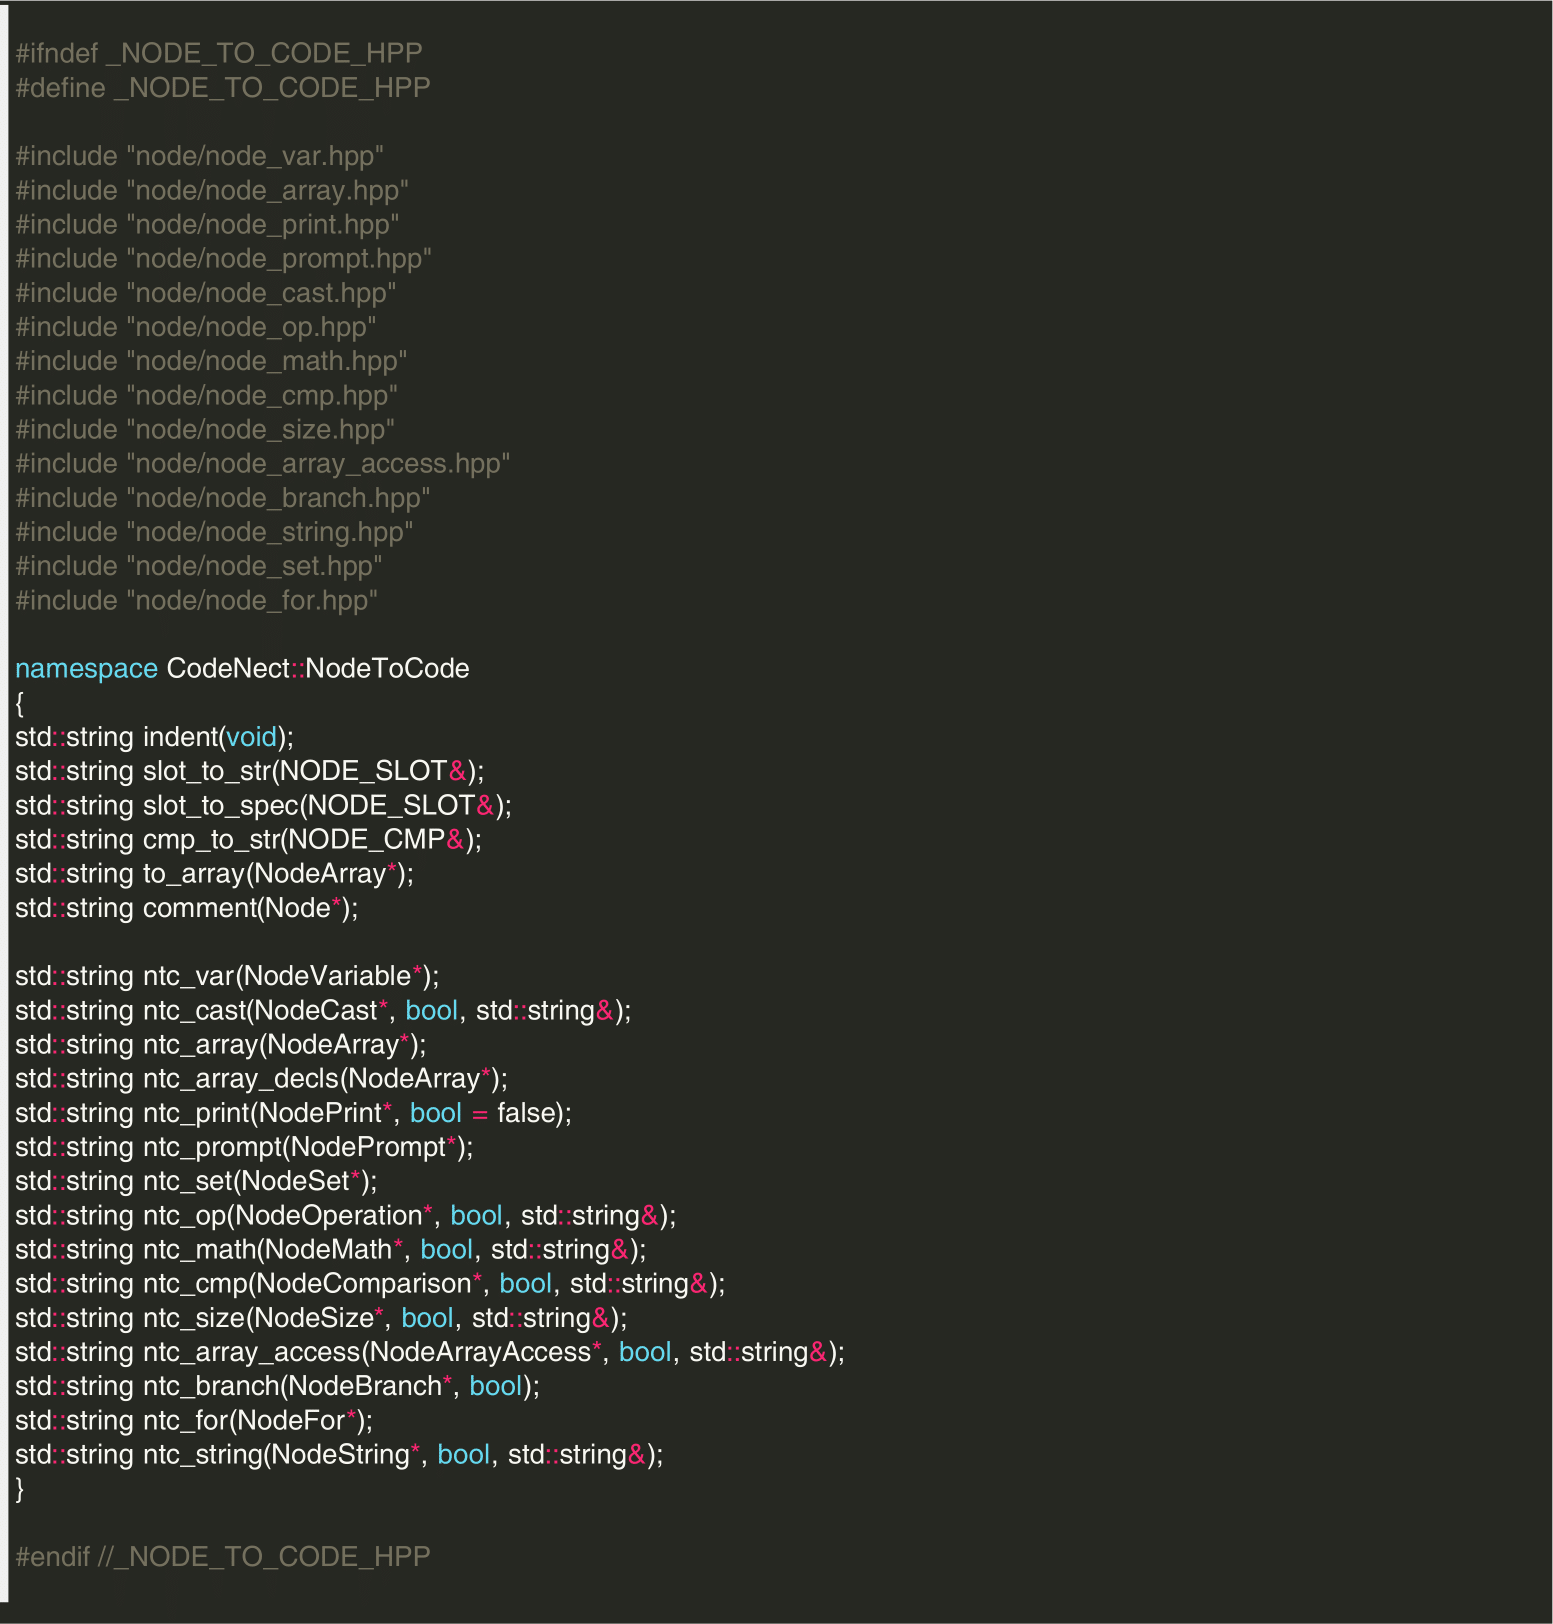
\includegraphics[width=\textwidth]{figures/code/node_to_code.png}
\end{figure}
\begin{figure}[H]
	 \centering
	 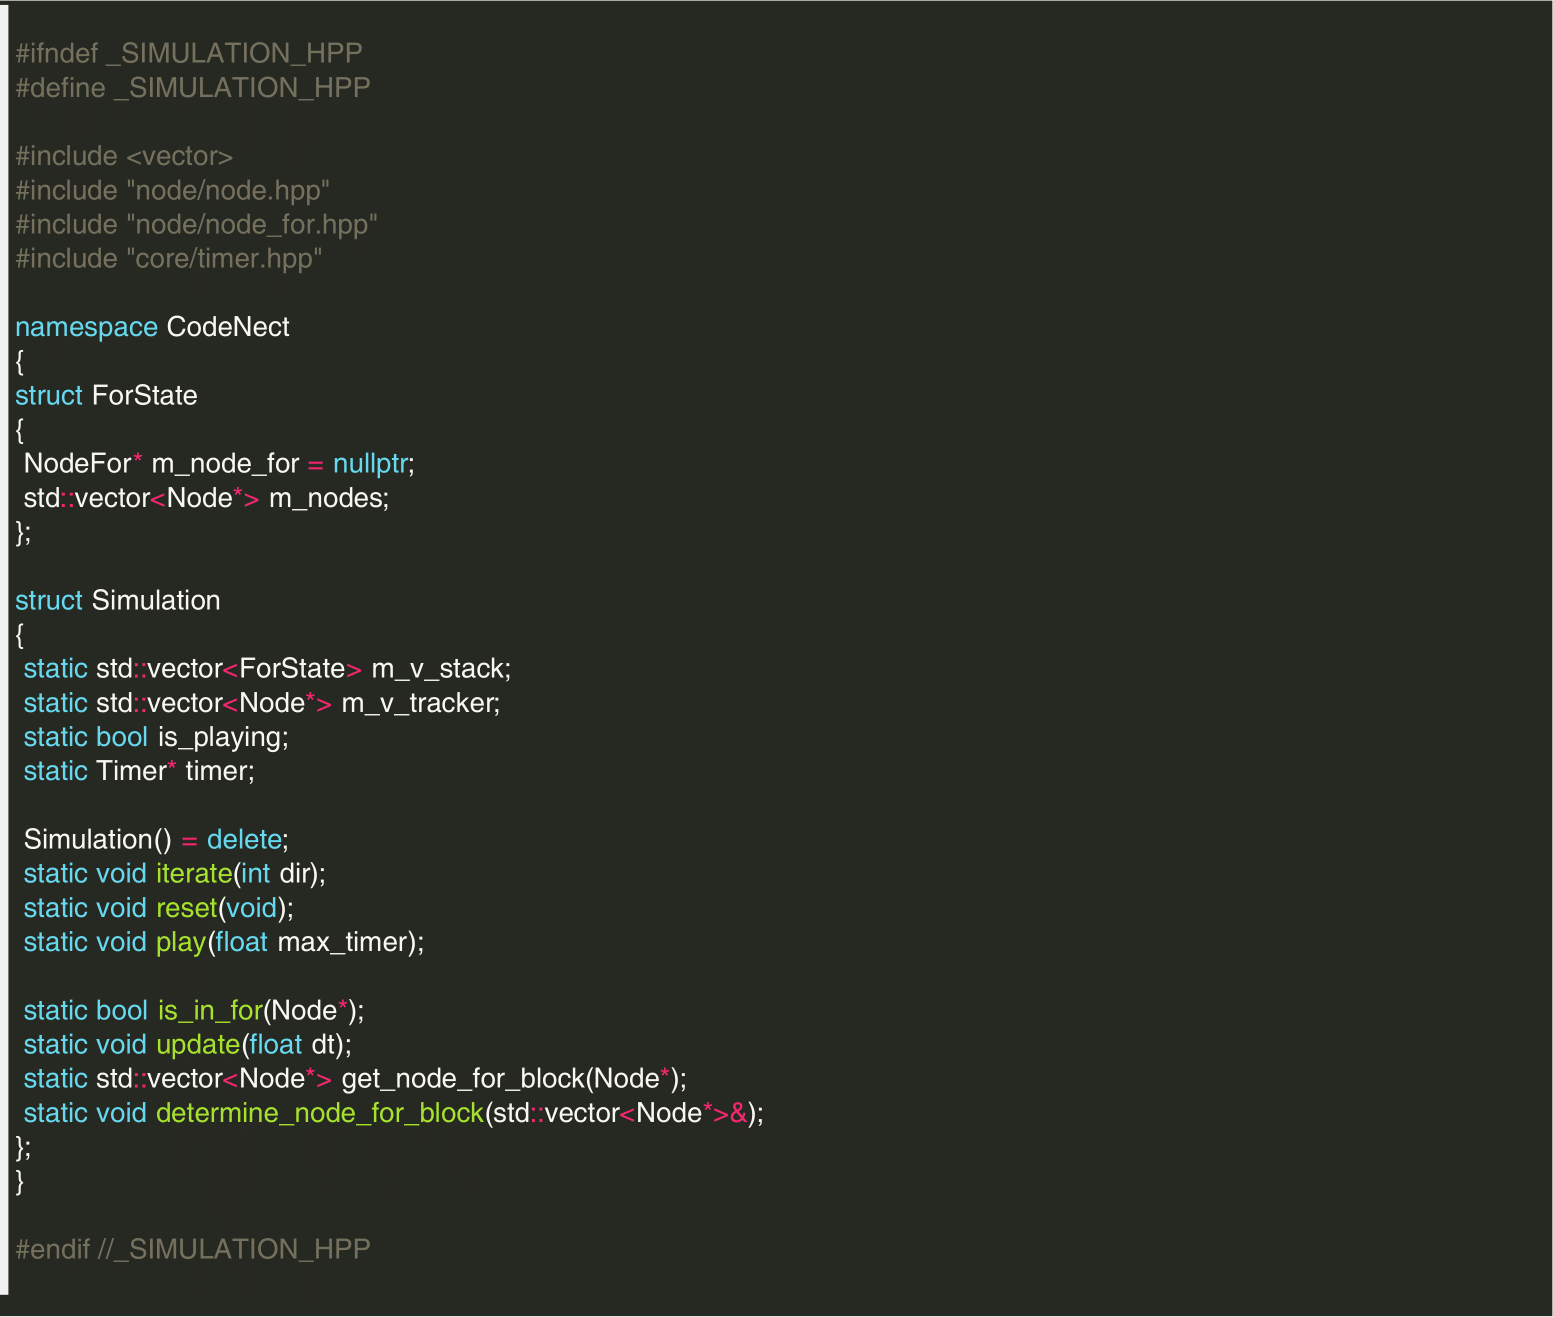
\includegraphics[width=\textwidth]{figures/code/simulation.png}
\end{figure}
\begin{figure}[H]
	 \centering
	 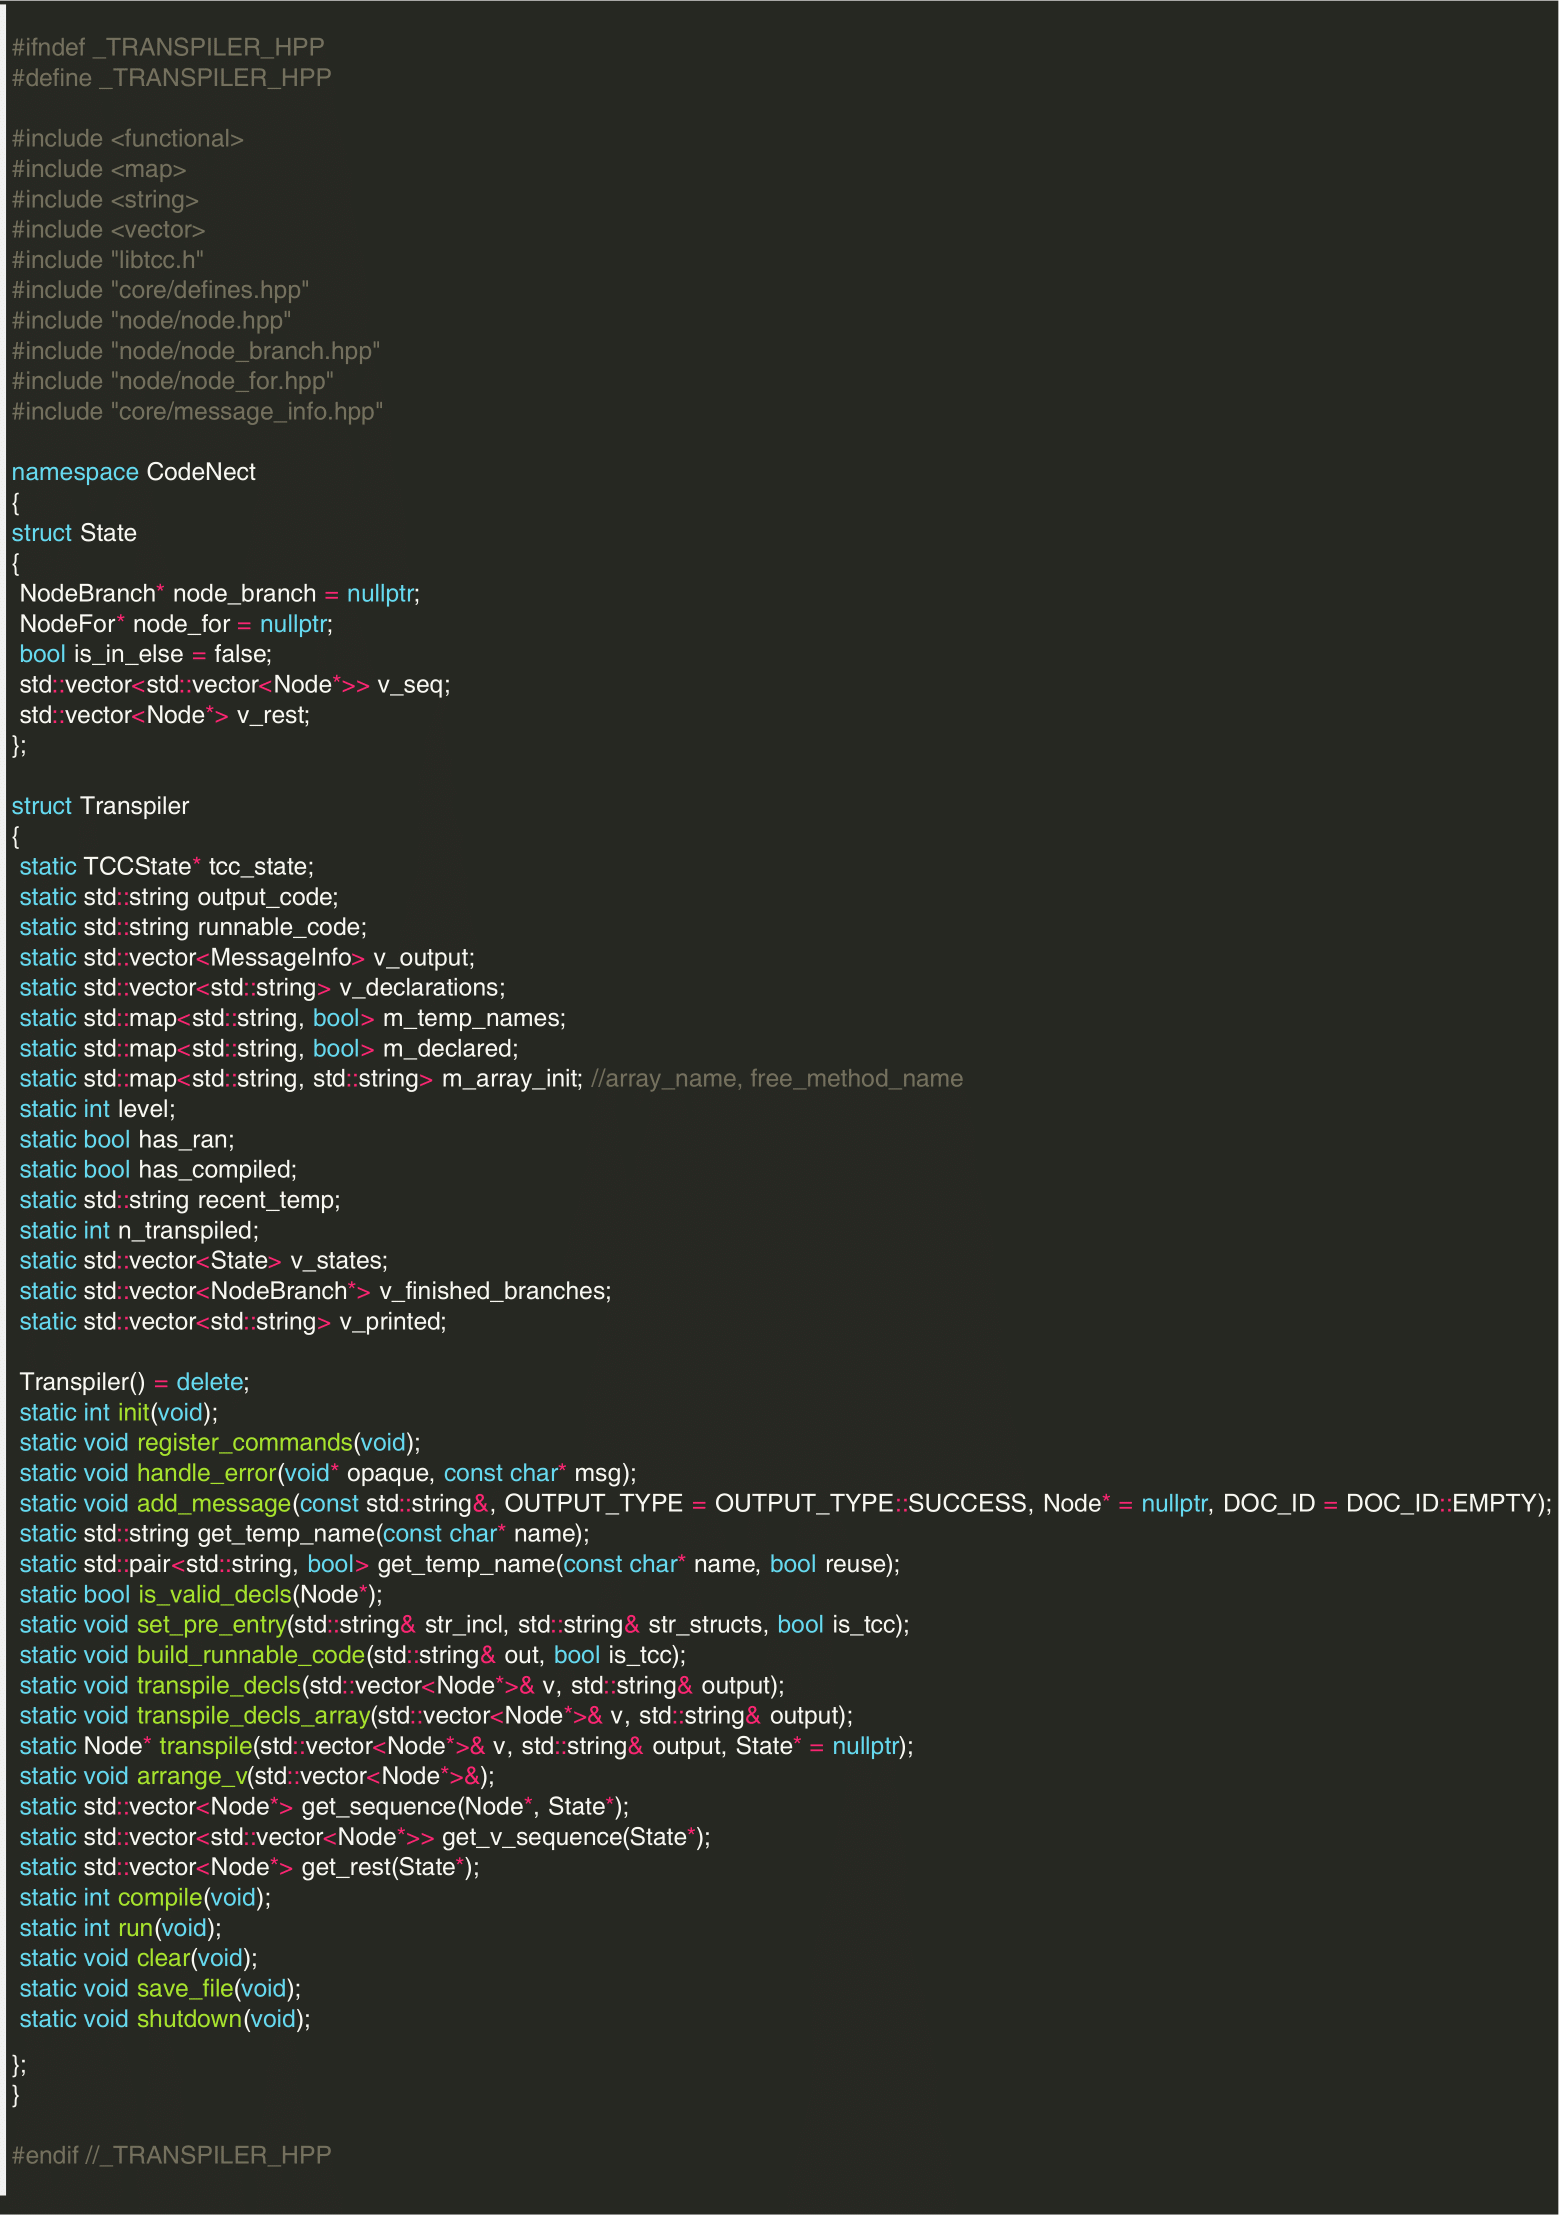
\includegraphics[width=\textwidth]{figures/code/transpiler.png}
\end{figure}

		% \clearpage
\app{Other Appendices}
\null\vfill
\begin{figure}[H]
	 \centering
	 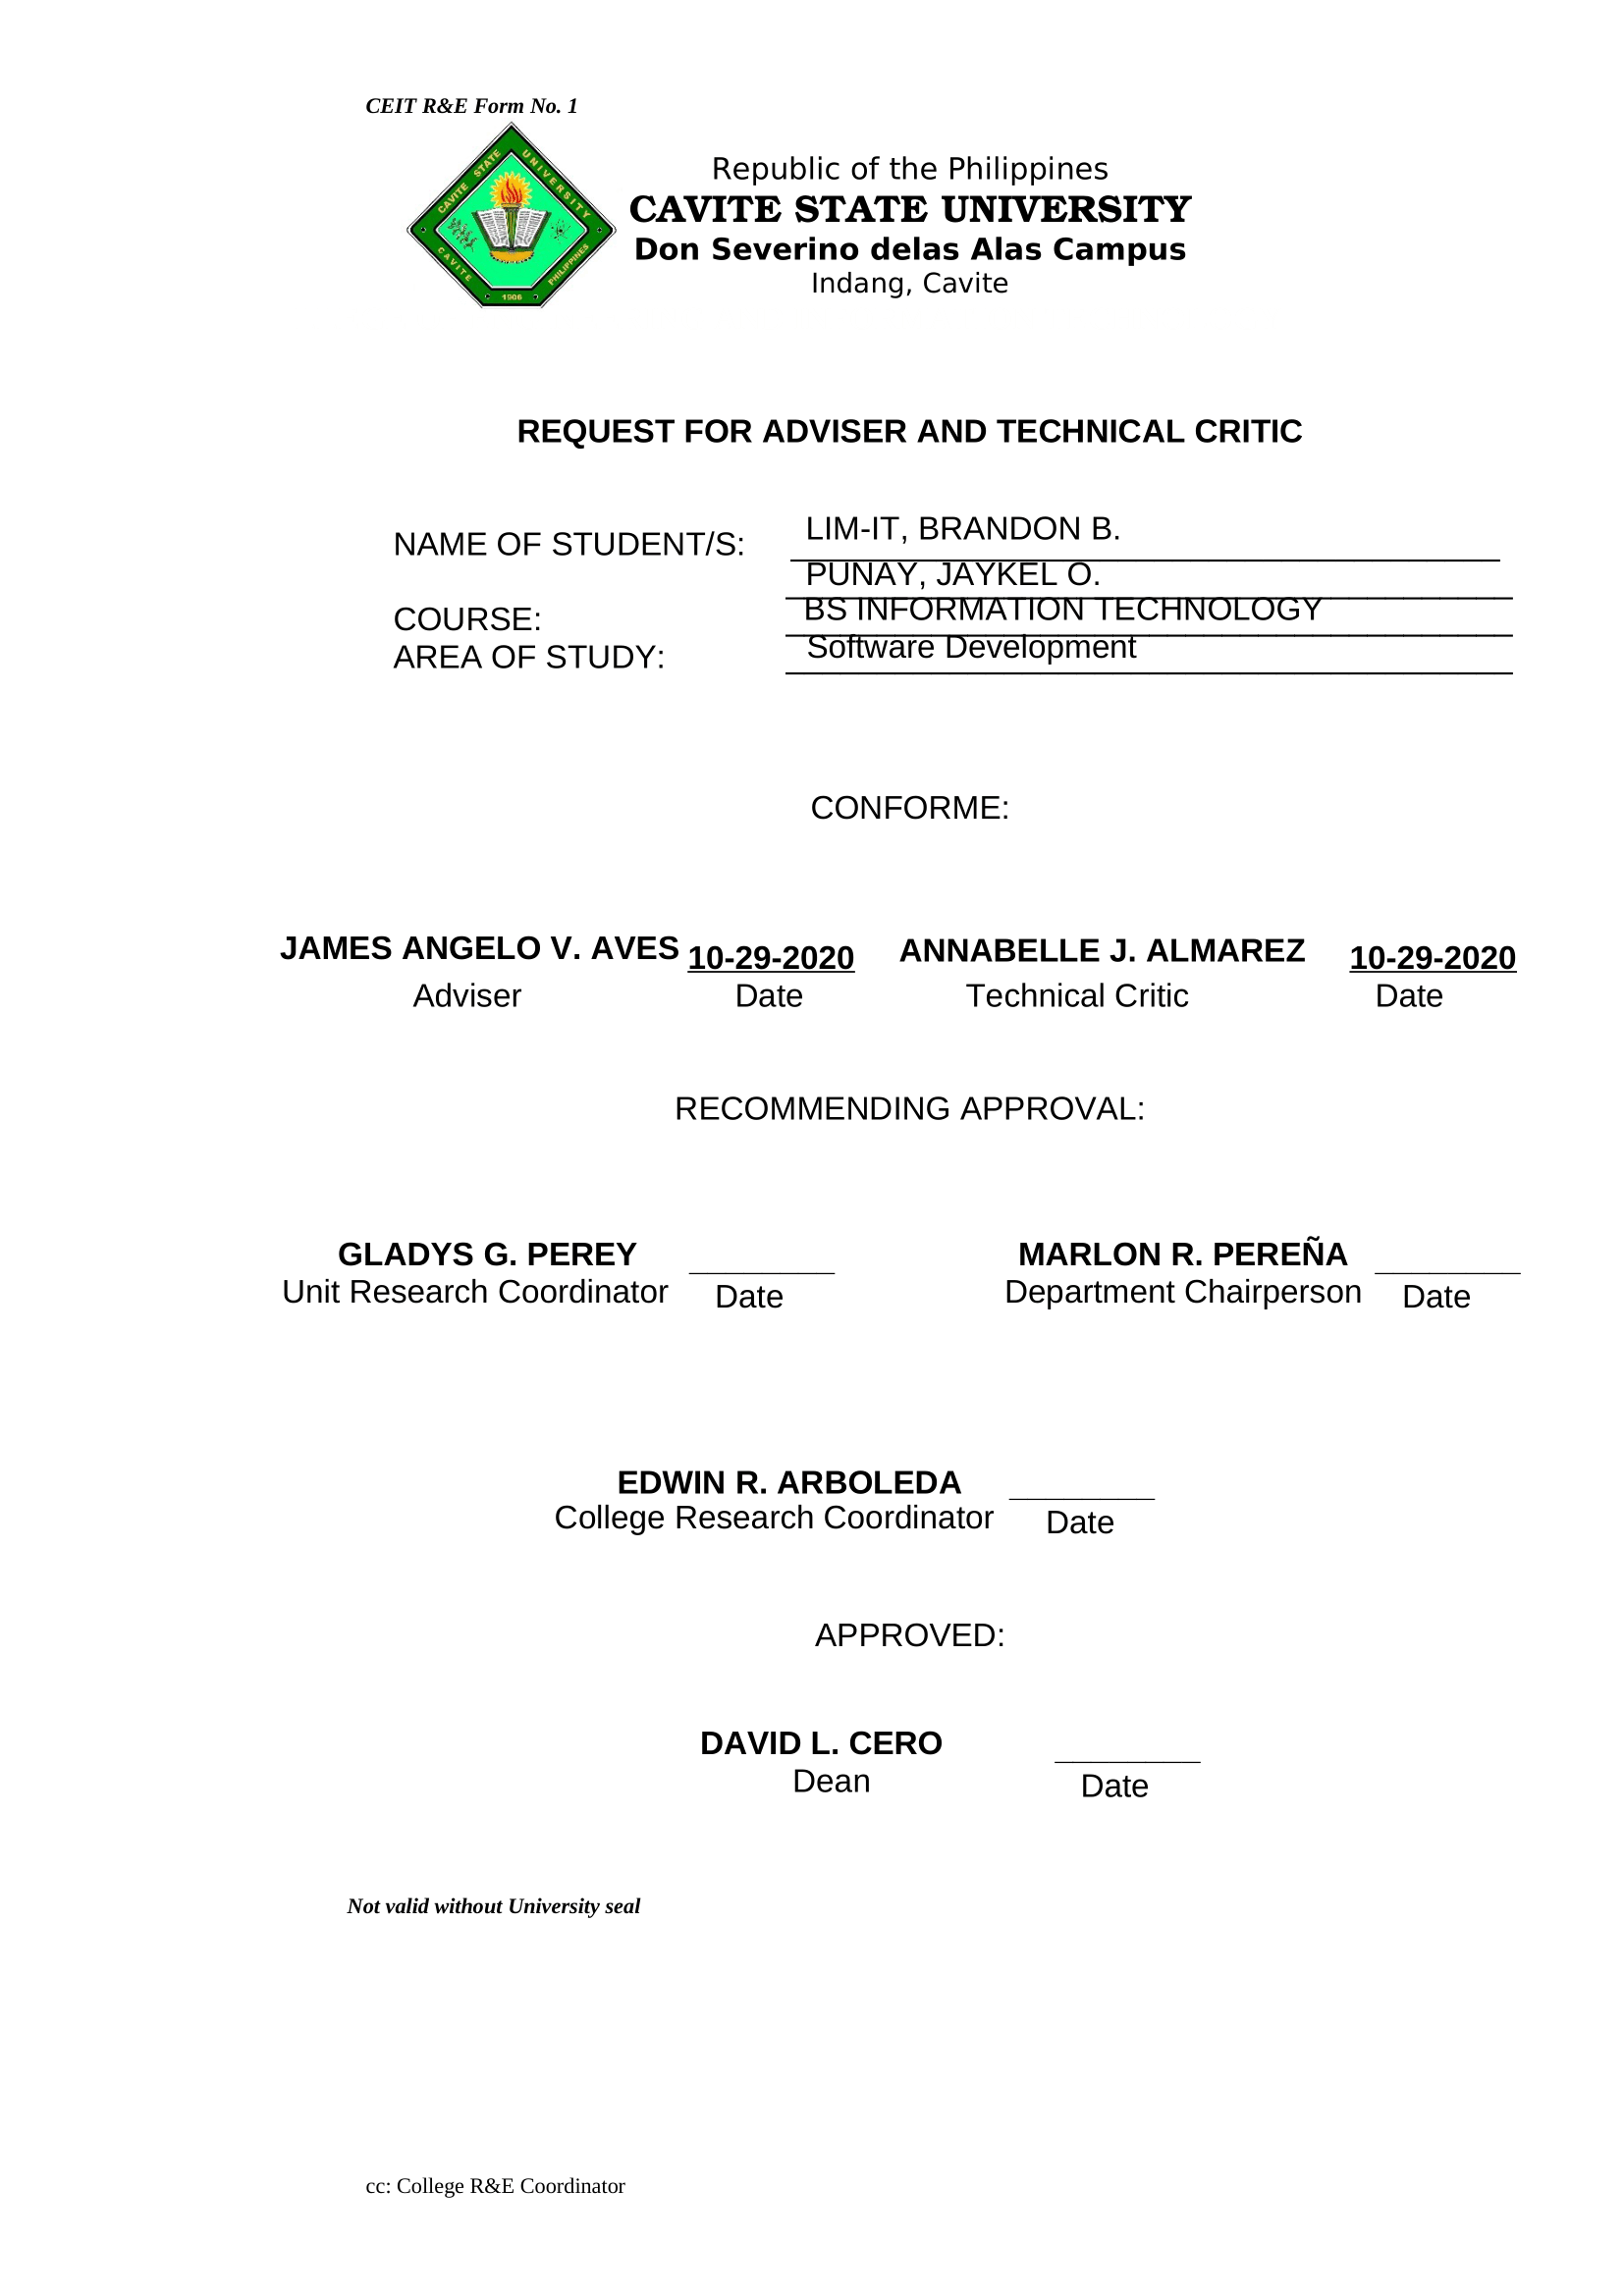
\includegraphics[width=\textwidth]{figures/1_adviser_tc_approval.png}
	 \caption[]{Adviser and Technical Critic Approval Form}
	 \label{fig:adviser_tc_approval}
\end{figure}
\clearpage
\null\vfill
\begin{figure}[H]
	 \centering
	 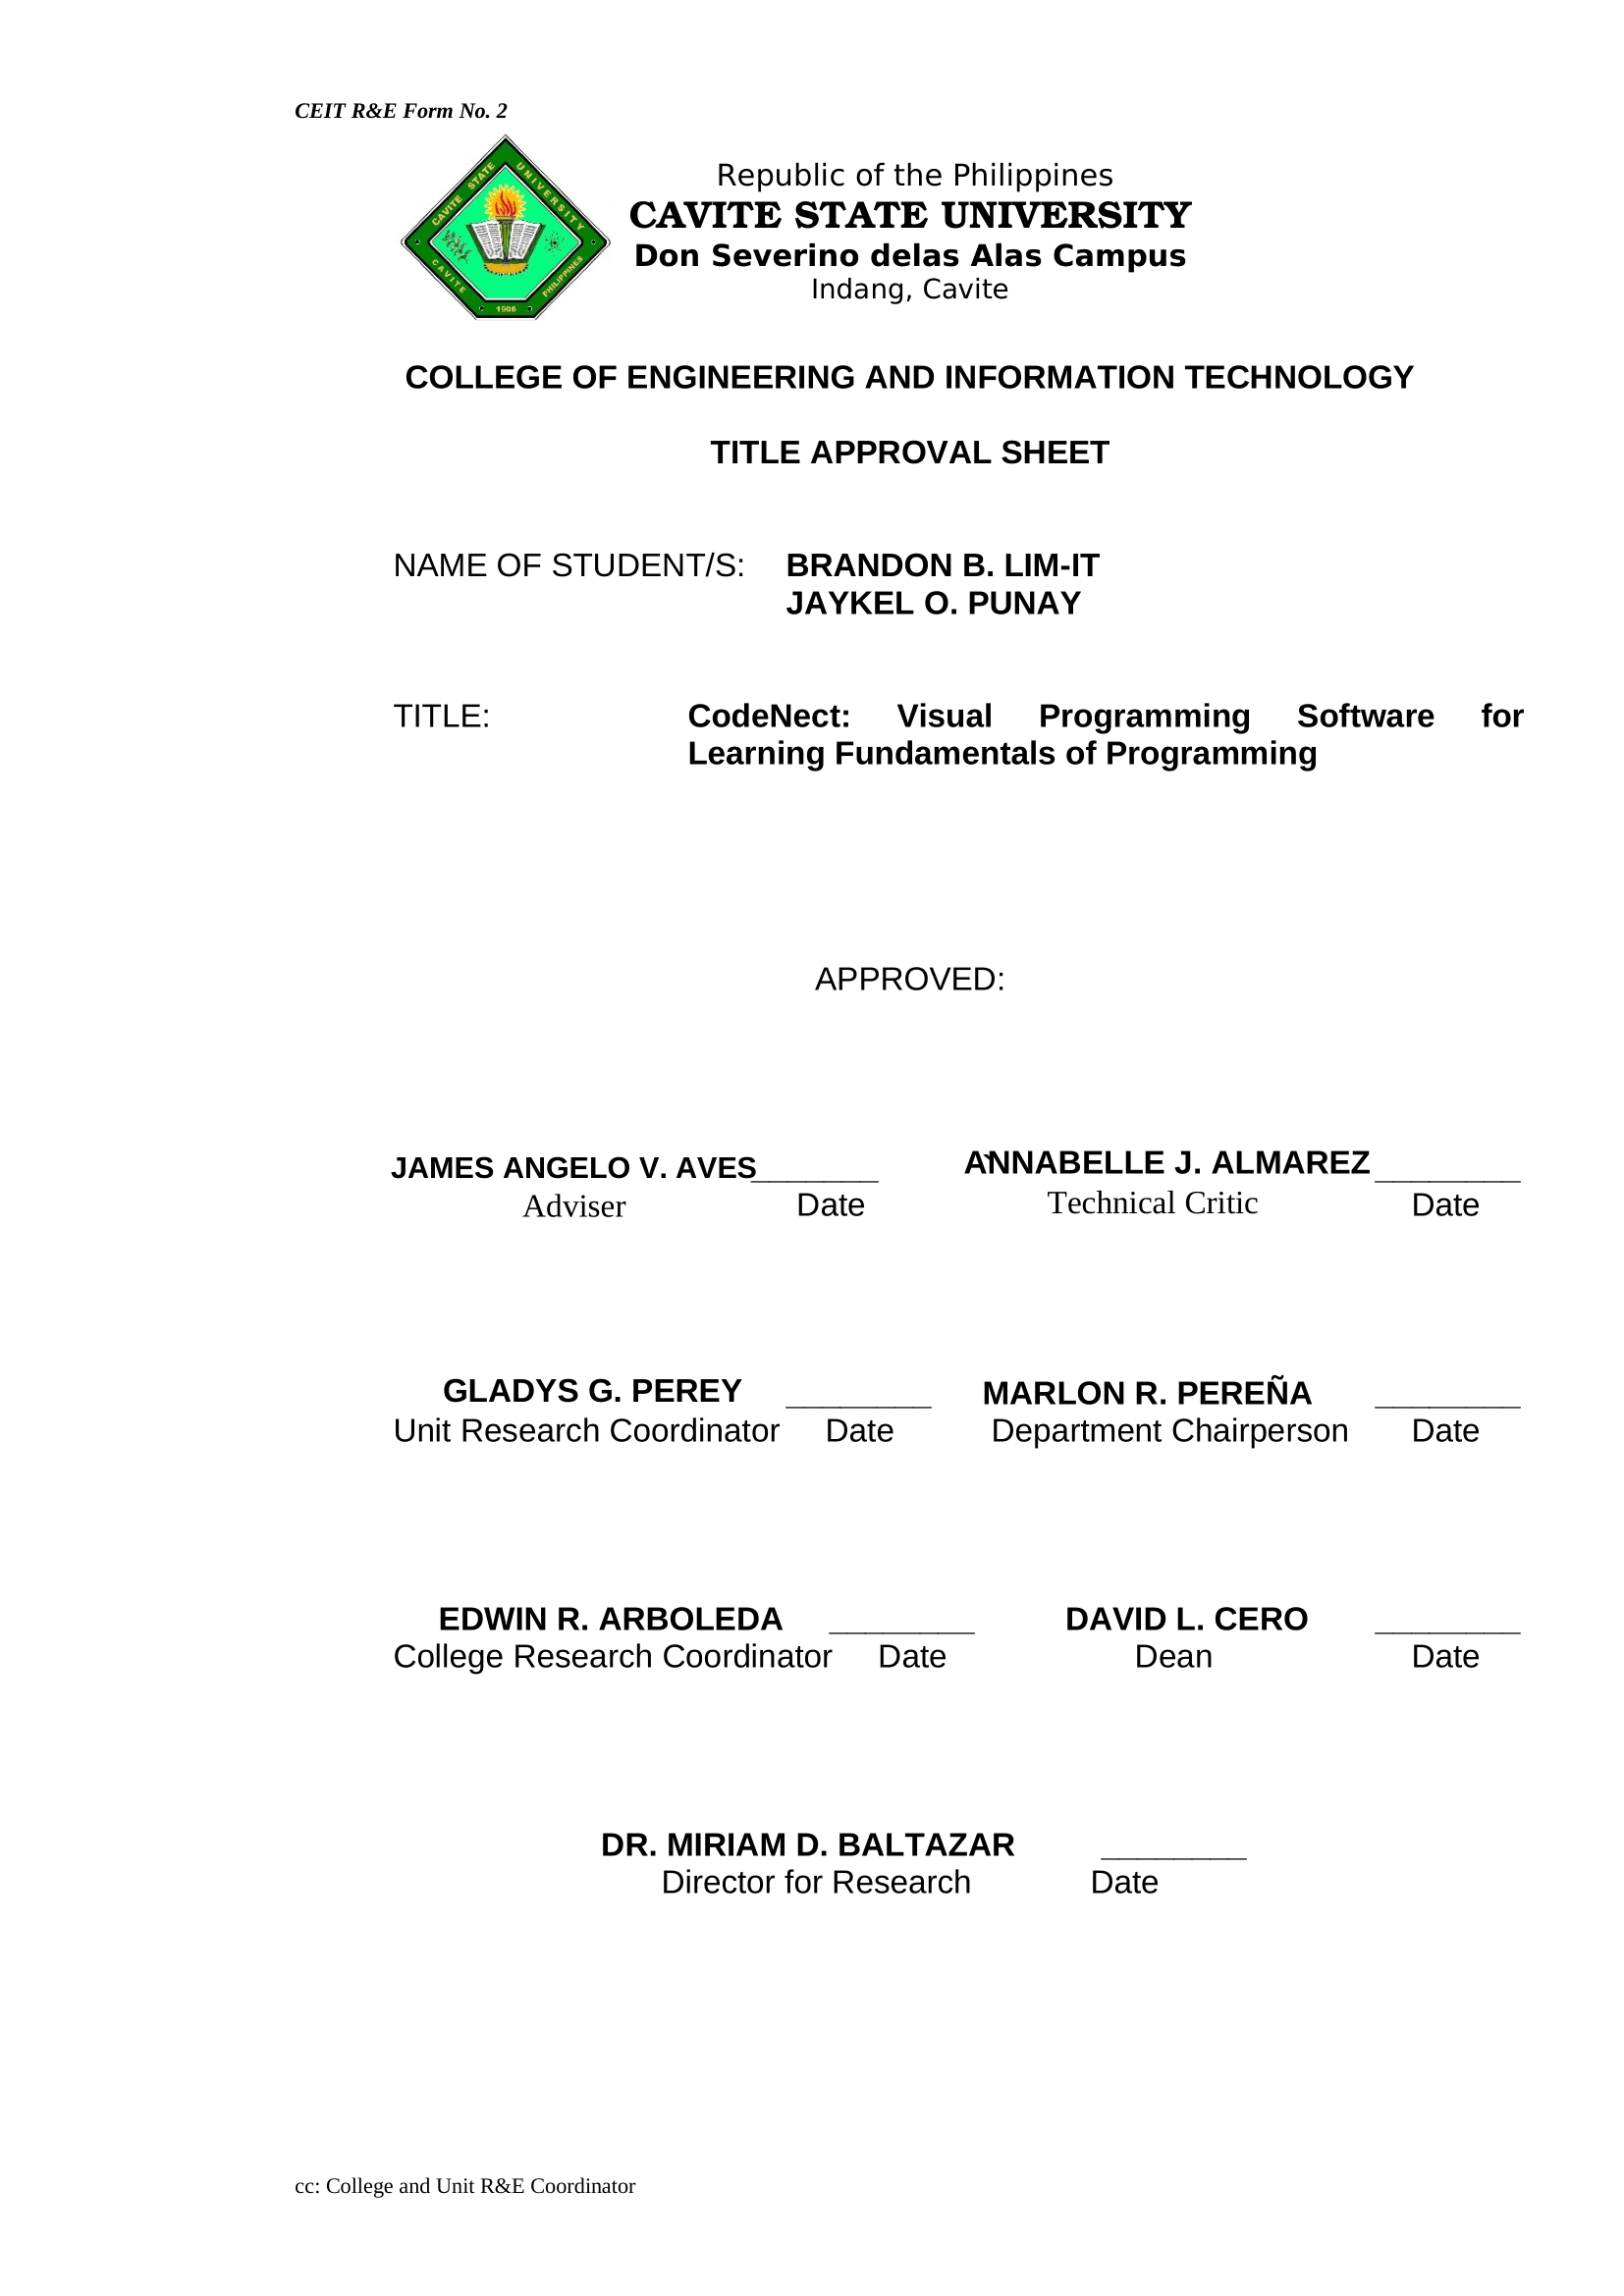
\includegraphics[width=\textwidth]{figures/2_title_approval.png}
	 \caption[]{Title Approval Form}
	 \label{fig:title_approval}
\end{figure}
\clearpage
\null\vfill
\begin{figure}[H]
	 \centering
	 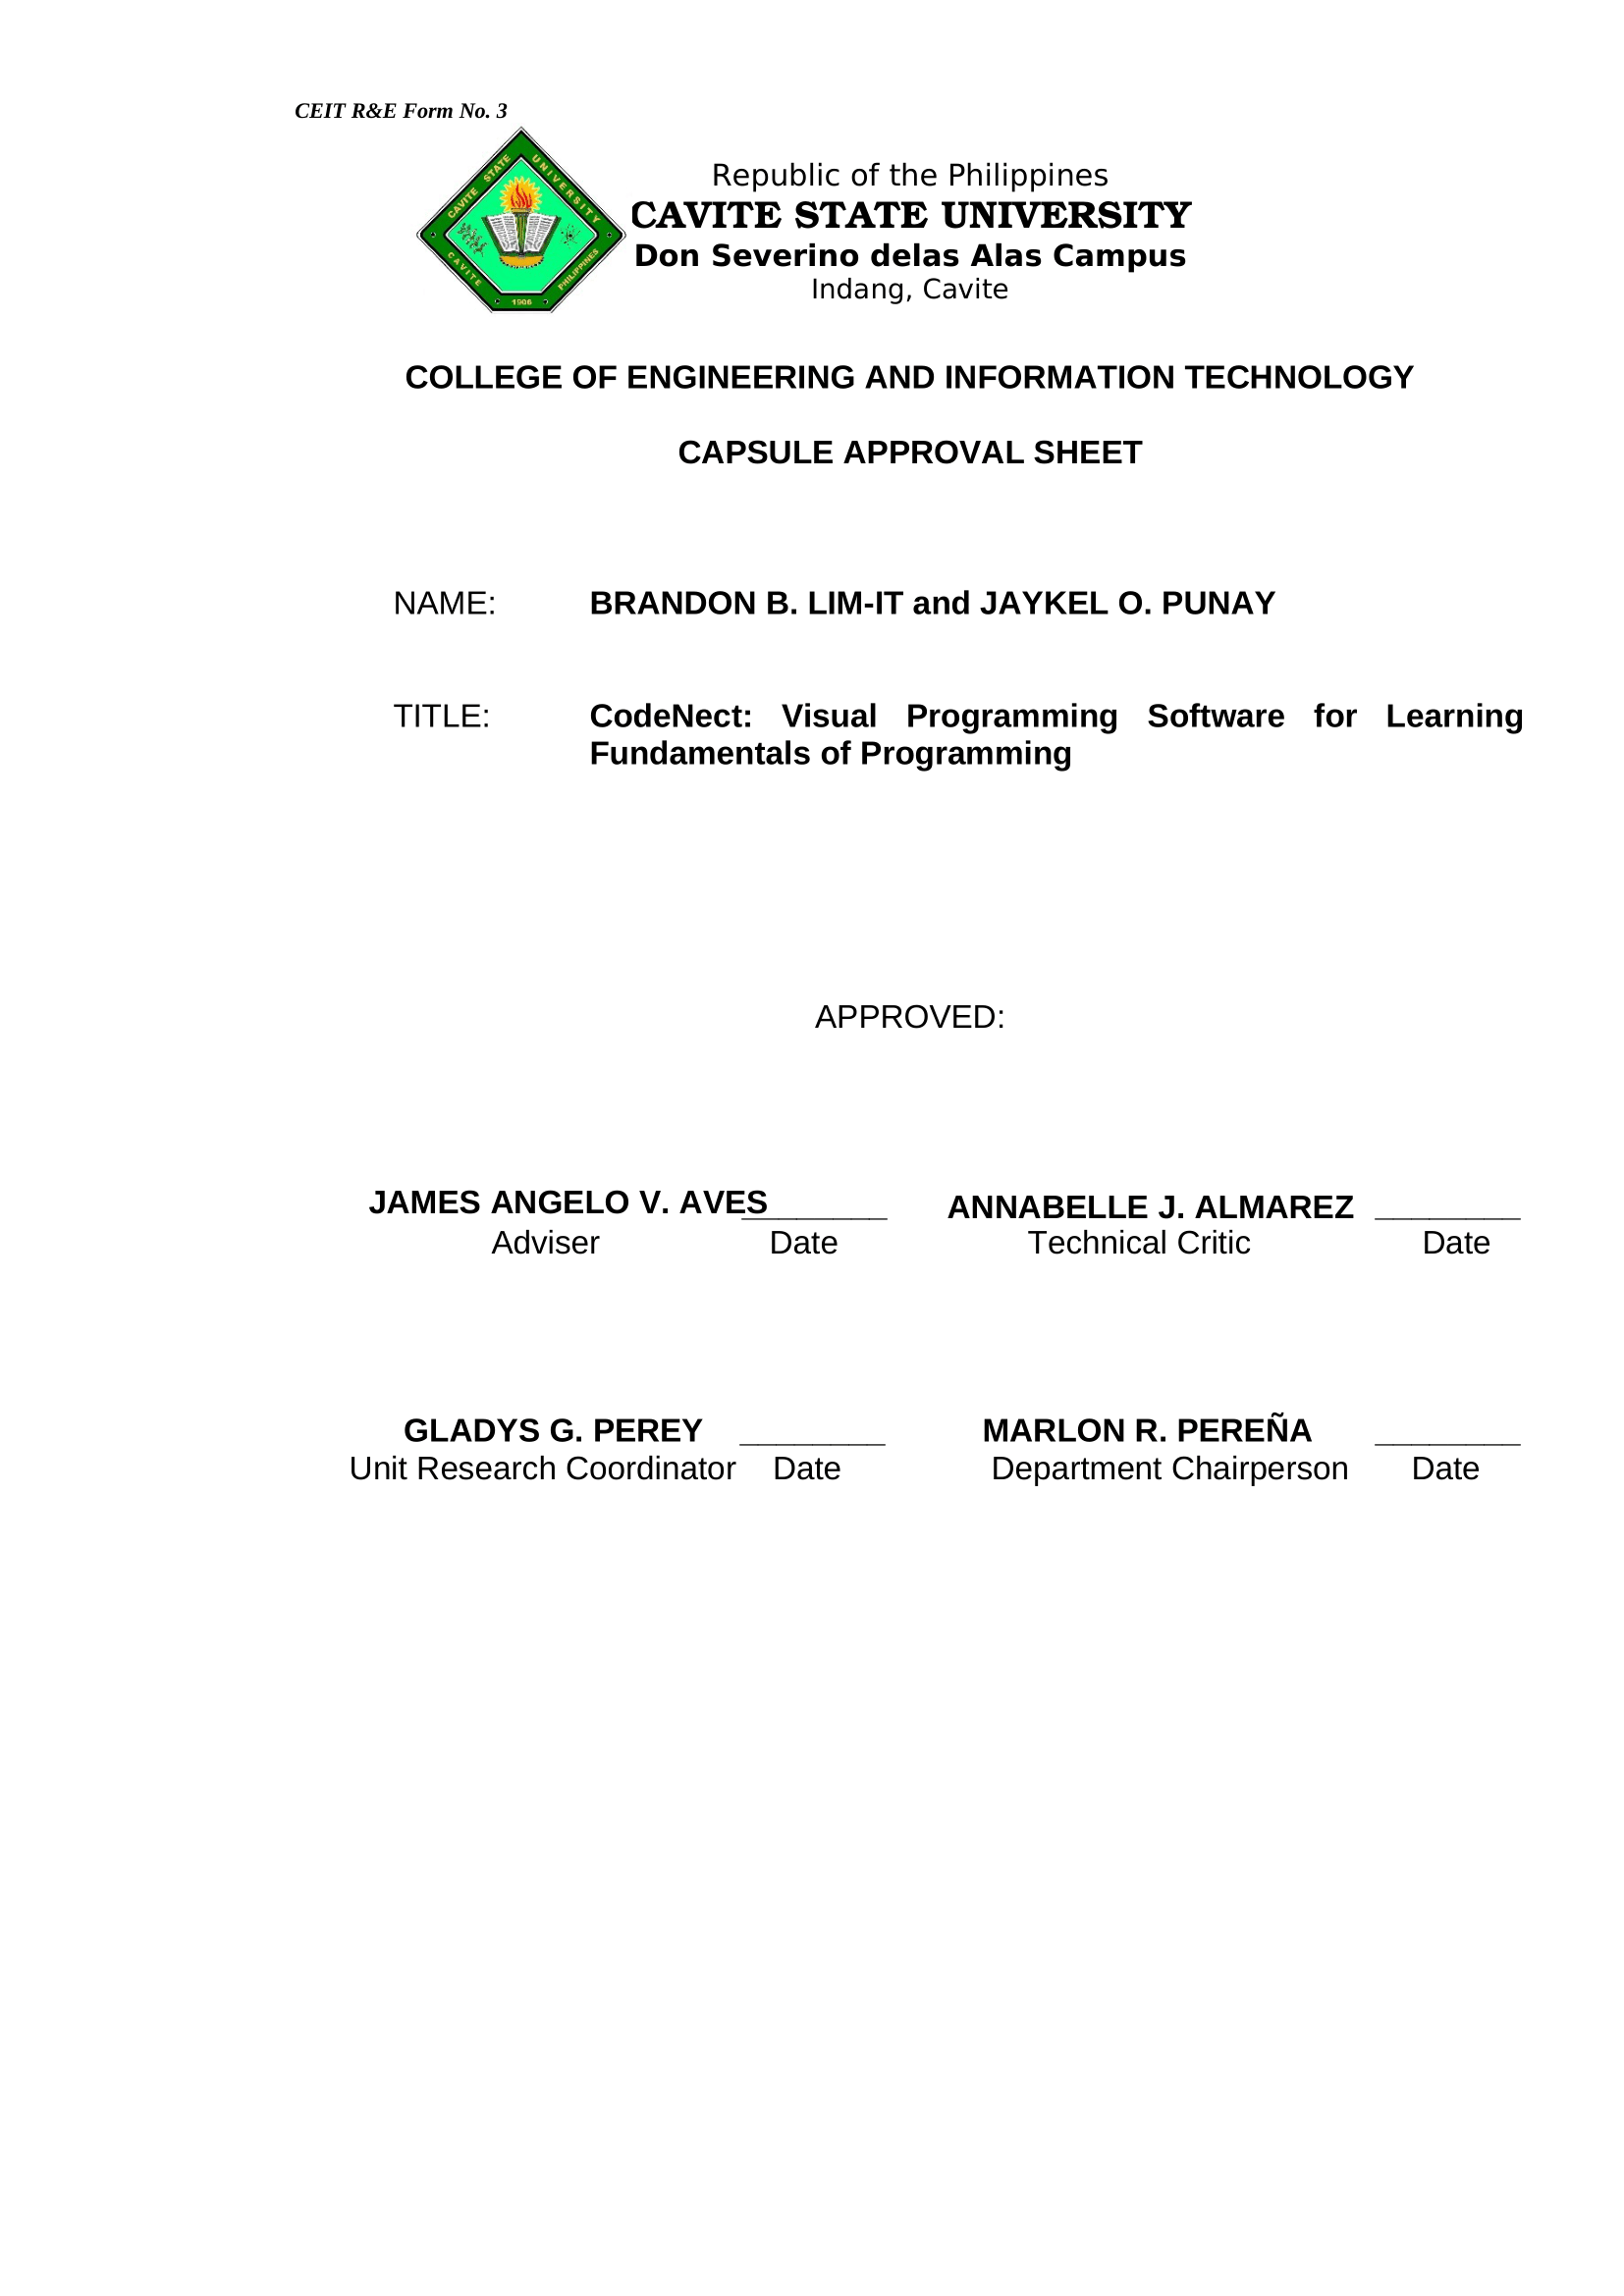
\includegraphics[width=\textwidth]{figures/3_capsule_approval.png}
	 \caption[]{Capsule Approval Form}
	 \label{fig:capsule_approval}
\end{figure}
\clearpage
\null\vfill
\begin{figure}[H]
	 \centering
	 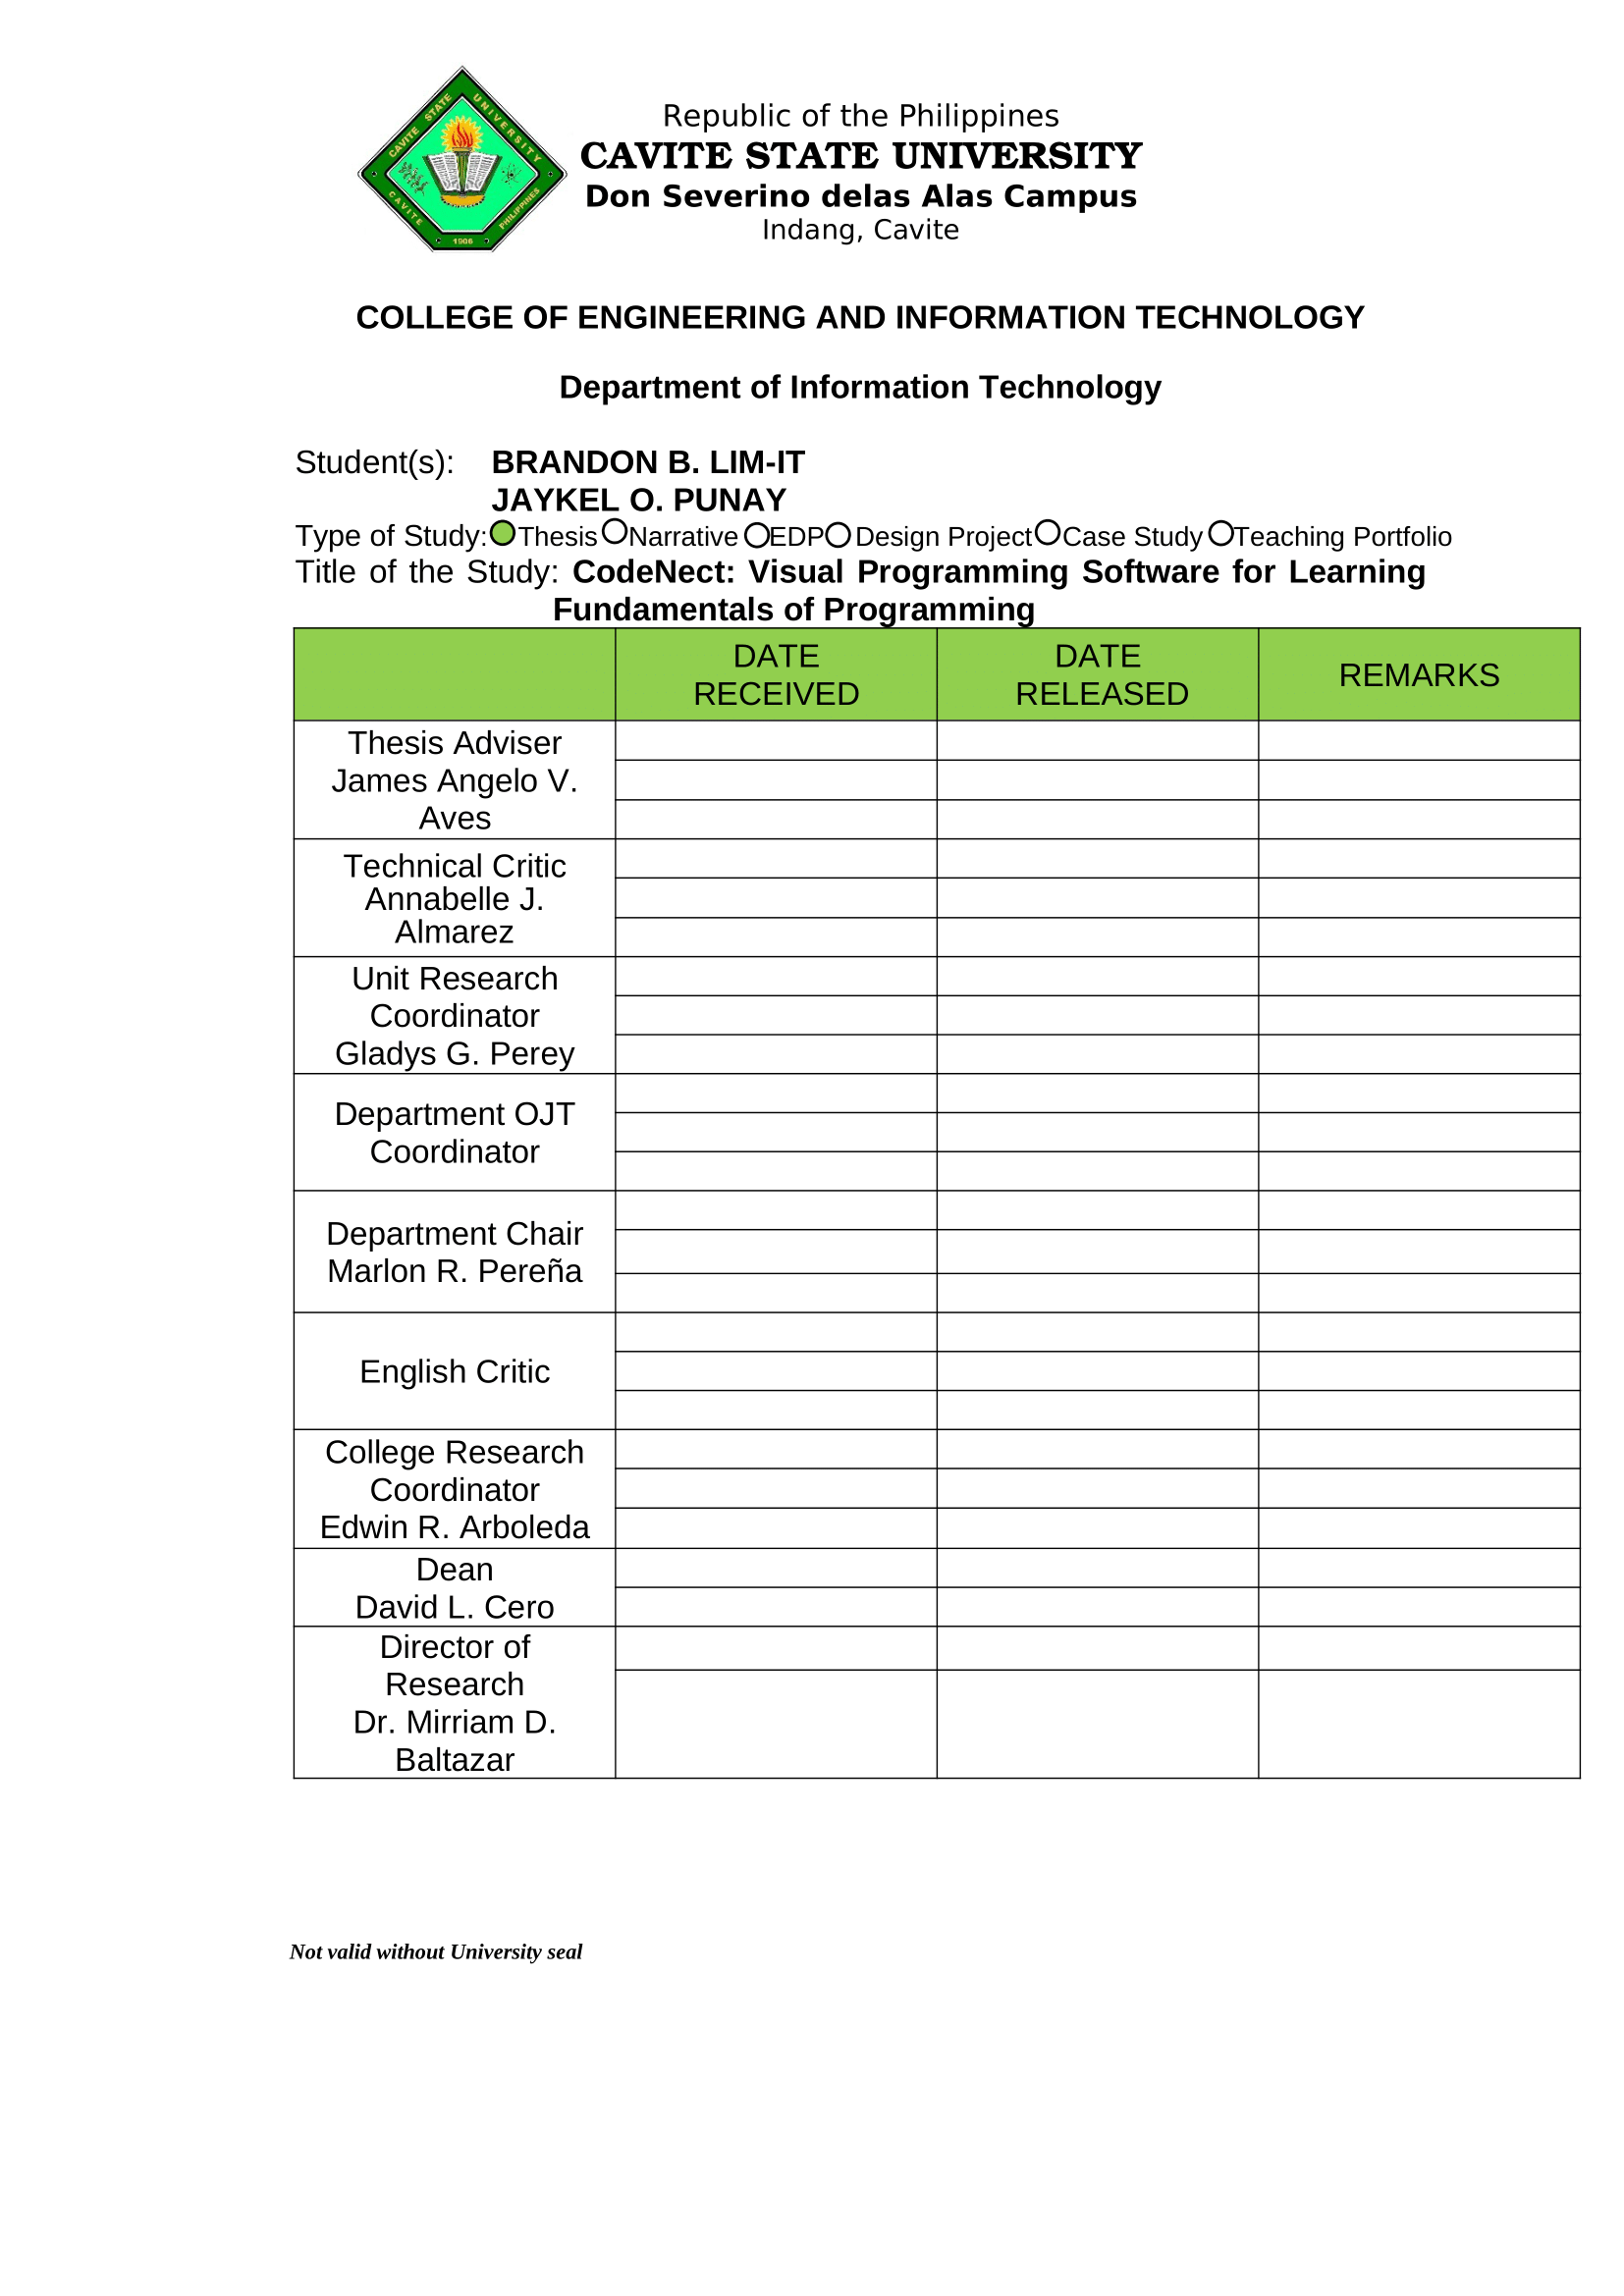
\includegraphics[width=\textwidth]{figures/4_routing_slip.png}
	 \caption[]{Routing Slip Form}
	 \label{fig:routing_slip}
\end{figure}
\clearpage
\null\vfill
\begin{figure}[H]
	 \centering
	 
\includegraphics[width=\textwidth]{figures/5_request_defense.png}
	 \caption[]{Request for Defense Form}
	 \label{fig:request_defense}
\end{figure}


	\end{center}
\end{doublespace}
